\documentclass[11pt,a4paper]{article}

\usepackage[utf8]{inputenc}
\usepackage[T1]{fontenc}
\usepackage{lmodern}
\usepackage[english]{babel}
\usepackage[margin=2.5cm]{geometry}
\usepackage{amsmath,amssymb}
\usepackage{graphicx}
\usepackage{caption}
\usepackage{subcaption}
\usepackage{float}
\usepackage{array}
\usepackage{tabularx}
\usepackage{xcolor}
\usepackage{indentfirst}
\usepackage{titlesec}
\usepackage{url}
% Optional (uncomment on Overleaf or if pdfescape is installed in MiKTeX):
% \usepackage[colorlinks=true,linkcolor=blue!55!black,citecolor=blue!55!black,urlcolor=blue!55!black]{hyperref}

\captionsetup{font=small,labelfont=bf}
\graphicspath{{figures/}}

% Helper macros for clean academic table rules
\newcommand{\toprule}{\noalign{\hrule height 0.9pt}\noalign{\vskip 2pt}}
\newcommand{\midrule}{\noalign{\vskip 2pt}\noalign{\hrule height 0.45pt}\noalign{\vskip 2pt}}
\newcommand{\bottomrule}{\noalign{\vskip 2pt}\noalign{\hrule height 0.9pt}}
\renewcommand{\arraystretch}{1.18}

% Section heading spacing
\titleformat{\section}{\large\bfseries}{\thesection.}{0.6em}{}
\titleformat{\subsection}{\normalsize\bfseries}{\thesubsection}{0.6em}{}
\titleformat{\subsubsection}{\normalsize\itshape\bfseries}{\thesubsubsection}{0.6em}{}

\title{\textbf{4D Behavioral Modeling, Hardware Security, and Visual Prototyping of Polymorphic Circuits Based on BP SB-FET Transistors in an Open-Source Environment}}

% TODO: Fill in authors, affiliations, and emails in the final version
\author{
  Author 1\thanks{Department / Institution --- E-mail: \texttt{author1@institution.edu}} \and
  Author 2\thanks{Department / Institution --- E-mail: \texttt{author2@institution.edu}}
}

\date{\today}

\begin{document}

\maketitle

\begin{abstract}
\noindent\textit{[Abstract reserved for final drafting after completing the Introduction and Theoretical Background sections. This work documents the 4D behavioral translation of the ambipolar 2D black phosphorus Schottky-barrier FET (BP SB-FET) to \texttt{ngspice-47}, its cross-validation against HSPICE, ultra-low-voltage inverter characterization, polymorphic logic primitives, polarity-locked 6T SRAM retention collapse, cryptographic full adder design, non-standard voltage operating boundaries, DPA asymmetry-versus-cost trade-offs across seven polymorphic tuples, and the interactive web platform BP-FET Studio.]}
\end{abstract}

\vspace{0.5em}
\noindent\textbf{Keywords:} 2D Transistors; Black Phosphorus; Polymorphic Logic; Hardware Security; Differential Power Analysis; 6T SRAM; \texttt{ngspice-47}.

\section{Introduction}\label{sec:introduction}

\noindent\textit{[Section reserved for later drafting.]}

% TODO: Insert contextualization on hardware security in conventional CMOS
% technologies versus reconfigurable 2D devices, the tool gap regarding
% proprietary simulators (HSPICE/Verilog-A and MATLAB), general and specific
% objectives of this work, and paper organization.

\section{Theoretical Background}\label{sec:theoretical_background}

\noindent\textit{[Section reserved for later drafting.]}

% TODO: Insert theoretical background on:
% 1. Physics of two-dimensional black phosphorus FETs (BP SB-FET),
%    Schottky barriers, WKB tunneling, and ambipolar suppression via polarity gate.
% 2. Five-terminal architecture (d, g, s, g1, g2) and polymorphic logic gates.
% 3. Hardware security foundations: logic locking, IC camouflaging,
%    Differential Power Analysis (DPA), and SRAM memory locking (SNM and Read-Assist).

\section{Methodology}\label{sec:methodology}

\subsection{Open-Source Computational Flow and Experimental Suite Organization}\label{sec:met_flow}

All experimental and numerical developments in this work were structured within a fully open-source and reproducible computational environment, eliminating the original dependency on proprietary commercial tools---namely Synopsys HSPICE with Verilog-A (\texttt{\$table\_model}) support and MATLAB---used in the reference files of Wu et al.~\cite{wu2020reconfigurable}. The adopted circuit simulation engine is \texttt{ngspice-47} (executed in batch mode via \texttt{ngspice\_con.exe}), coupled with Python routines (\texttt{numpy}, \texttt{pandas}, and \texttt{matplotlib}) responsible for parameterized SPICE netlist generation, automated metric extraction, statistical analyses, and figure plotting.

To ensure traceability and continuous verification, the experiments were organized into eight self-contained modules (\texttt{00} through \texttt{07}) under \texttt{experimentos/}, executed sequentially by the master orchestrator \texttt{run\_all.py}, which re-simulates every netlist and validates the integrity of all 66 generated artifacts (libraries, netlists, CSV tables, and figures). Complementarily, an interactive web-based visual prototyping platform (\textit{BP-FET Studio}, in \texttt{simulador\_web/}) was built and directly coupled to \texttt{ngspice-47}. Table~\ref{tab:module_summary} summarizes the methodological scope of each component in the suite.

\begin{table}[htbp]
\centering
\caption{Structure of the experimental suite in \texttt{ngspice-47} + Python and the interactive visual platform.}
\label{tab:module_summary}
\scriptsize
\begin{tabularx}{\textwidth}{>{\raggedright\arraybackslash}p{1.05cm} >{\raggedright\arraybackslash}p{2.35cm} >{\raggedright\arraybackslash}X >{\raggedright\arraybackslash}p{3.45cm}}
\toprule
\textbf{Module} & \textbf{Domain / Analysis} & \textbf{Methodological Scope} & \textbf{Main Deliverables} \\
\midrule
\texttt{00} & Device (DC) & 4D translation of experimental tables to native SPICE and cross-validation against HSPICE \texttt{.printtr0}. & \texttt{bp\_\allowbreak ari\_\allowbreak ngspice.lib}, 5 netlists, 2 CSVs, 4 figs. \\
\texttt{01} & 2T Inverter (DC/Tran) & $V_{DD}$ sweeps from $1.0\ \text{V}$ down to $0.2\ \text{V}$ with and without $V_{fb}$ compensation; transient switching ($0.5\ \text{fF}$). & 2 netlists, 1 CSV, 2 figs. \\
\texttt{02} & 4T Gates (Tran) & Dynamic runtime transmutation at $t=20\ \text{ns}$ for \texttt{NAND}$\leftrightarrow$\texttt{NOR} ($0.8\ \text{V}$) and \texttt{XOR}$\leftrightarrow$\texttt{XNOR} ($1.5\ \text{V}$). & 2 netlists, 1 CSV, 2 figs. \\
\texttt{03} & DPA \& Noise (DC/Stat.) & Python port of DPA datasets, 3D Monte Carlo ($N=250$), and floating retention; $5\times 5$ supply sweep in \texttt{ngspice}. & 1 netlist, 3 CSVs, 4 figs. \\
\texttt{04} & 6T SRAM (Tran/DC) & Mechanism B implementation ($30\ \text{ns}$), butterfly curves, SNM, and \textit{Wordline Read-Assist} ($0.30\ \text{V}$). & 2 netlists, 1 CSV, 2 figs. \\
\texttt{05} & 28T Full Adder (Tran) & Multi-stage polymorphic adder with 2-bit key $(K_1, K_0)$, level shifting, and Hamming Distance. & 1 netlist, 1 CSV, 2 figs. \\
\texttt{06} & Boundaries (Staircase) & 292-point sweep under non-standard voltages within the measured LUT domain. & 3 netlists, 2 CSVs, 3 figs. \\
\texttt{07} & DPA Pareto \& FA (Tran) & Evaluation of 7 polymorphic tuples, Monte Carlo ($N=250$), and 3-profile Full Adder benchmark. & 4 netlists, 3 CSVs, 4 figs. \\
\texttt{Web} & Interactive Platform & High/low-level graph-to-SPICE compiler, transistor X-Ray viewer, DPA oscilloscope, and E2E tests. & HTTP server, compiler, E2E suite \\
\bottomrule
\end{tabularx}
\end{table}

\subsection{4D Behavioral Model Translation of the BP SB-FET to \texttt{ngspice-47}}\label{sec:met_model}

In the original Verilog-A model (\texttt{bp\_ari.va}), the ambipolar black phosphorus Schottky-barrier field-effect transistor (BP SB-FET) is represented by a five-terminal \texttt{ari} block (\texttt{d, g, s, g1, g2}) parameterized by a relative width multiplier $W$, querying two four-dimensional experimental lookup tables (\texttt{BP\_ARI\_\allowbreak dataN.txt}, 1,810 rows, and \texttt{BP\_ARI\_\allowbreak dataP.txt}, 759 rows) via the \texttt{\$table\_model} directive~\cite{wu2020reconfigurable}. Because \texttt{ngspice-47} does not natively execute 4D \texttt{\$table\_model} tables, Module~\texttt{00} (\texttt{gerar\_\allowbreak modelo\_\allowbreak e\_\allowbreak validar.py}) constructs a native behavioral subcircuit \texttt{.subckt ARI d g s g1 g2 W=1.0} (\texttt{bp\_ari\_\allowbreak ngspice.lib}) in its refined \texttt{v2} (4D Surface) formulation.

To support bidirectional circuits in which drain and source swap roles depending on the input vector or polarity key---such as pass-transistor \texttt{XOR}/\texttt{XNOR} gates, SRAM access transistors, and locked-mode source followers---the subcircuit defines effective bilateral source references:
\begin{equation}\label{eq:bilateral_ref}
V_{g,n} = V_g - \min(V_d, V_s), \quad V_{g1,n} = V_{g1} - \min(V_d, V_s),
\end{equation}
\begin{equation}\label{eq:bilateral_ref_p}
V_{g,p} = V_g - \max(V_d, V_s), \quad V_{g1,p} = V_{g1} - \max(V_d, V_s).
\end{equation}
These expressions preserve the exact nominal biases whenever $V_{ds} \ge 0$ in the \textit{n-FET} branch and $V_{ds} \le 0$ in the \textit{p-FET} branch while maintaining current continuity upon $V_{ds}$ reversal.

Over this reference frame, the full two-dimensional transfer surface $(V_{g1}, V_{g2})$ at $|V_{ds}| = 0.8\ \text{V}$ is reconstructed via bilinear interpolation using piecewise-linear (\texttt{pwl}) hat functions with flat external clamping at $\pm 1000\ \text{V}$ to prevent unphysical extrapolation and ensure MNA solver convergence:
\begin{itemize}
    \item \textbf{\textit{n-FET} branch:} $7 \times 4 = 28$ experimental slices spanning $V_{g1} \in [-0.1,\ 1.1]\ \text{V}$ (in $0.2\ \text{V}$ steps) and $V_{g2} \in \{0.2,\allowbreak\ 0.4,\allowbreak\ 0.8,\allowbreak\ 1.0\}\ \text{V}$, swept across $V_{g,n} \in [-0.8,\ 1.1]\ \text{V}$.
    \item \textbf{\textit{p-FET} branch:} $8 \times 4 = 32$ experimental slices spanning $V_{g1} \in [-1.5,\ -0.1]\ \text{V}$ (in $0.2\ \text{V}$ steps) and $V_{g2} \in \{-1.5,\allowbreak\ -1.2,\allowbreak\ -1.1,\allowbreak\ -0.9\}\ \text{V}$, swept across $V_{g,p} \in [-1.5,\ 0.0]\ \text{V}$. Explicitly incorporating the measured $V_{g2} = -1.5\ \text{V}$ plane captures the actual flat-band voltage shift ($\Delta V_{fb} \approx -0.25\ \text{V}$) present in the experimental dataset, which was not captured by the preliminary 1D scalar scaling (\texttt{v1}).
\end{itemize}

To capture the triode and saturation regions as a joint function of the main gate and drain-source voltage, \texttt{v2} replaces the global analytical factor $\tanh(2.5\,V_{ds})/\tanh(2.0)$ of \texttt{v1} with gate-specific 2D experimental factors $f_{ds,n}(V_{g,n}, V_{ds})$ (6 slices over $V_{g,n} \in [0.1,\ 1.1]\ \text{V}$) and $f_{ds,p}(V_{g,p}, V_{ds})$ (5 slices over $V_{g,p} \in [-1.5,\ -0.7]\ \text{V}$), extracted from the experimental output sweeps, normalized at $|V_{ds}| = 0.8\ \text{V}$, and extended as strictly monotonic odd \texttt{pwl} functions with finite ohmic conductance at $V_{ds} = 0\ \text{V}$. The drain-source current is imposed by the behavioral current source:
\begin{equation}\label{eq:bp_current}
I_{ds} = W \cdot \begin{cases}
I_n(V_{g1,n},\, V_{g2,s},\, V_{g,n}) \cdot f_{ds,n}(V_{g,n},\, V_{ds}), & \text{if } V(g2,s) > 0\ \text{V}, \\
I_p(V_{g1,p},\, V_{g2,s},\, V_{g,p}) \cdot f_{ds,p}(V_{g,p},\, V_{ds}), & \text{if } V(g2,s) \le 0\ \text{V},
\end{cases}
\end{equation}
shunted by an auxiliary resistor $R_{\mathrm{gmin}} = 10^{12}\ \Omega$ for numerical stability. It is worth noting that, identically to the original \texttt{bp\_ari.va} file, \texttt{bp\_ari\_ngspice.lib} is purely quasi-static and omits intrinsic gate and overlap capacitances ($C_{gs}, C_{gd}, C_{g2s}$); accordingly, all transient simulations reported below include explicit load and nodal capacitances ($0.05\ \text{fF}$ to $1.0\ \text{fF}$).

Model validation was performed via five DC testbenches (\texttt{sim\_\allowbreak N\_\allowbreak transfer.sp}, \texttt{sim\_\allowbreak P\_\allowbreak transfer.sp}, \texttt{sim\_\allowbreak N\_\allowbreak output.sp}, \texttt{sim\_\allowbreak P\_\allowbreak output.sp}, and \texttt{sim\_\allowbreak polarity\_\allowbreak gate.sp}), directly comparing \texttt{v1} and \texttt{v2} against the official Synopsys HSPICE \texttt{.printtr0} reference outputs via root-mean-square error (RMSE), mean absolute error (MAE), maximum error, and coefficient of determination ($R^2$). Device metrics $I_{\mathrm{on}}$, $I_{\mathrm{off}}$, $I_{\mathrm{on}}/I_{\mathrm{off}}$ ratio, and minimum subthreshold swing ($SS_{\min}$) were also extracted at $|V_{ds}| = 0.8\ \text{V}$.

\subsection{Ultra-Low-Voltage Inverter and Polymorphic Gate Characterization}\label{sec:met_inv_poly}

In Module~\texttt{01}, the complementary BP SB-FET inverter ($W_{\mathrm{PU}} = W_{\mathrm{PD}} = 1.0$) was biased at nominal conduction operating points (\textit{n-FET} pull-down at $V_{g1,n} = 1.1\ \text{V},\ V_{g2,n} = 0.8\ \text{V}$ and \textit{p-FET} pull-up at $V_{g1,p} = V_{DD} - 1.5\ \text{V},\ V_{g2,p} = V_{DD} - 1.2\ \text{V}$). DC voltage transfer characteristic (VTC) sweeps were executed in \texttt{inv\_vtc.sp} ($0 \to V_{DD}$ in $2\ \text{mV}$ steps) for $V_{DD} \in \{1.0,\ 0.8,\ 0.6,\ 0.4,\ 0.2\}\ \text{V}$ under two configurations:
\begin{enumerate}
    \item \textbf{Direct coupling:} input voltage $V_{\mathrm{in}}$ applied directly to the gate terminals without offset (\texttt{off}$_n = \text{off}_p = 0$).
    \item \textbf{Electrostatic $V_{fb}$ compensation:} controlled gate offsets $\text{off}_n = -0.02 - 0.5\,V_{DD}$ and $\text{off}_p = 0.5\,V_{DD} - 0.58$, aligning both branches at their peak subthreshold gain point ($V_{gs,n,\mathrm{eff}} = -0.02\ \text{V}$ and $V_{gs,p,\mathrm{eff}} = -0.58\ \text{V}$) when $V_{\mathrm{in}} = V_{DD}/2$.
\end{enumerate}
From the VTC curves, percentage output swing $(V_{\mathrm{out}}(0)-V_{\mathrm{out}}(V_{DD}))/V_{DD}$, switching threshold $V_M$, peak differential gain $|A_v|_{\max} = \max|dV_{\mathrm{out}}/dV_{\mathrm{in}}|$, and static noise margins $NM_L$ and $NM_H$ (at unity-slope points $dV_{\mathrm{out}}/dV_{\mathrm{in}} = -1$) were extracted. Additionally, \texttt{inv\_tran.sp} evaluated transient switching ($14\ \text{ns}$) with $C_{\mathrm{load}} = 0.5\ \text{fF}$ at $V_{DD} = 1.0\ \text{V}$ and $0.6\ \text{V}$.

In Module~\texttt{02}, transient simulations ($40\ \text{ns}$, $20\ \text{ps}$ time step, $C_{\mathrm{out}} = 0.3\ \text{fF}$) were performed on the two 4-transistor polymorphic primitives introduced in~\cite{wu2020reconfigurable}, sweeping all input vectors $(A,B) \in \{00, 01, 10, 11\}$ in $5\ \text{ns}$ windows with runtime key switching at $t = 20\ \text{ns}$:
\begin{itemize}
    \item \textbf{\texttt{NAND} $\leftrightarrow$ \texttt{NOR} (\texttt{poly\_nand\_nor.sp}, $V_{DD} = 0.8\ \text{V}$):} parallel top network ($W=1.0$) tied to \texttt{rtop}/\texttt{gtop} and series bottom network ($W=2.0$, intermediate node capacitance $C_{n1}=0.1\ \text{fF}$) tied to \texttt{rbot}/\texttt{gbot}. Under $\text{Key}=0$ (\texttt{NAND}), biases are set to $(r_{\mathrm{top}}, g_{\mathrm{top}}, r_{\mathrm{bot}}, g_{\mathrm{bot}}) = (0.8,\ -0.4,\ 0.0,\ 0.8)\ \text{V}$; under $\text{Key}=1$ (\texttt{NOR}), supply rails and polarities permute to $(0.0,\ 0.8,\ 0.8,\ -0.7)\ \text{V}$.
    \item \textbf{\texttt{XOR} $\leftrightarrow$ \texttt{XNOR} (\texttt{poly\_xor\_xnor.sp}, $V_{DD} = 1.5\ \text{V}$, $V_{\mathrm{in}} = 1.1\ \text{V}$):} four identical transistors ($W=1.0$) in a symmetric bridge driven by differential inputs $(A,\overline{A})$ on terminals \texttt{g} and $(B,\overline{B})$ on auxiliary terminals \texttt{g1}, alternating $(r_{\mathrm{top}}, g_{\mathrm{top}}, r_{\mathrm{bot}}, g_{\mathrm{bot}})$ between $(1.5,\ 0.0,\ 0.0,\ 0.8)\ \text{V}$ ($\text{Key}=0$, \texttt{XOR}) and $(0.0,\ 0.8,\ 1.5,\ 0.0)\ \text{V}$ ($\text{Key}=1$, \texttt{XNOR}).
\end{itemize}

\subsection{DPA Security, Statistical Robustness, and Voltage Boundaries}\label{sec:met_dpa_boundary}

In Module~\texttt{03}, the proprietary MATLAB scripts of~\cite{wu2020reconfigurable} were fully ported to Python (\texttt{analisar\_\allowbreak dpa\_\allowbreak e\_\allowbreak robustez.py}) to process transient supply current waveforms $|I(V_{DD})|$ of the \texttt{NAND}/\texttt{NOR} and \texttt{XOR}/\texttt{XNOR} families ($0\text{--}30\ \mu\text{s}$ window), 250-sample Monte Carlo datasets of simultaneous $V_{DD}$ and $V_{SS}$ rail noise per gate (classifying logic levels around a $0.40\ \text{V}$ threshold), and floating-node retention traces (\texttt{bblc1}) up to $111\ \mu\text{s}$ following $100\ \text{ns}$, $250\ \text{ns}$, and $500\ \text{ns}$ pulses. As an independent parametric verification of the translated model, \texttt{sim\_\allowbreak supply\_\allowbreak noise.sp} executed a $5 \times 5$ grid in \texttt{ngspice-47} sweeping $V_{DD} \in [0.65,\ 0.95]\ \text{V}$ and $V_{SS} \in [-0.10,\ +0.10]\ \text{V}$ on the 4T \texttt{NAND} gate to measure the static differential margin $V_{\mathrm{out}}(00) - V_{\mathrm{out}}(11)$.

In Module~\texttt{06}, circuit behavior under non-standard operating voltages was investigated via staircase PWL sweeps using four parallel cells representing \texttt{00}, \texttt{01}, \texttt{10}, and \texttt{11}. Methodologically, all terminal biases were strictly constrained within the experimentally measured LUT domain: $V(g2,s)_n \in [+0.20,\ +1.00]\ \text{V}$ and $V(g2,s)_p \in [-1.50,\ -0.90]\ \text{V}$, deliberately avoiding the unmeasured gap $(-0.90,\ +0.20)\ \text{V}$. In total, 292 operating points were simulated across three experiments:
\begin{enumerate}
    \item \textbf{\texttt{NAND}/\texttt{NOR} ($V_{DD} \times$ Polarity, 70 points):} 7 supply levels $V_{DD} \in \{0.25,\allowbreak\ 0.35,\allowbreak\ 0.50,\allowbreak\ 0.65,\allowbreak\ 0.80,\allowbreak\ 0.95,\allowbreak\ 1.10\}\ \text{V}$ crossed with 5 polarity pairs inside the LUT ($\text{Sub-pol Min}\ +0.2/-0.9\ \text{V}$, $\text{Sub-pol Mod}\ +0.4/-1.1\ \text{V}$, $\text{Nom.\ NAND}\ +0.8/-1.2\ \text{V}$, $\text{Nom.\ NOR}\ +0.8/-1.5\ \text{V}$, and $\text{Over-pol}\ +1.0/-1.5\ \text{V}$) for $\text{Key} \in \{0, 1\}$.
    \item \textbf{\texttt{NAND}/\texttt{NOR} ($V(g2,s)_n \times V(g2,s)_p$ Asymmetry, 72 points):} $6 \times 6$ grid at $V_{DD} = 0.80\ \text{V}$ sweeping $V(g2,s)_n \in \{0.20,\allowbreak\ 0.30,\allowbreak\ 0.40,\allowbreak\ 0.60,\allowbreak\ 0.80,\allowbreak\ 1.00\}\ \text{V}$ and $V(g2,s)_p \in \{-0.90,\allowbreak\ -1.00,\allowbreak\ -1.10,\allowbreak\ -1.20,\allowbreak\ -1.35,\allowbreak\ -1.50\}\ \text{V}$ for $\text{Key} \in \{0, 1\}$.
    \item \textbf{\texttt{XOR}/\texttt{XNOR} ($V_{DD} \times V_{\mathrm{in}}$ and fixed gate, 150 points):} 5 supply levels $V_{DD} \in \{0.60,\allowbreak\ 0.80,\allowbreak\ 1.00,\allowbreak\ 1.20,\allowbreak\ 1.50\}\ \text{V}$ $\times$ 5 input amplitudes $V_{\mathrm{in}} \in \{0.40,\allowbreak\ 0.60,\allowbreak\ 0.80,\allowbreak\ 1.10,\allowbreak\ 1.30\}\ \text{V}$ under nominal ($+0.8/-1.5\ \text{V}$) and sub-polarized ($+0.2/-0.9\ \text{V}$) bias for both keys (100 points), plus 50 points evaluating fixed $V_{g,\mathrm{top}} = 0\ \text{V}$ over $V_{DD} \in [0.90,\ 1.50]\ \text{V}$.
\end{enumerate}
Each normalized output $V_{\mathrm{out}}/V_{DD}$ was discretized into \texttt{'1'} ($\ge 0.75$), \texttt{'0'} ($\le 0.25$), or \texttt{'X'} ($0.25 < V_{\mathrm{out}}/V_{DD} < 0.75$), categorizing each operating point as \texttt{CORRETA} (target Boolean function), \texttt{OUTRA\_\allowbreak FUNCAO} (valid digital levels realizing a different Boolean function), or \texttt{INDEFINIDO\_\allowbreak ANALOGICO} (at least one output settling in the analog transition region \texttt{'X'}).

\subsection{6T SRAM Cell with Polarity-Controlled Retention Locking (Mechanism B)}\label{sec:met_sram}

In Module~\texttt{04}, a 6T SRAM cell implementing polarity-inversion retention locking (\textit{Mechanism B}) was modeled and simulated in \texttt{ngspice-47} (\texttt{ARI\_sram\_mecB\_ngspice.sp}). Unlike polymorphic logic gates that permute supply rails, Mechanism B keeps the power rails strictly fixed at $V_{DD} = 1.0\ \text{V}$ and $V_{SS} = 0.0\ \text{V}$, using the security key exclusively to dynamically invert the conduction polarity of the transistors inside the cross-coupled inverters.

The six \texttt{ARI} transistors adopt width ratios sized to balance read stability and writeability: pull-up devices \texttt{XPU1}, \texttt{XPU2} with $W = 1.0$; pull-down devices \texttt{XPD1}, \texttt{XPD2} with $W = 2.0$; and access pass-gates \texttt{XPG1}, \texttt{XPG2} with $W = 1.5$, with storage node capacitances $C_q = C_{qb} = 1.0\ \text{fF}$. Table~\ref{tab:sram_biases} details the exact biasing scheme for both key states. Under $\text{Key} = 0$ (authorized mode), $V_{g2,\mathrm{PU}}$ was tuned to $-0.2\ \text{V}$ ($V_{g2,s} = -1.2\ \text{V}$), avoiding the flat-band degradation at $V_{g2,s} = -1.5\ \text{V}$ revealed by \texttt{v2}. Under $\text{Key} = 1$ (locked mode), \texttt{XPU1}/\texttt{XPU2} switch to \textit{n-FET} mode while \texttt{XPD1}/\texttt{XPD2} switch to \textit{p-FET} mode, turning the regenerative inverters into degraded source followers and destroying bistability.

\begin{table}[htbp]
\centering
\caption{Biasing scheme of Mechanism B in the 6T SRAM cell ($V_{DD}=1.0\ \text{V}$, $V_{SS}=0.0\ \text{V}$).}
\label{tab:sram_biases}
\footnotesize
\begin{tabularx}{\textwidth}{>{\raggedright\arraybackslash}p{2.3cm} >{\raggedright\arraybackslash}p{3.1cm} >{\raggedright\arraybackslash}p{2.9cm} >{\raggedright\arraybackslash}p{2.9cm} >{\raggedright\arraybackslash}X}
\toprule
\textbf{Key State} & \textbf{Pull-Up ($W=1.0$)} & \textbf{Pull-Down ($W=2.0$)} & \textbf{Pass-Gates ($W=1.5$)} & \textbf{Resulting Physical Regime} \\
\midrule
$\text{Key}=0$ (Authorized) & \textit{p-FET}: $V_{g1}=-0.5\ \text{V}$, $V_{g2}=-0.2\ \text{V}$ ($V_{g2,s}=-1.2\ \text{V}$) & \textit{n-FET}: $V_{g1}=+0.8\ \text{V}$, $V_{g2}=+1.1\ \text{V}$ & \textit{n-FET}: $V_{g1}=+1.8\ \text{V}$, $V_{g2}=+2.1\ \text{V}$ & Bistable complementary CMOS inverters \\
$\text{Key}=1$ (Locked) & \textit{n-FET}: $V_{g1}=+1.8\ \text{V}$, $V_{g2}=+2.1\ \text{V}$ ($V_{g2,s}=+1.1\ \text{V}$) & \textit{p-FET}: $V_{g1}=-1.5\ \text{V}$, $V_{g2}=-1.5\ \text{V}$ & \textit{n-FET}: $V_{g1}=+1.8\ \text{V}$, $V_{g2}=+2.1\ \text{V}$ & Cross-coupled source followers (monostable collapse) \\
\bottomrule
\end{tabularx}
\end{table}

The $30\ \text{ns}$ transient verification protocol comprises four phases: (1)~writing logic \texttt{'1'} over $0\text{--}6\ \text{ns}$ with $\text{Key}=0$ ($\mathrm{WL}=1.0\ \text{V}$ during $2\text{--}6\ \text{ns}$, $\mathrm{BL}=1.0\ \text{V}$, $\mathrm{BLB}=0.0\ \text{V}$); (2)~active retention over $6\text{--}15\ \text{ns}$ ($\mathrm{WL}=0\ \text{V}$, acceptance criterion $\Delta V_{\mathrm{Key0}} = |V(q)-V(qb)| > 0.80\ \text{V}$ at $t=12\ \text{ns}$); (3)~wrong-key activation at $t=15\ \text{ns}$ ($\text{Key}=1$, collapse checked at $t=18\ \text{ns}$ with criterion $\Delta V_{\mathrm{Collapse1}} < 0.15\ \text{V}$); and (4)~attempted overwrite of the opposite bit during $20\text{--}24\ \text{ns}$ under $\text{Key}=1$, followed by $\mathrm{WL}$ turn-off and retention-failure verification at $t=28\ \text{ns}$ ($\Delta V_{\mathrm{Key1}} < 0.15\ \text{V}$).

Furthermore, \texttt{sram\_\allowbreak butterfly\_\allowbreak snm.sp} performs half-cell DC sweeps ($V_{\mathrm{in}} \in [0,\ 1.0]\ \text{V}$, $5\ \text{mV}$ step) via \texttt{alterparam} across six conditions combining $\text{Key} \in \{0, 1\}$ and $\mathrm{WL} \in \{0.0\ \text{V}\ (\text{Hold}),\allowbreak\ 0.30\ \text{V}\ (\text{Wordline Underdrive Read-Assist}),\allowbreak\ 1.0\ \text{V}\ (\text{Unassisted Read})\}$ at $\mathrm{BL}=1.0\ \text{V}$. The Static Noise Margin (SNM) is extracted geometrically as the largest inscribed square within the butterfly curve lobe in the $45^\circ$-rotated frame:
\begin{equation}\label{eq:snm_45}
u = \frac{V_{qb} - V_q}{\sqrt{2}}, \quad v = \frac{V_{qb} + V_q}{\sqrt{2}}, \quad \mathrm{SNM} = \max_{u < 0} \frac{v_1(u) - v_2(u)}{\sqrt{2}},
\end{equation}
evaluated over a uniform 2,000-point grid.

\subsection{Cryptographic Combinational Circuits and Polymorphic Tuple Mapping}\label{sec:met_comb_tuples}

In Module~\texttt{05}, multi-stage scalability was demonstrated through a 28-transistor 1-bit Polymorphic Full Adder (\texttt{full\_adder\_polimorfico.sp}) controlled by a 2-bit key $(K_1, K_0)$: (i)~stage \texttt{XXOR1} (4T at $1.5\ \text{V}$) controlled by $K_0$, computing $P = A \oplus B$ ($K_0=0$) or $P = A \odot B$ ($K_0=1$); (ii)~signal conditioning and level-conversion block comprising four inverters (\texttt{2}$\times$ \texttt{BP\_INV08} at $0.8\ \text{V}$ and \texttt{2}$\times$ \texttt{BP\_INV11} at $1.1\ \text{V}$, totaling 8T with $-0.27\ \text{V}$ internal gate shifting) to regenerate $(P, \overline{P})$ across both voltage domains; (iii)~stage \texttt{XXOR2} (4T at $1.5\ \text{V}$) generating $\mathrm{Sum} = P \oplus C_{\mathrm{in}}$; and (iv)~carry tree \texttt{Cout} built with three polymorphic gates \texttt{XG1}--\texttt{XG3} (12T at $0.8\ \text{V}$) switched by $K_1$ (\texttt{NAND} at $K_1=0$ and \texttt{NOR} at $K_1=1$). All four keys $K_1 K_0 \in \{00, 01, 10, 11\}$ were simulated over $40\ \text{ns}$ across all eight minterms ($000 \to 111$, $5\ \text{ns}$ per vector), sampling settled outputs over $[5i+3.5,\ 5i+4.8]\ \text{ns}$ with binarization thresholds at $0.75\ \text{V}$ (\texttt{Sum}) and $0.40\ \text{V}$ (\texttt{Cout}) to compute Hamming Distance (HD).

In Module~\texttt{07}, a systematic trade-off mapping between DPA current asymmetry, hardware area cost, dynamic performance, energy efficiency, and statistical robustness was conducted across seven polymorphic tuples under a standardized load capacitance $C_{\mathrm{load}} = 0.3\ \text{fF}$:
\begin{itemize}
    \item \textbf{Five 2-input tuples (\texttt{tuplas\_\allowbreak 2entradas.sp}, $25\ \text{ns}$ cycle traversing \texttt{00} $\to$ \texttt{01} $\to$ \texttt{10} $\to$ \texttt{11} $\to$ \texttt{00}):} \texttt{(NAND, NOR)} (4T, $V_{DD}=0.8\ \text{V}$), \texttt{(XOR, XNOR)} (4T core / 8T total with input inverters, $1.5\ \text{V}$/$1.1\ \text{V}$), \texttt{(AND, OR)} (6T = 4T \texttt{NAND/NOR} core plus isolating inverter \texttt{BP\_INV08} 2T, $0.8\ \text{V}$), \texttt{(NAND, XNOR)}, and \texttt{(NOR, XOR)} (mixed 6T-core / 10T-total cells at $1.5\ \text{V}$/$1.1\ \text{V}$ combining pass-transistor bridges and key-gated branches).
    \item \textbf{Two 3-input tuples (\texttt{tuplas\_\allowbreak 3entradas.sp}, $45\ \text{ns}$ cycle traversing \texttt{000} to \texttt{111} $\to$ \texttt{000}):} \texttt{(AOI21, OAI21)} (6T complementary series-parallel compound topology, $0.8\ \text{V}$) and \texttt{(MAJ3, XOR3)} (10T quad-symmetric polymorphic stage with local transistor-level multiplexing between majority and 3-input parity at $1.5\ \text{V}$, totaling 18T when including the $P = A \oplus B$ generator and conditioning inverters).
\end{itemize}

Relative DPA asymmetry between the two key-selected modes of each tuple was standardized as:
\begin{equation}\label{eq:dpa_asym}
\mathrm{DPA}_{\mathrm{asym}} = \frac{|I_{\mathrm{Mode\ 0}} - I_{\mathrm{Mode\ 1}}|}{\min(I_{\mathrm{Mode\ 0}},\, I_{\mathrm{Mode\ 1}})} \times 100\%,
\end{equation}
evaluated over supply current peaks, time-averaged currents, and specific $0\to 1$ and $1\to 0$ switching windows. Total device width $\sum W$, average propagation delay $t_p = (t_{pLH} + t_{pHL})/2$ at $50\%$ swing, average and static power ($P_{\mathrm{avg}}$, $P_{\mathrm{stat}}$), switching energy $E_{\mathrm{sw}}$, and power-delay product ($\mathrm{PDP} = P_{\mathrm{avg}} \cdot t_p$) were also extracted. For statistical evaluation, \texttt{sim\_\allowbreak robustez\_\allowbreak tuplas.sp} swept a $3 \times 3$ rail-noise grid in \texttt{ngspice-47} ($\Delta V_{DD} \in \{-10\%, 0\%, +10\%\}$ and $\Delta V_{SS} \in \{-50, 0, +50\}\ \text{mV}$), feeding $N = 250$ Gaussian Monte Carlo samples ($\sigma_{V_{DD}} = 3.5\%$, $\sigma_{V_{SS}} = 18\ \text{mV}$).

Finally, system-level architectural impact was benchmarked on a 1-bit Full Adder (\texttt{full\_\allowbreak adder\_\allowbreak perfis\_\allowbreak dpa.sp}, $40\ \text{ns}$, $C_{\mathrm{load}} = 0.3\ \text{fF}$) across three profiles: \textbf{Profile 1 (Common Baseline)}, with 20T core (\texttt{2}$\times$ \texttt{XOR} 4T + \texttt{4}$\times$ \texttt{INV} 2T + fixed \texttt{MAJ3} 4T, without logic locking); \textbf{Profile 2 (Cost/Performance)}, with 28T implementing carry via three 4T \texttt{(NAND, NOR)} gates; and \textbf{Profile 3 (Low DPA Asymmetry)}, with 26T replacing the \texttt{NAND}/\texttt{NOR} tree by a single 10T \texttt{(MAJ3, XOR3)} polymorphic gate.

\subsection{Interactive Visual Prototyping and Simulation Platform (\textit{BP-FET Studio})}\label{sec:met_web}

To enable interactive exploration of reconfigurable BP SB-FET circuits without manual netlist authoring, the web environment \textit{BP-FET Studio} (\texttt{simulador\_web/}) was developed. It comprises a local Python HTTP/REST server (\texttt{server.py} built on \texttt{ThreadingHTTPServer}, exposing \texttt{/api/health}, \texttt{/api/tuples}, \texttt{/api/templates}, and \texttt{/api/simulate}), a graph-to-SPICE compiler (\texttt{spice\_compiler.py}), a catalog of eight circuit templates (\texttt{templates\_catalog.py}), and an SVG/Canvas graphical editor in HTML5/JavaScript.

The compiler supports two abstraction levels over \texttt{bp\_ari\_ngspice.lib}:
\begin{itemize}
    \item \textbf{High Level (Polymorphic Gates):} users wire blocks selectable among the seven mapped tuples and \texttt{INV}. The compiler automatically inserts differential input generators $(A, \overline{A})$ and level-shifting inverters (\texttt{BP\_INV08} and \texttt{BP\_INV11}) whenever $0.8\ \text{V}$ and $1.5\ \text{V}$ domains are cascaded.
    \item \textbf{Low Level (\texttt{ARI} Transistors):} enables schematic capture directly with 5-terminal \texttt{(d, g, s, g1, g2)} transistor instances, key-dependent or fixed DC/PWL sources, capacitors, and voltage probes.
\end{itemize}
Upon executing comparative simulation ($\text{Key}=0$ vs.\ $\text{Key}=1$), the backend returns resampled nodal voltage waveforms (animated on the schematic), $|I_{V_{DD}}(t)|$ traces for DPA inspection, binarized truth tables, and per-transistor internal states for the \textit{X-Ray} modal (classifying active polarity as \textit{n-FET} or \textit{p-FET} via $V(g2,s) > 0\ \text{V}$ and normalized conduction). The full stack is verified by the automated test suite \texttt{test\_simulator.py}.

\section{Results}\label{sec:results}

\subsection{BP SB-FET Model Validation and Device Characterization}\label{sec:res_model}

The native behavioral library \texttt{bp\_ari\_ngspice.lib} (\texttt{v2}) accurately reproduced the experimental transfer and output surfaces across the entire measured operating plane. Table~\ref{tab:device_metrics} summarizes the electrical parameters extracted at $|V_{ds}| = 0.8\ \text{V}$, exhibiting mean relative errors against the experimental LUTs of only $0.0621\%$ in \textit{n-FET} mode and $0.0032\%$ in \textit{p-FET} mode. Note that the extracted subthreshold swing ($106.59\text{--}148.08\ \text{mV/dec}$) and $I_{\mathrm{on}}/I_{\mathrm{off}}$ values reflect the $|V_{ds}| = 0.8\ \text{V}$ bias condition under which the compact tables \texttt{BP\_ARI\_dataN/P.txt} were recorded, differing from the low-drain-bias ($|V_{ds}| = 0.1\ \text{V}$, $SS = 72\text{--}75\ \text{mV/dec}$) and higher-overdrive laboratory measurements reported in~\cite{wu2020reconfigurable}.

\begin{table}[htbp]
\centering
\caption{Electrical metrics of the BP SB-FET device extracted in \texttt{ngspice-47} ($|V_{ds}|=0.8\ \text{V}$).}
\label{tab:device_metrics}
\resizebox{\textwidth}{!}{%
\begin{tabular}{l c c c c c}
\toprule
\textbf{Mode and Bias} & $I_{\mathrm{on}}$ ($\mu\text{A}/\mu\text{m}$) & $I_{\mathrm{off}}$ ($\text{nA}/\mu\text{m}$) & $I_{\mathrm{on}}/I_{\mathrm{off}}$ \textbf{Ratio} & $SS_{\min}$ ($\text{mV/dec}$) & \textbf{Mean Error vs.\ LUT (\%)} \\
\midrule
\textit{n-FET} ($V_{g1}=1.1\ \text{V},\ V_{g2}=0.8\ \text{V}$) & $1.650$ & $0.596$ & $2.77 \times 10^3$ & $106.59$ & $0.0621\%$ \\
\textit{n-FET} ($V_{g1}=0.9\ \text{V},\ V_{g2}=0.8\ \text{V}$) & $1.110$ & $0.588$ & $1.89 \times 10^3$ & $108.48$ & $0.0621\%$ \\
\textit{p-FET} ($V_{g1}=-1.5\ \text{V},\ V_{g2}=-1.2\ \text{V}$) & $1.790$ & $2.811$ & $6.37 \times 10^2$ & $148.08$ & $0.0032\%$ \\
\bottomrule
\end{tabular}}
\end{table}

In direct cross-validation against the official Synopsys HSPICE \texttt{.printtr0} reference outputs (Table~\ref{tab:hspice_validation}), the 4D refinement (\texttt{v2}) achieved substantial improvements over the preliminary \texttt{v1} (1D + $\tanh$) baseline. In transfer regimes, both versions attained $R^2 \ge 0.99994$ ($\text{RMSE} < 0.002\ \mu\text{A}/\mu\text{m}$). The largest gain occurred in \texttt{P\_output} ($V_{g2} = -1.5\ \text{V}$): in \texttt{v1}, empirical scaling from $V_{g2}=-1.2\ \text{V}$ overestimated drain current by up to $8.9\times$ ($R^2 = -7.6723$); by incorporating the actual measured $V_{g2}=-1.5\ \text{V}$ surface, \texttt{v2} slashed RMSE by $99.5\%$ (from $0.590087$ to $0.003013\ \mu\text{A}/\mu\text{m}$, a \textbf{196$\times$} reduction) and raised $R^2$ to $0.999774$. In \texttt{N\_output}, RMSE dropped by $33.6\%$ ($0.196416 \to 0.130430\ \mu\text{A}/\mu\text{m}$, $R^2 = 0.927855$), with the residual offset traced to a batch discontinuity inside \texttt{BP\_ARI\_dataN.txt} itself between the transfer sweep at $V_{ds}=0.80\ \text{V}$ ($I_d = 1.650\ \mu\text{A}$) and the adjacent output sweep at $V_{ds}=0.79/0.81\ \text{V}$ ($1.465\text{--}1.470\ \mu\text{A}$). Moreover, flat clamping in \texttt{v2} prevented unphysical sign inversions produced by HSPICE's linear \texttt{"1LL"} extrapolation outside table bounds.

\begin{table}[htbp]
\centering
\caption{Quantitative cross-validation between \texttt{ngspice-47} (\texttt{v1} and \texttt{v2}) and HSPICE \texttt{.printtr0} outputs.}
\label{tab:hspice_validation}
\resizebox{\textwidth}{!}{%
\begin{tabular}{l c c c c c c c}
\toprule
\textbf{Regime (HSPICE)} & $\text{RMSE}_{\mathrm{v1}}$ ($\mu\text{A}$) & $\text{RMSE}_{\mathrm{v2}}$ ($\mu\text{A}$) & \textbf{RMSE Red.} & $\text{MaxErr}_{\mathrm{v1}}$ ($\mu\text{A}$) & $\text{MaxErr}_{\mathrm{v2}}$ ($\mu\text{A}$) & $R^2_{\mathrm{v1}}$ & $R^2_{\mathrm{v2}}$ \\
\midrule
\texttt{N\_transfer} (7 $V_{g1}$ curves) & $0.001910$ & $0.001899$ & $-0.6\%$ & $0.01256$ & $0.01256$ & $0.999971$ & $0.999972$ \\
\texttt{P\_transfer} (4 $V_{g1}$ curves) & $0.000947$ & $0.000947$ & $0.0\%$ & $0.00661$ & $0.00661$ & $0.999944$ & $0.999944$ \\
\texttt{N\_output} (6 $V_g$ curves) & $0.196416$ & $0.130430$ & $-33.6\%$ & $0.48360$ & $0.20747$ & $0.836392$ & $0.927855$ \\
\texttt{P\_output} (3 curves, $V_{g2}=-1.5\ \text{V}$) & $0.590087$ & $0.003013$ & $-99.5\%$ ($196\times$) & $0.90445$ & $0.01403$ & $-7.6723$ & $0.999774$ \\
\bottomrule
\end{tabular}}
\end{table}

Figures~\ref{fig:m00_transfer}, \ref{fig:m00_output}, \ref{fig:m00_pg}, and \ref{fig:m00_hspice} show, respectively, the linear and logarithmic transfer curves (including the ambipolar branch), two-quadrant output characteristics, electrostatic modulation of the polarity gate $V_{g2}$ (highlighting the flat-band drop at $V_{g2}=-1.5\ \text{V}$), and the direct comparison across \texttt{v1}, \texttt{v2}, and HSPICE.

\begin{figure}[htbp]
\centering
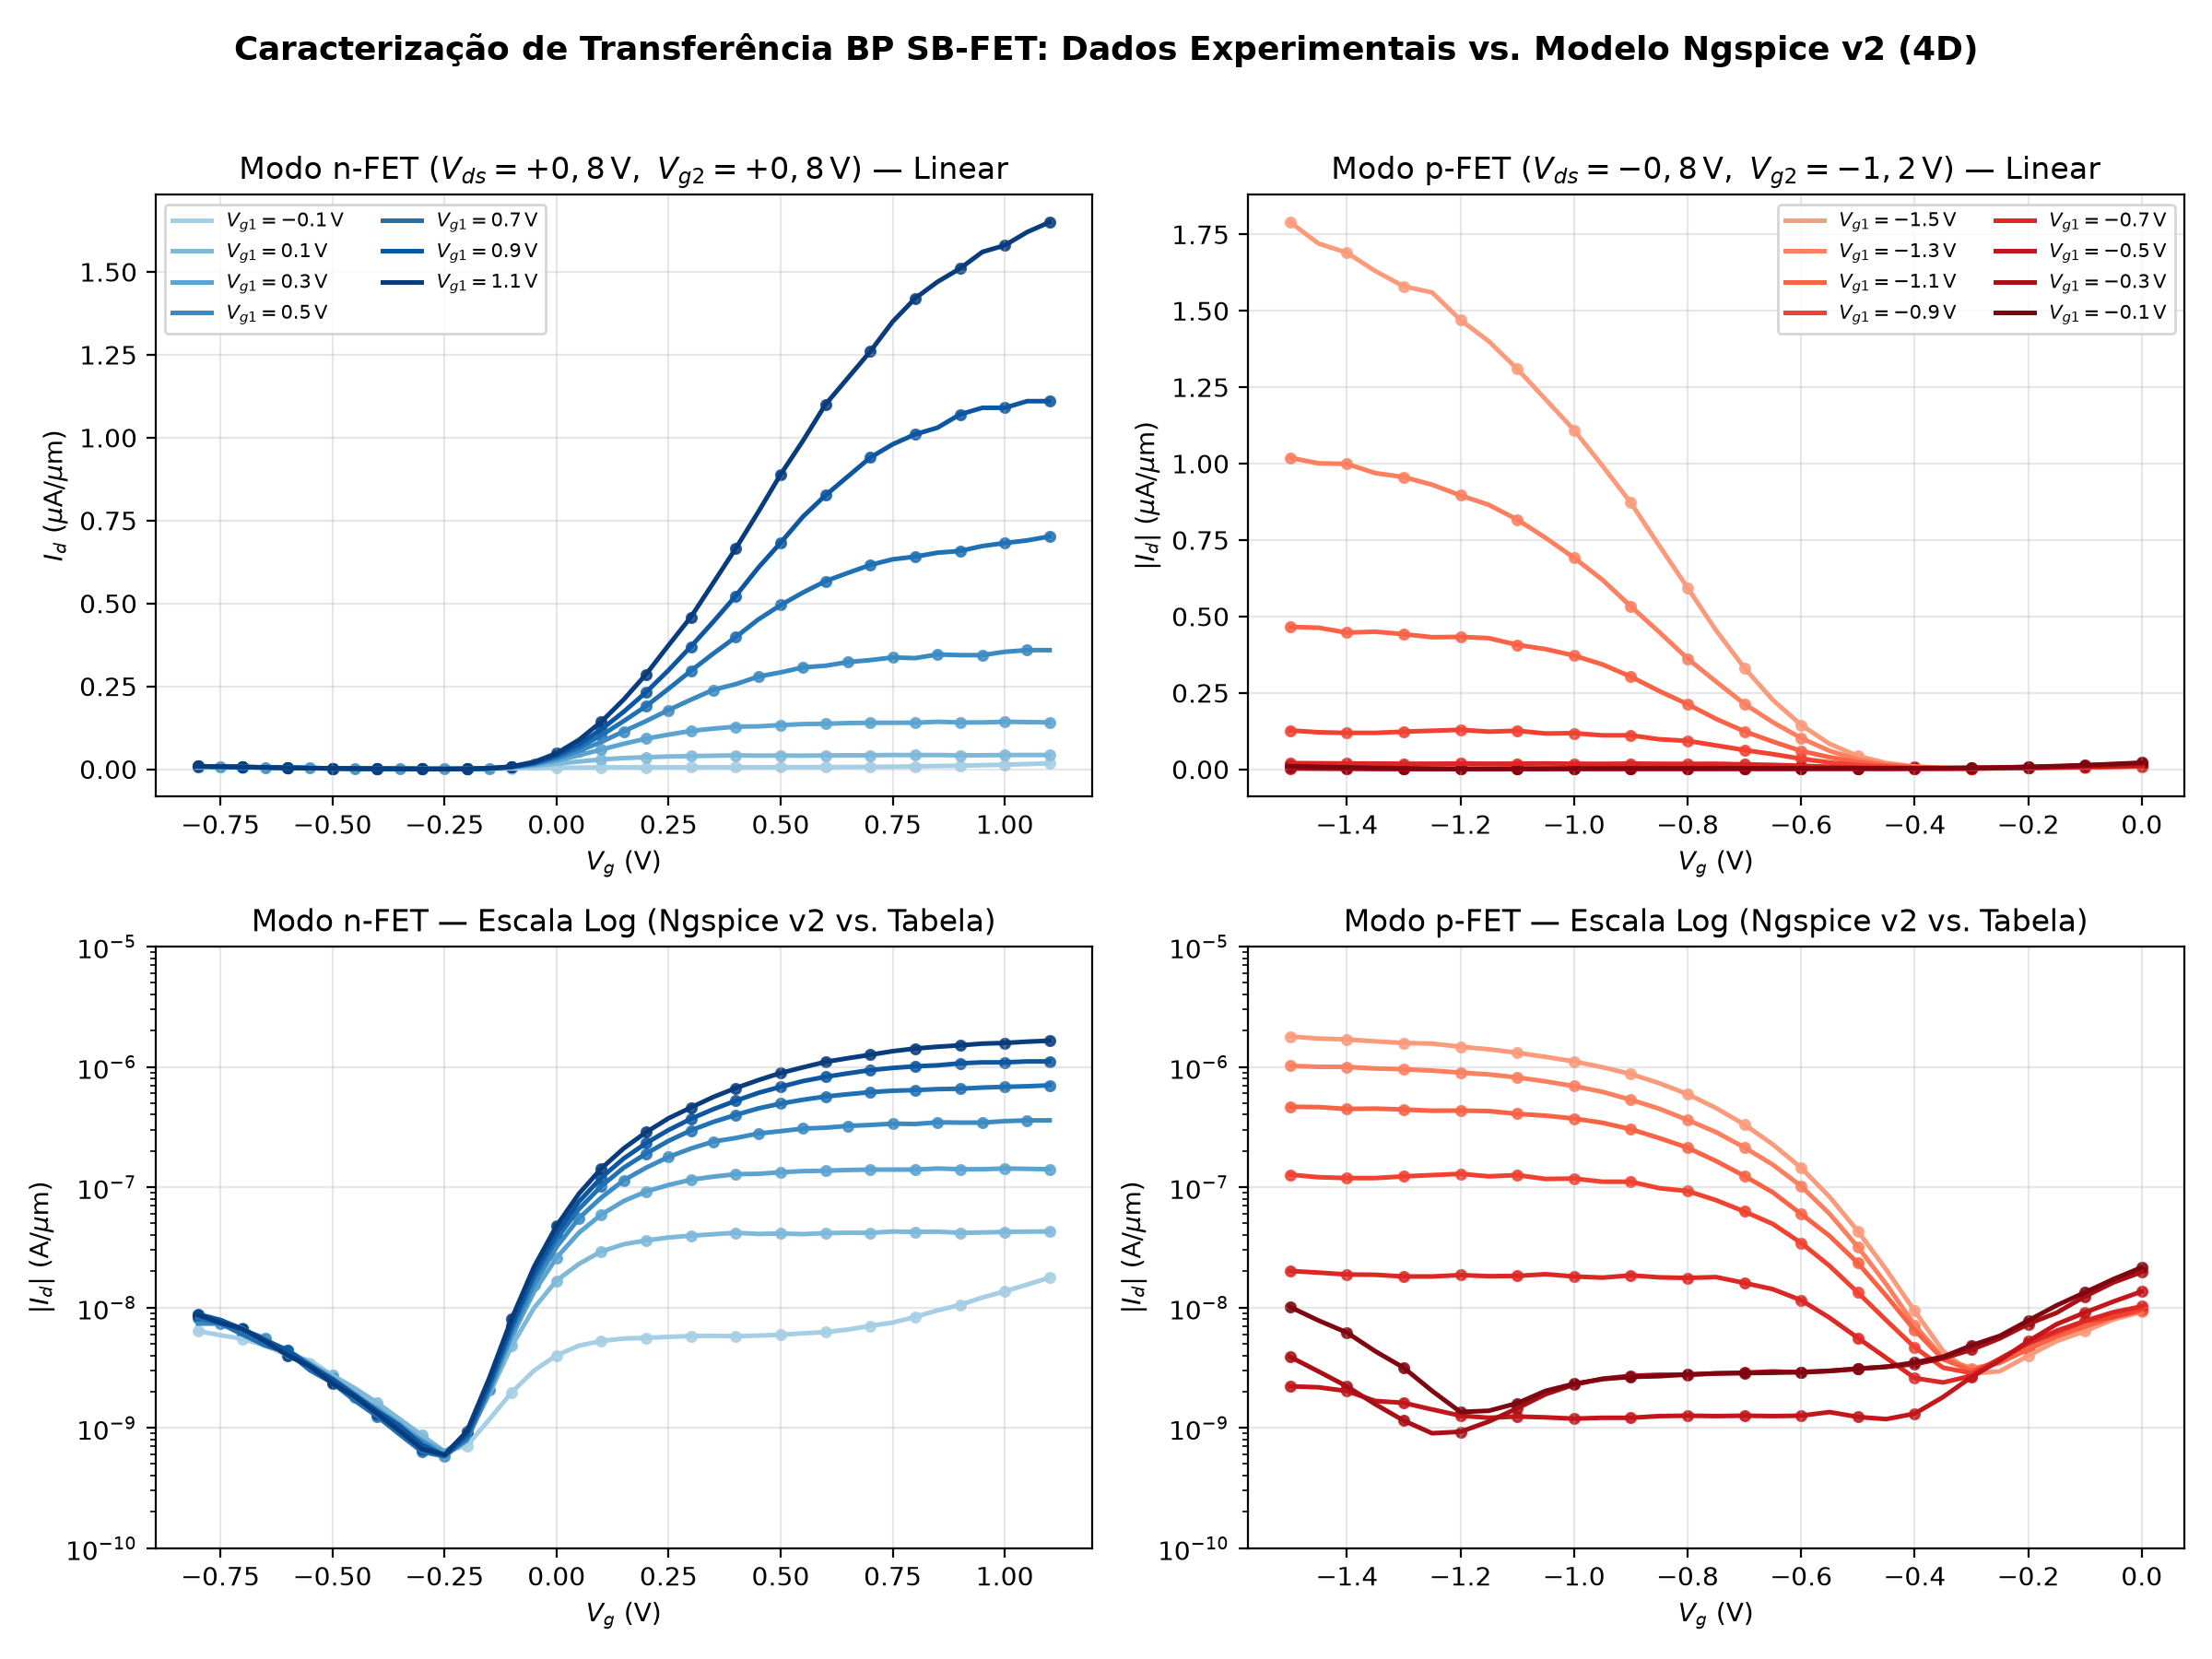
\includegraphics[width=0.92\textwidth]{m00_transfer_NP_log_lin.png}
\caption{Linear and logarithmic transfer curves ($I_d \times V_g$) simulated in \texttt{ngspice-47} against experimental data points for \textit{n-FET} and \textit{p-FET} modes.}
\label{fig:m00_transfer}
\end{figure}

\begin{figure}[htbp]
\centering
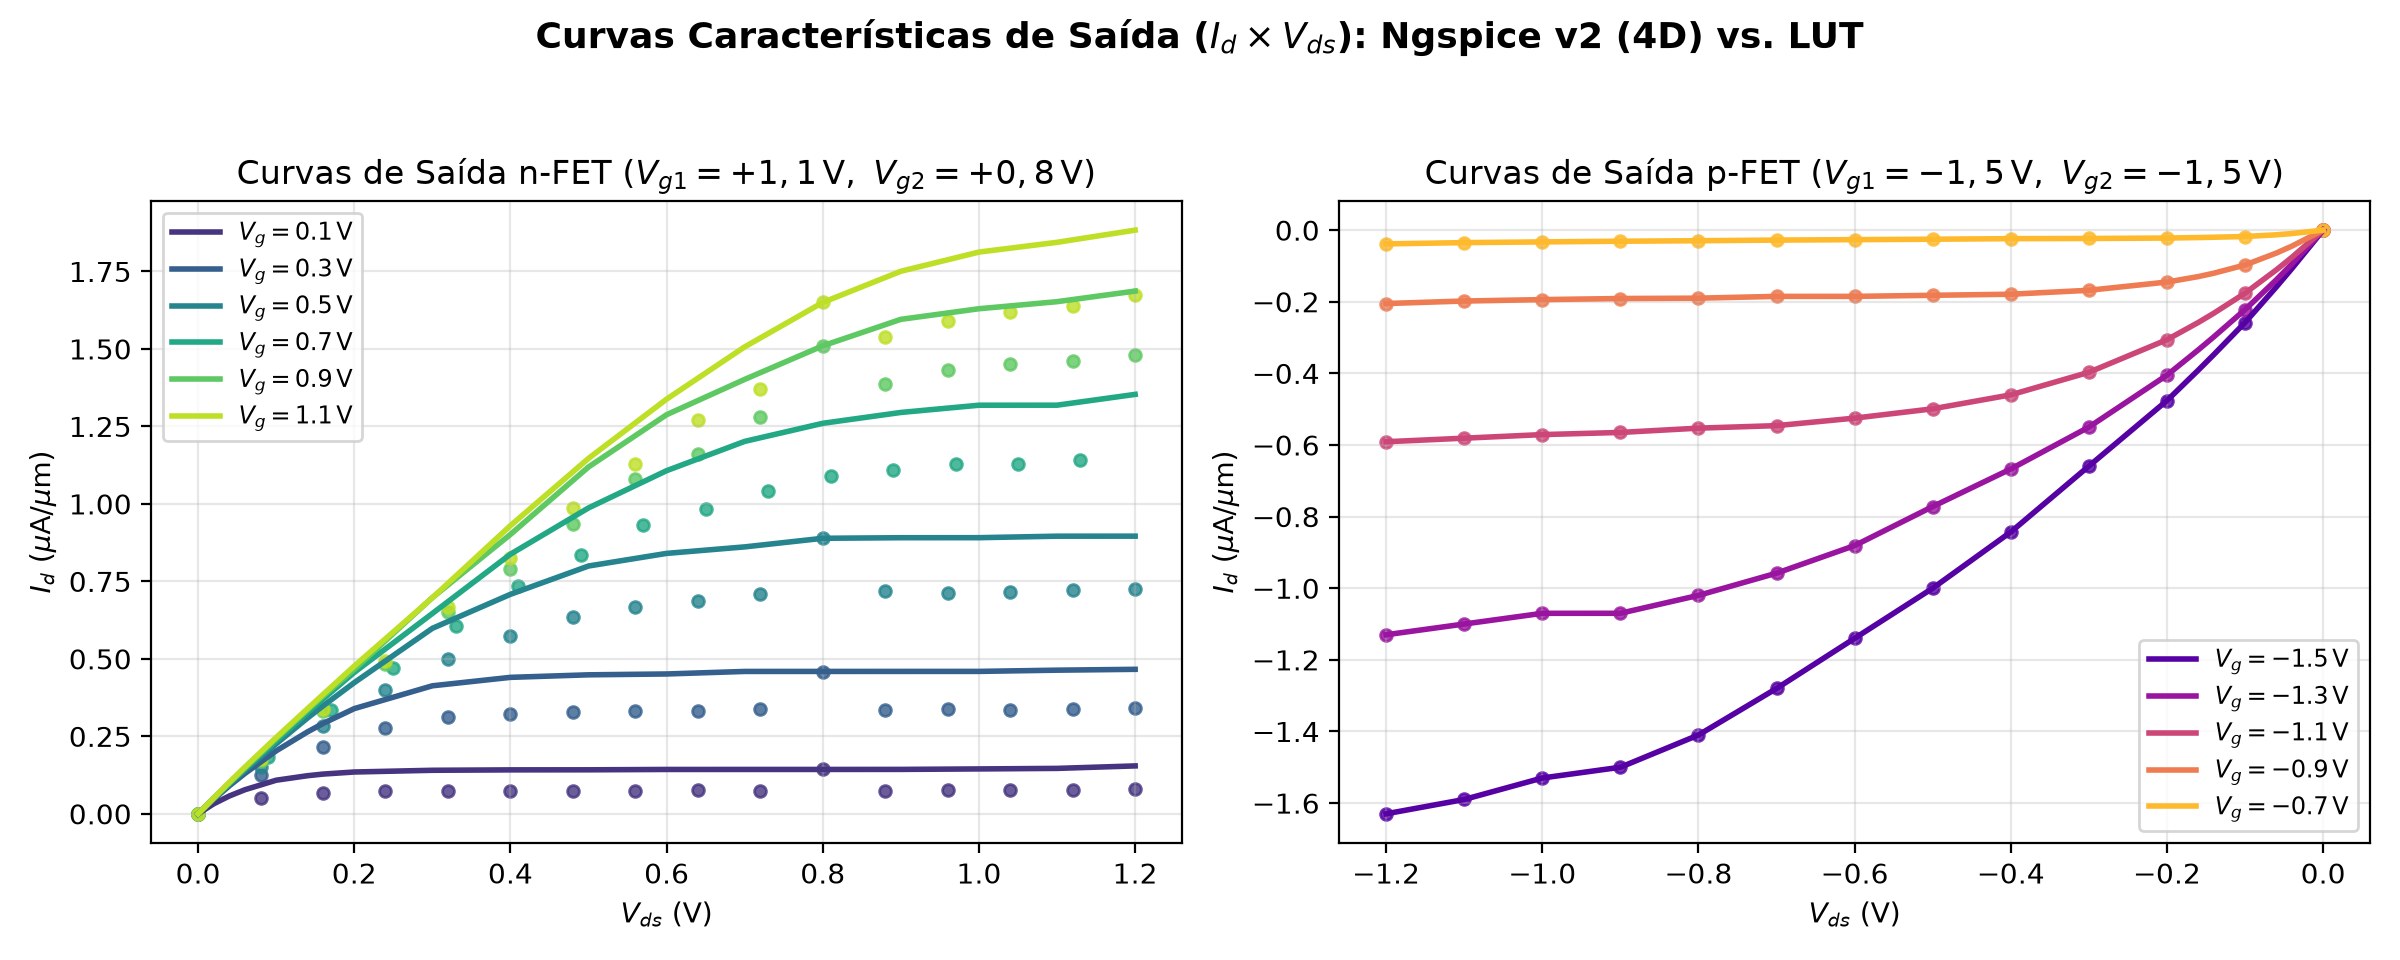
\includegraphics[width=0.92\textwidth]{m00_output_NP.png}
\caption{Output characteristic families ($I_d \times V_{ds}$) in \textit{n-FET} ($V_{ds}>0$) and \textit{p-FET} ($V_{ds}<0$, $V_{g2}=-1.5\ \text{V}$) regimes capturing gate-dependent triode-to-saturation transitions.}
\label{fig:m00_output}
\end{figure}

\begin{figure}[htbp]
\centering
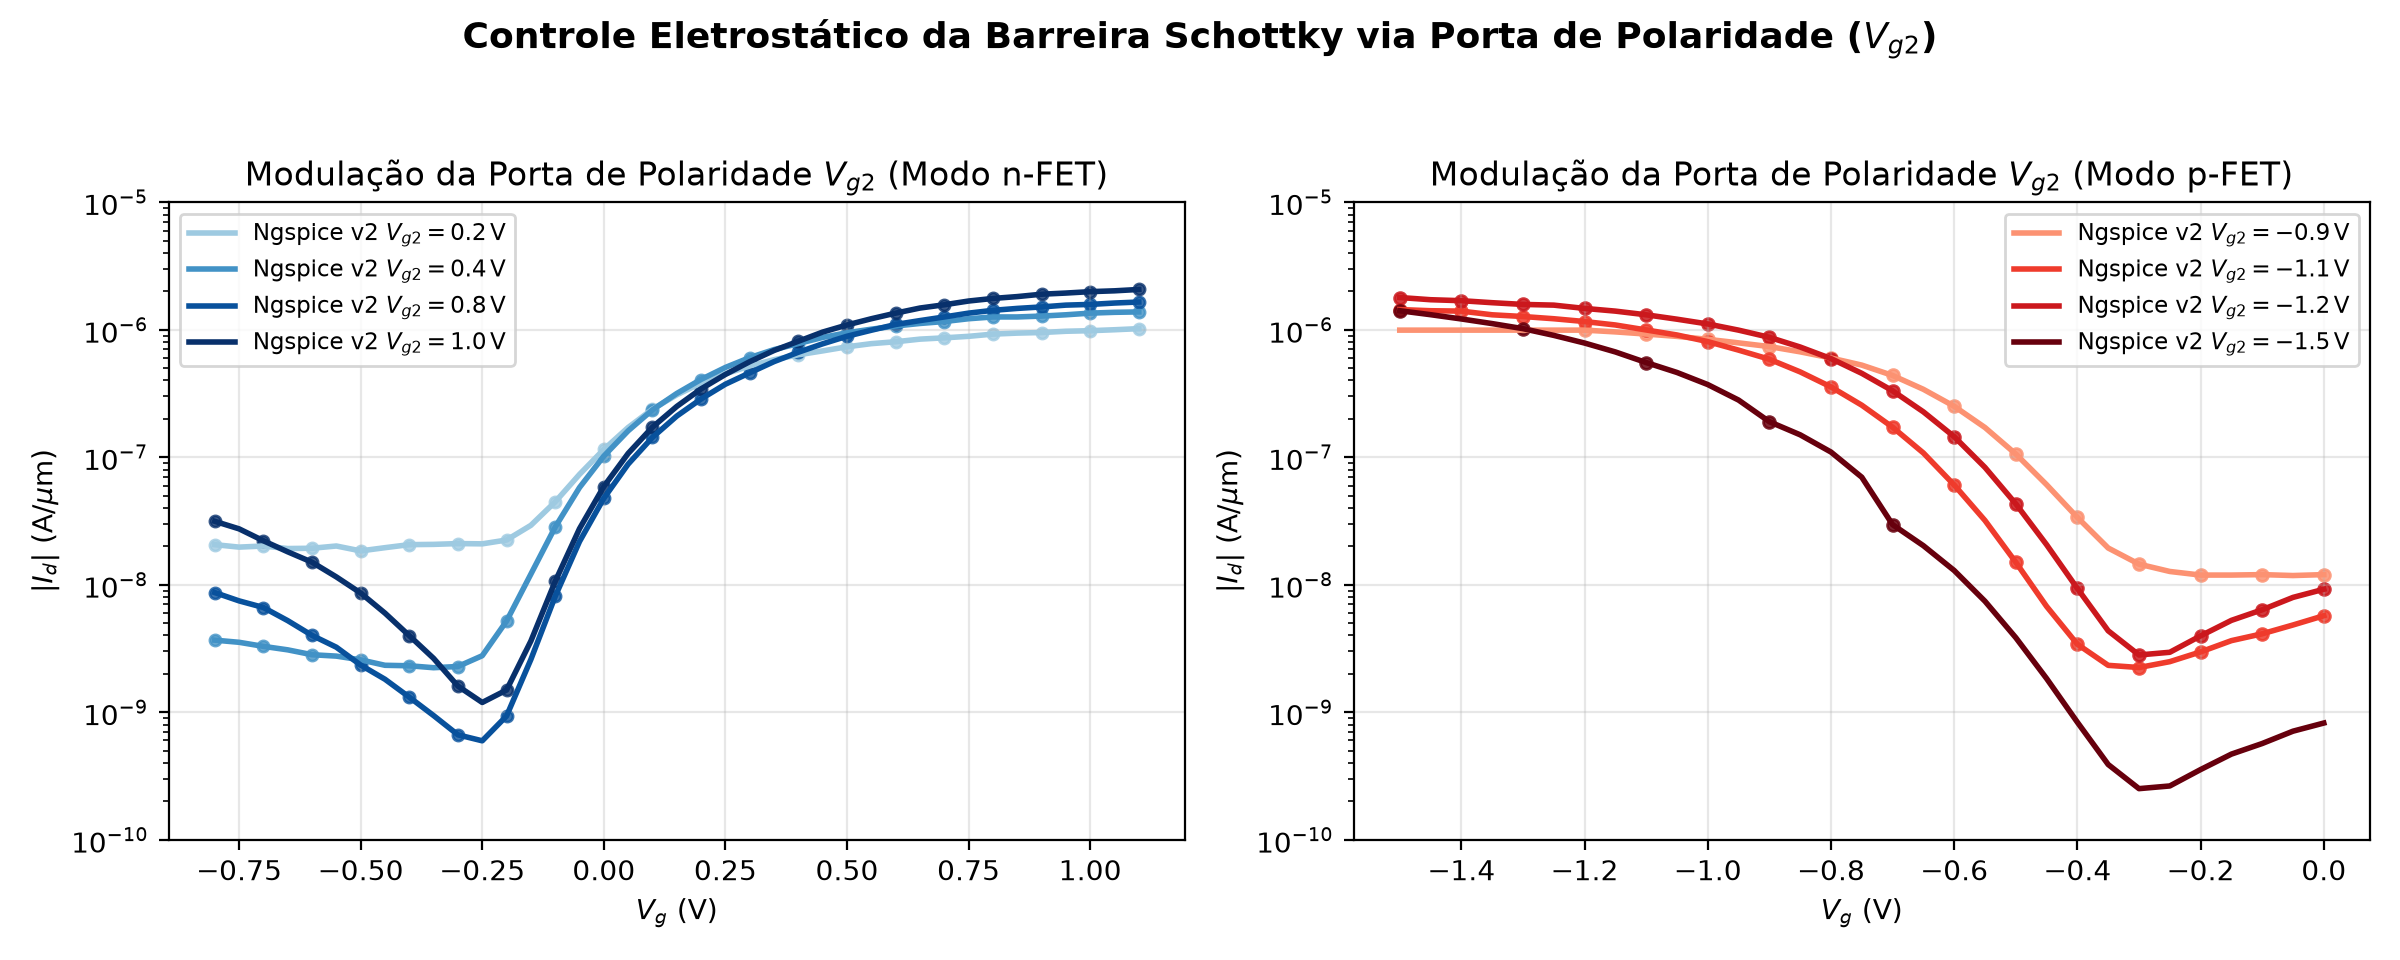
\includegraphics[width=0.92\textwidth]{m00_efeito_porta_polaridade.png}
\caption{Electrostatic modulation of channel current by the polarity gate $V_{g2}$ in \textit{n-FET} and \textit{p-FET} modes, highlighting the flat-band shift at $V_{g2}=-1.5\ \text{V}$.}
\label{fig:m00_pg}
\end{figure}

\begin{figure}[htbp]
\centering
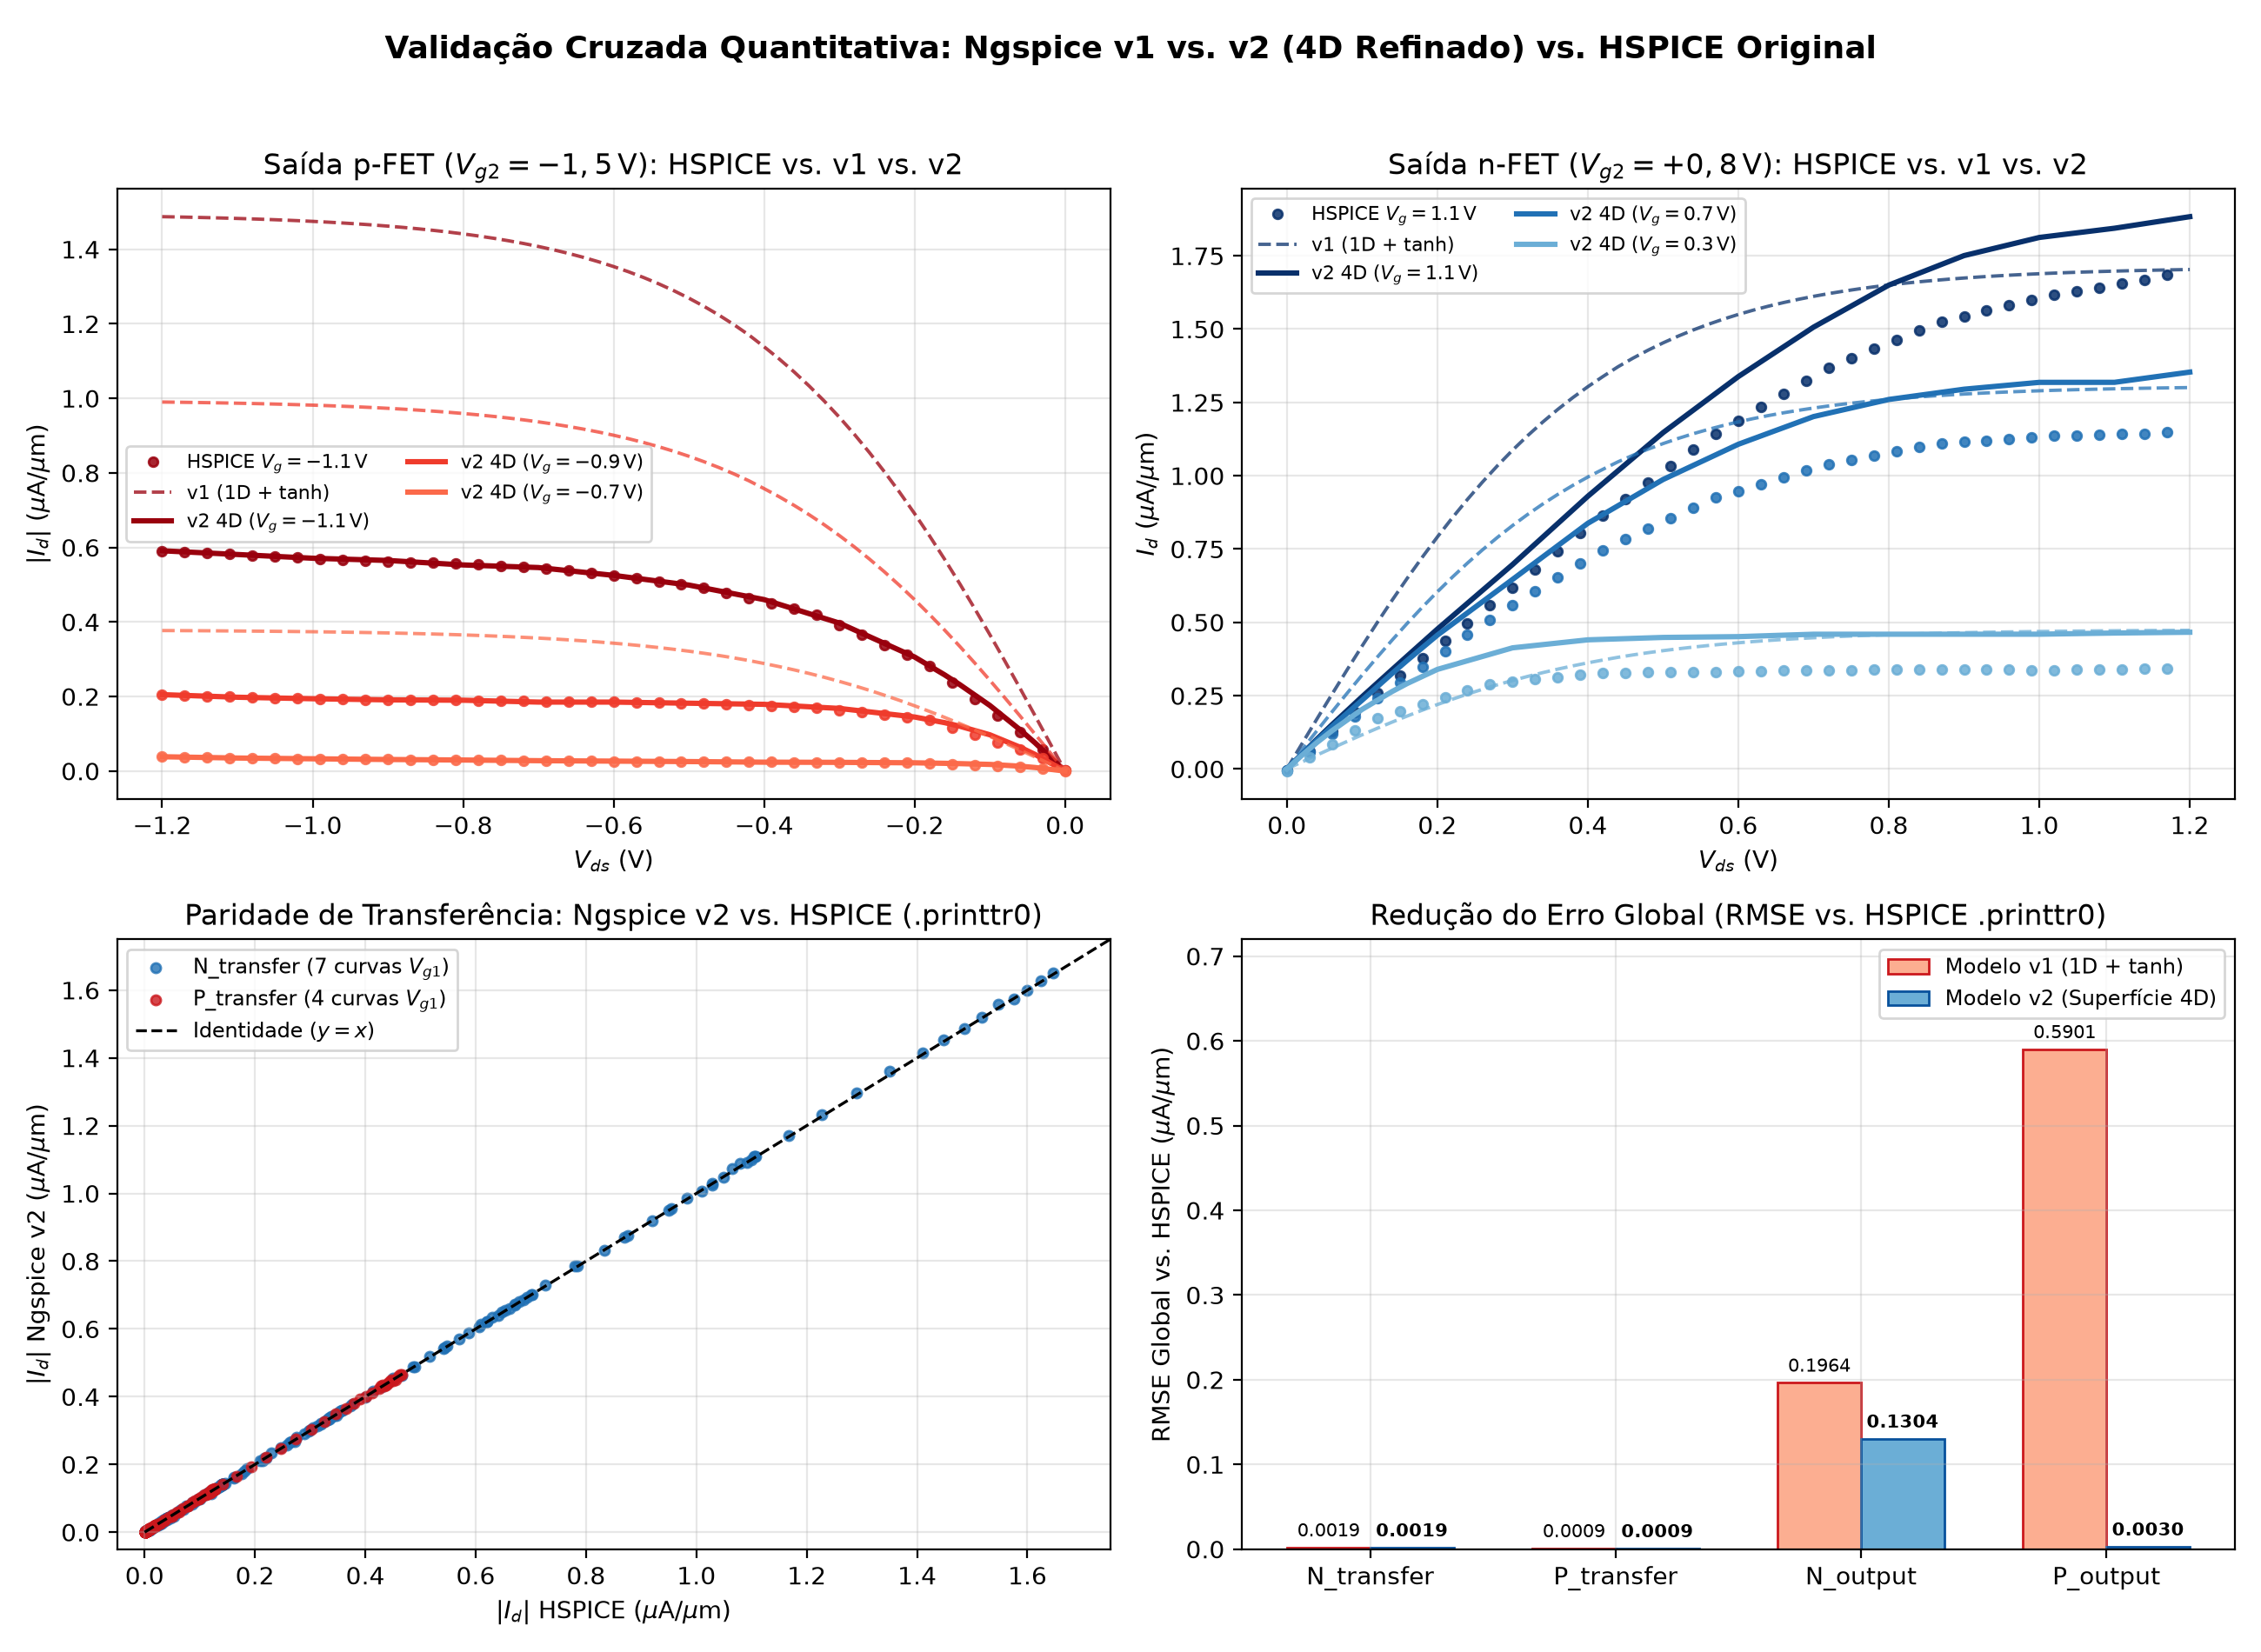
\includegraphics[width=0.92\textwidth]{m00_validacao_cruzada_hspice.png}
\caption{Quantitative cross-validation comparing the preliminary model (\texttt{v1}), the refined 4D model (\texttt{v2}) in \texttt{ngspice-47}, and the reference Synopsys HSPICE \texttt{.printtr0} traces.}
\label{fig:m00_hspice}
\end{figure}

\subsection{Ultra-Low-Voltage Complementary Inverter}\label{sec:res_inverter}

Static performance metrics of the complementary BP SB-FET inverter from $V_{DD} = 1.0\ \text{V}$ down to $0.2\ \text{V}$ are compiled in Table~\ref{tab:inverter_vtc}. Without $V_{fb}$ compensation (direct coupling), threshold misalignment between the \textit{p-FET} and \textit{n-FET} branches shifts the switching threshold $V_M$ toward $0\ \text{V}$, collapsing inverter functionality for $V_{DD} \le 0.4\ \text{V}$ ($2.77\%$ swing and $|A_v|_{\max} = 0.37$ at $0.4\ \text{V}$; $1.27\%$ swing and $0.06$ gain at $0.2\ \text{V}$).

\begin{table}[htbp]
\centering
\caption{Static metrics of the complementary BP SB-FET inverter under $V_{DD}$ scaling ($1.0\ \text{V}$ to $0.2\ \text{V}$).}
\label{tab:inverter_vtc}
\resizebox{\textwidth}{!}{%
\begin{tabular}{l c c c c c c c c}
\toprule
\textbf{Configuration} & $V_{DD}$ (V) & $V_{\mathrm{out}}(0)$ (V) & $V_{\mathrm{out}}(V_{DD})$ (V) & \textbf{Swing (\%)} & $V_M$ (V) & $|A_v|_{\max}$ & $NM_L$ (V) & $NM_H$ (V) \\
\midrule
Direct (No $V_{fb}$ comp.) & $1.0$ & $0.991$ & $0.004$ & $98.67\%$ & $0.278$ & $22.03$ & $0.096$ & $0.564$ \\
Direct (No $V_{fb}$ comp.) & $0.8$ & $0.788$ & $0.004$ & $98.12\%$ & $0.162$ & $39.32$ & $0.034$ & $0.537$ \\
Direct (No $V_{fb}$ comp.) & $0.6$ & $0.559$ & $0.003$ & $92.68\%$ & $0.066$ & $37.24$ & $0.000$ & $0.475$ \\
Direct (No $V_{fb}$ comp.) & $0.4$ & $0.014$ & $0.003$ & $2.77\%$  & $0.010$ & $0.37$  & $0.000$ & $0.000$ \\
Direct (No $V_{fb}$ comp.) & $0.2$ & $0.005$ & $0.003$ & $1.27\%$  & $0.006$ & $0.06$  & $0.000$ & $0.000$ \\
\midrule
Compensated ($V_{fb}$ aligned) & $1.0$ & $0.999$ & $0.003$ & $99.63\%$ & $0.540$ & $54.69$ & $0.461$ & $0.373$ \\
Compensated ($V_{fb}$ aligned) & $0.8$ & $0.800$ & $0.002$ & $99.75\%$ & $0.438$ & $50.84$ & $0.362$ & $0.278$ \\
Compensated ($V_{fb}$ aligned) & $0.6$ & $0.600$ & $0.001$ & $99.80\%$ & $0.336$ & $38.18$ & $0.266$ & $0.178$ \\
Compensated ($V_{fb}$ aligned) & $0.4$ & $0.400$ & $0.003$ & $99.29\%$ & $0.234$ & $12.71$ & $0.172$ & $0.076$ \\
Compensated ($V_{fb}$ aligned) & $0.2$ & $0.198$ & $0.018$ & $89.75\%$ & $0.126$ & $2.71$  & $0.080$ & $0.000$ \\
\bottomrule
\end{tabular}}
\end{table}

With electrostatic $V_{fb}$ alignment, $V_M$ centers near $V_{DD}/2$ (Figure~\ref{fig:m01_vtc}), sustaining over $99.2\%$ output swing down to $0.4\ \text{V}$ and reaching peak voltage gains of $|A_v|_{\max} = 54.69$ ($1.0\ \text{V}$) and $38.18$ ($0.6\ \text{V}$). Even at the extreme ultra-low-voltage regime ($V_{DD} = 0.2\ \text{V}$), the inverter maintains $89.75\%$ rail-to-rail swing and differential gain $2.71 > 1$, satisfying the criterion for logic regeneration. In transient switching under $C_{\mathrm{load}} = 0.5\ \text{fF}$ (Figure~\ref{fig:m01_tran}), transitions complete on the nanosecond scale with nanoampere static leakage and dynamic current peaks of $1.28\ \mu\text{A}$ at $1.0\ \text{V}$ and $0.73\ \mu\text{A}$ at $0.6\ \text{V}$.

\begin{figure}[htbp]
\centering
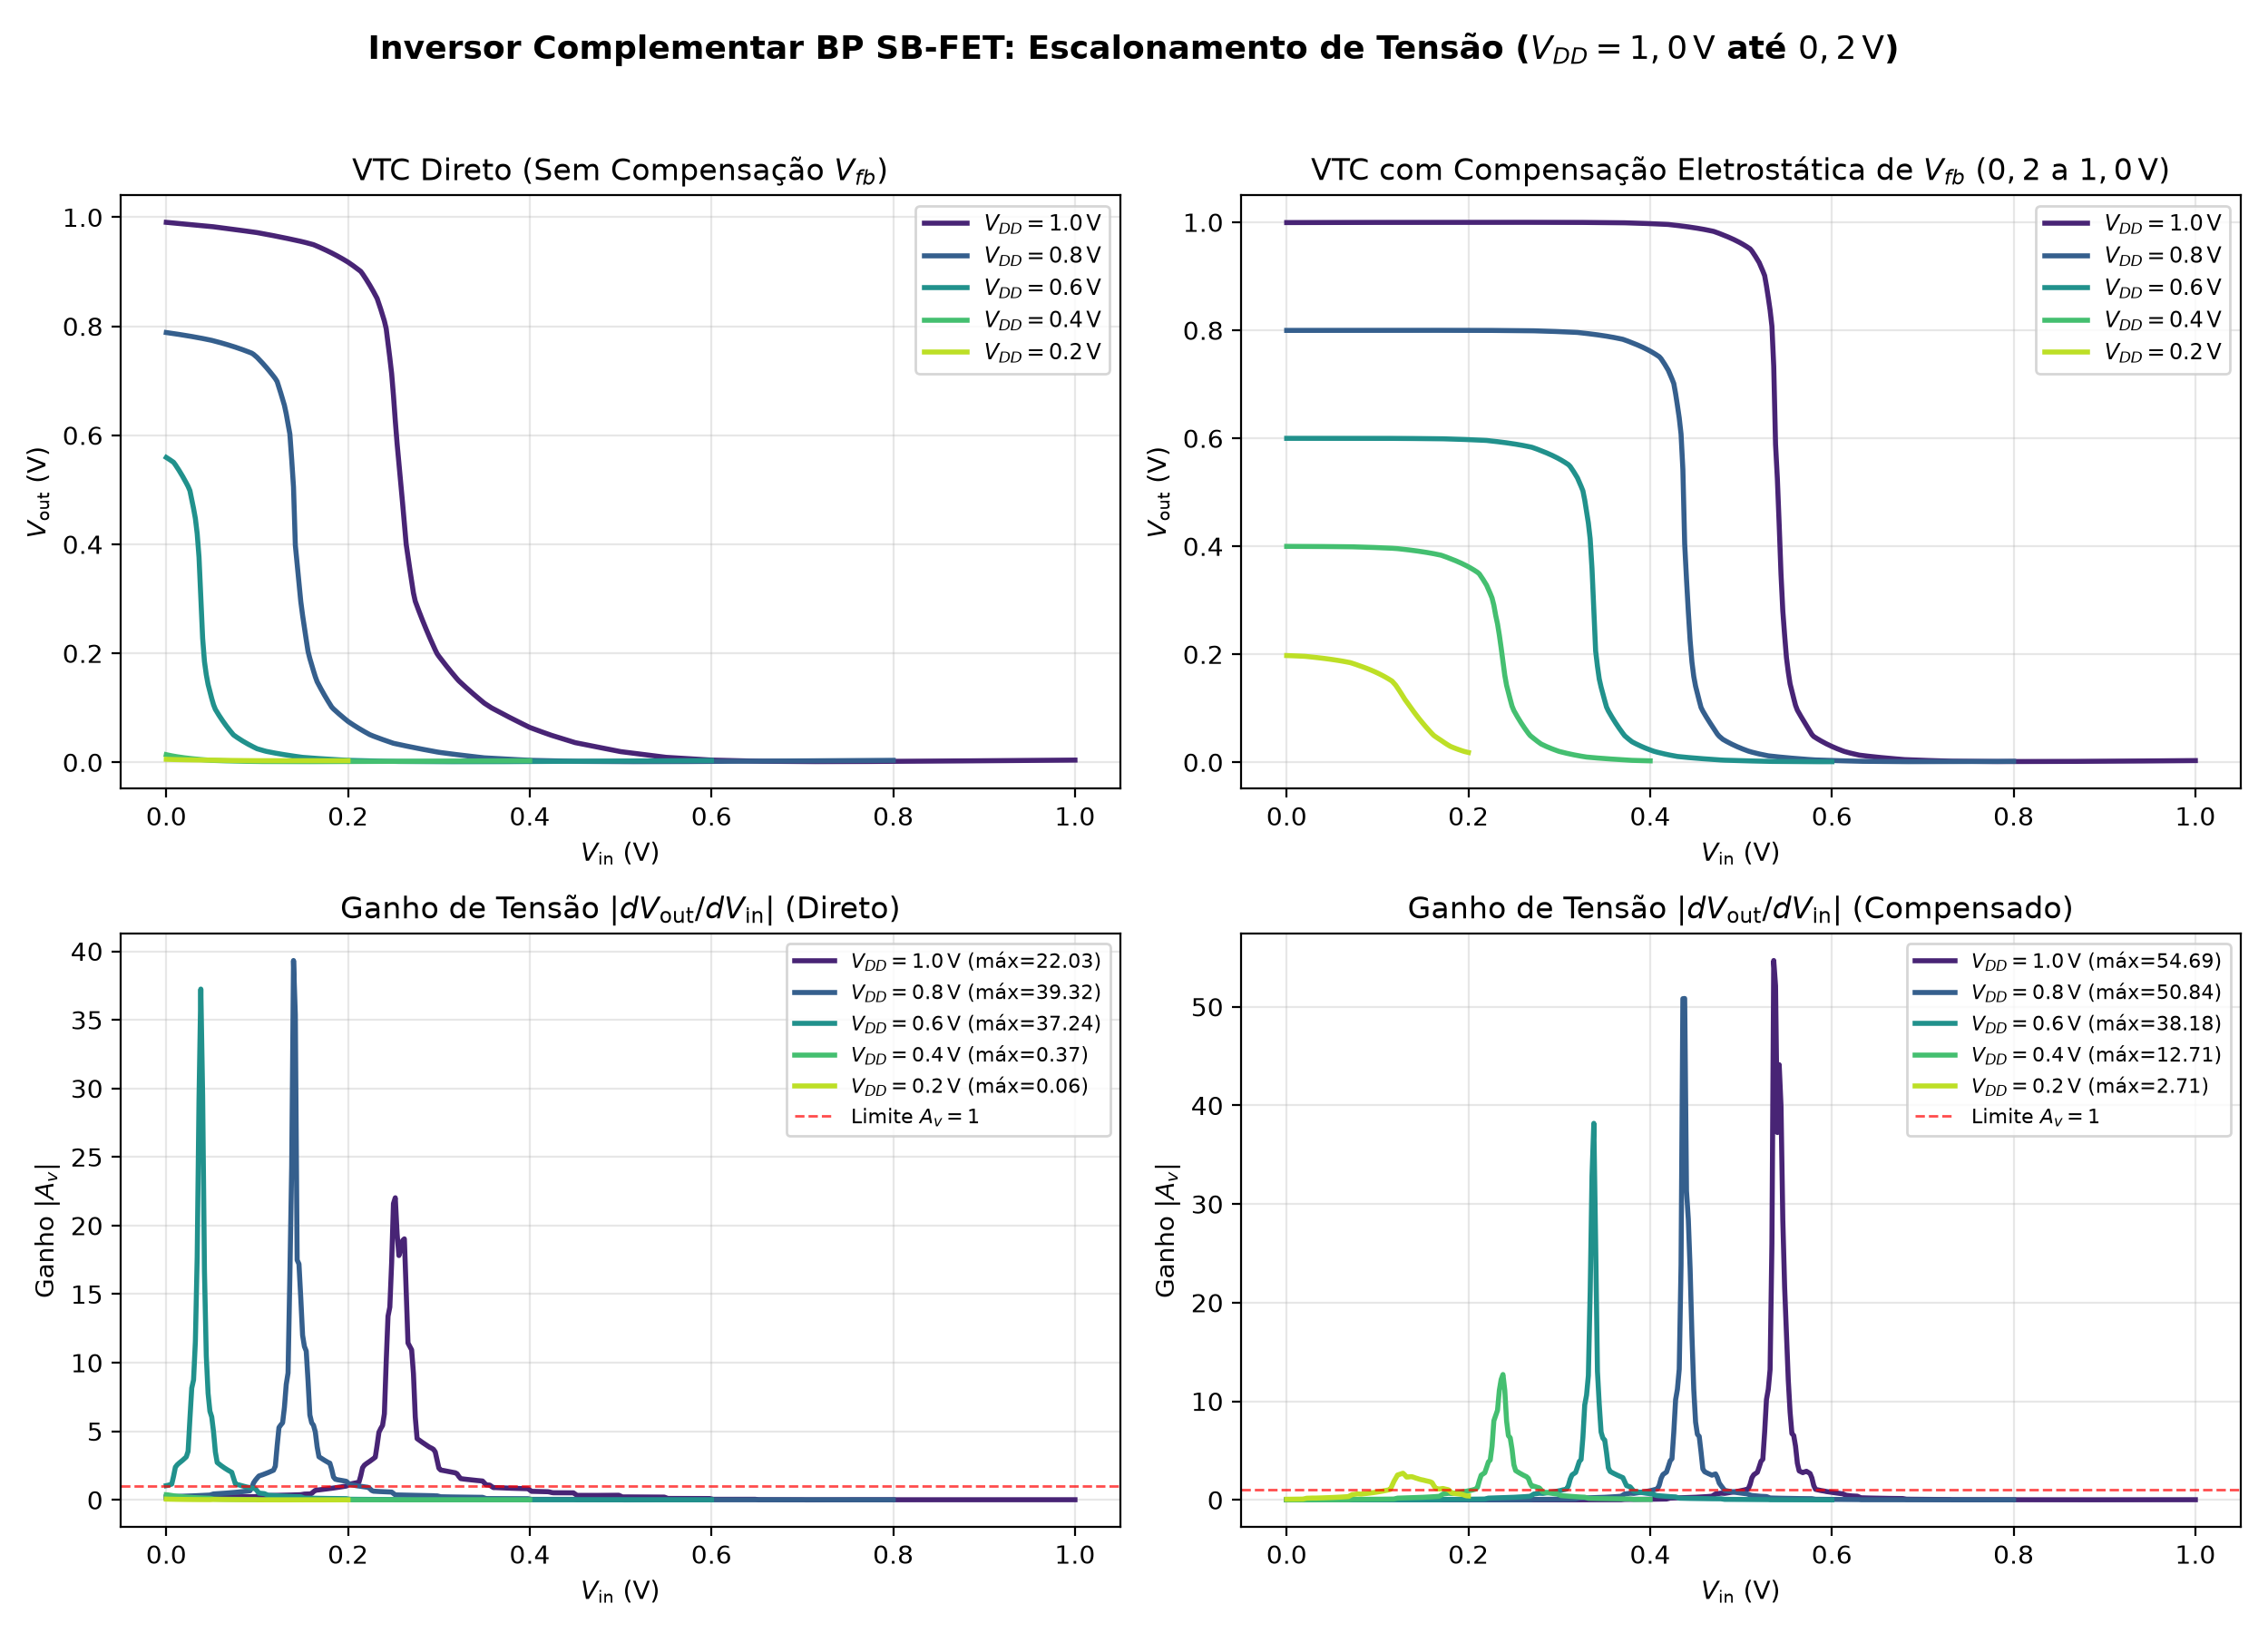
\includegraphics[width=0.92\textwidth]{m01_inversor_vtc_ganho.png}
\caption{Voltage transfer characteristics (VTC) and differential gain $|dV_{\mathrm{out}}/dV_{\mathrm{in}}|$ of the BP SB-FET inverter without compensation (left) and with $V_{fb}$ alignment (right) from $1.0\ \text{V}$ to $0.2\ \text{V}$.}
\label{fig:m01_vtc}
\end{figure}

\begin{figure}[htbp]
\centering
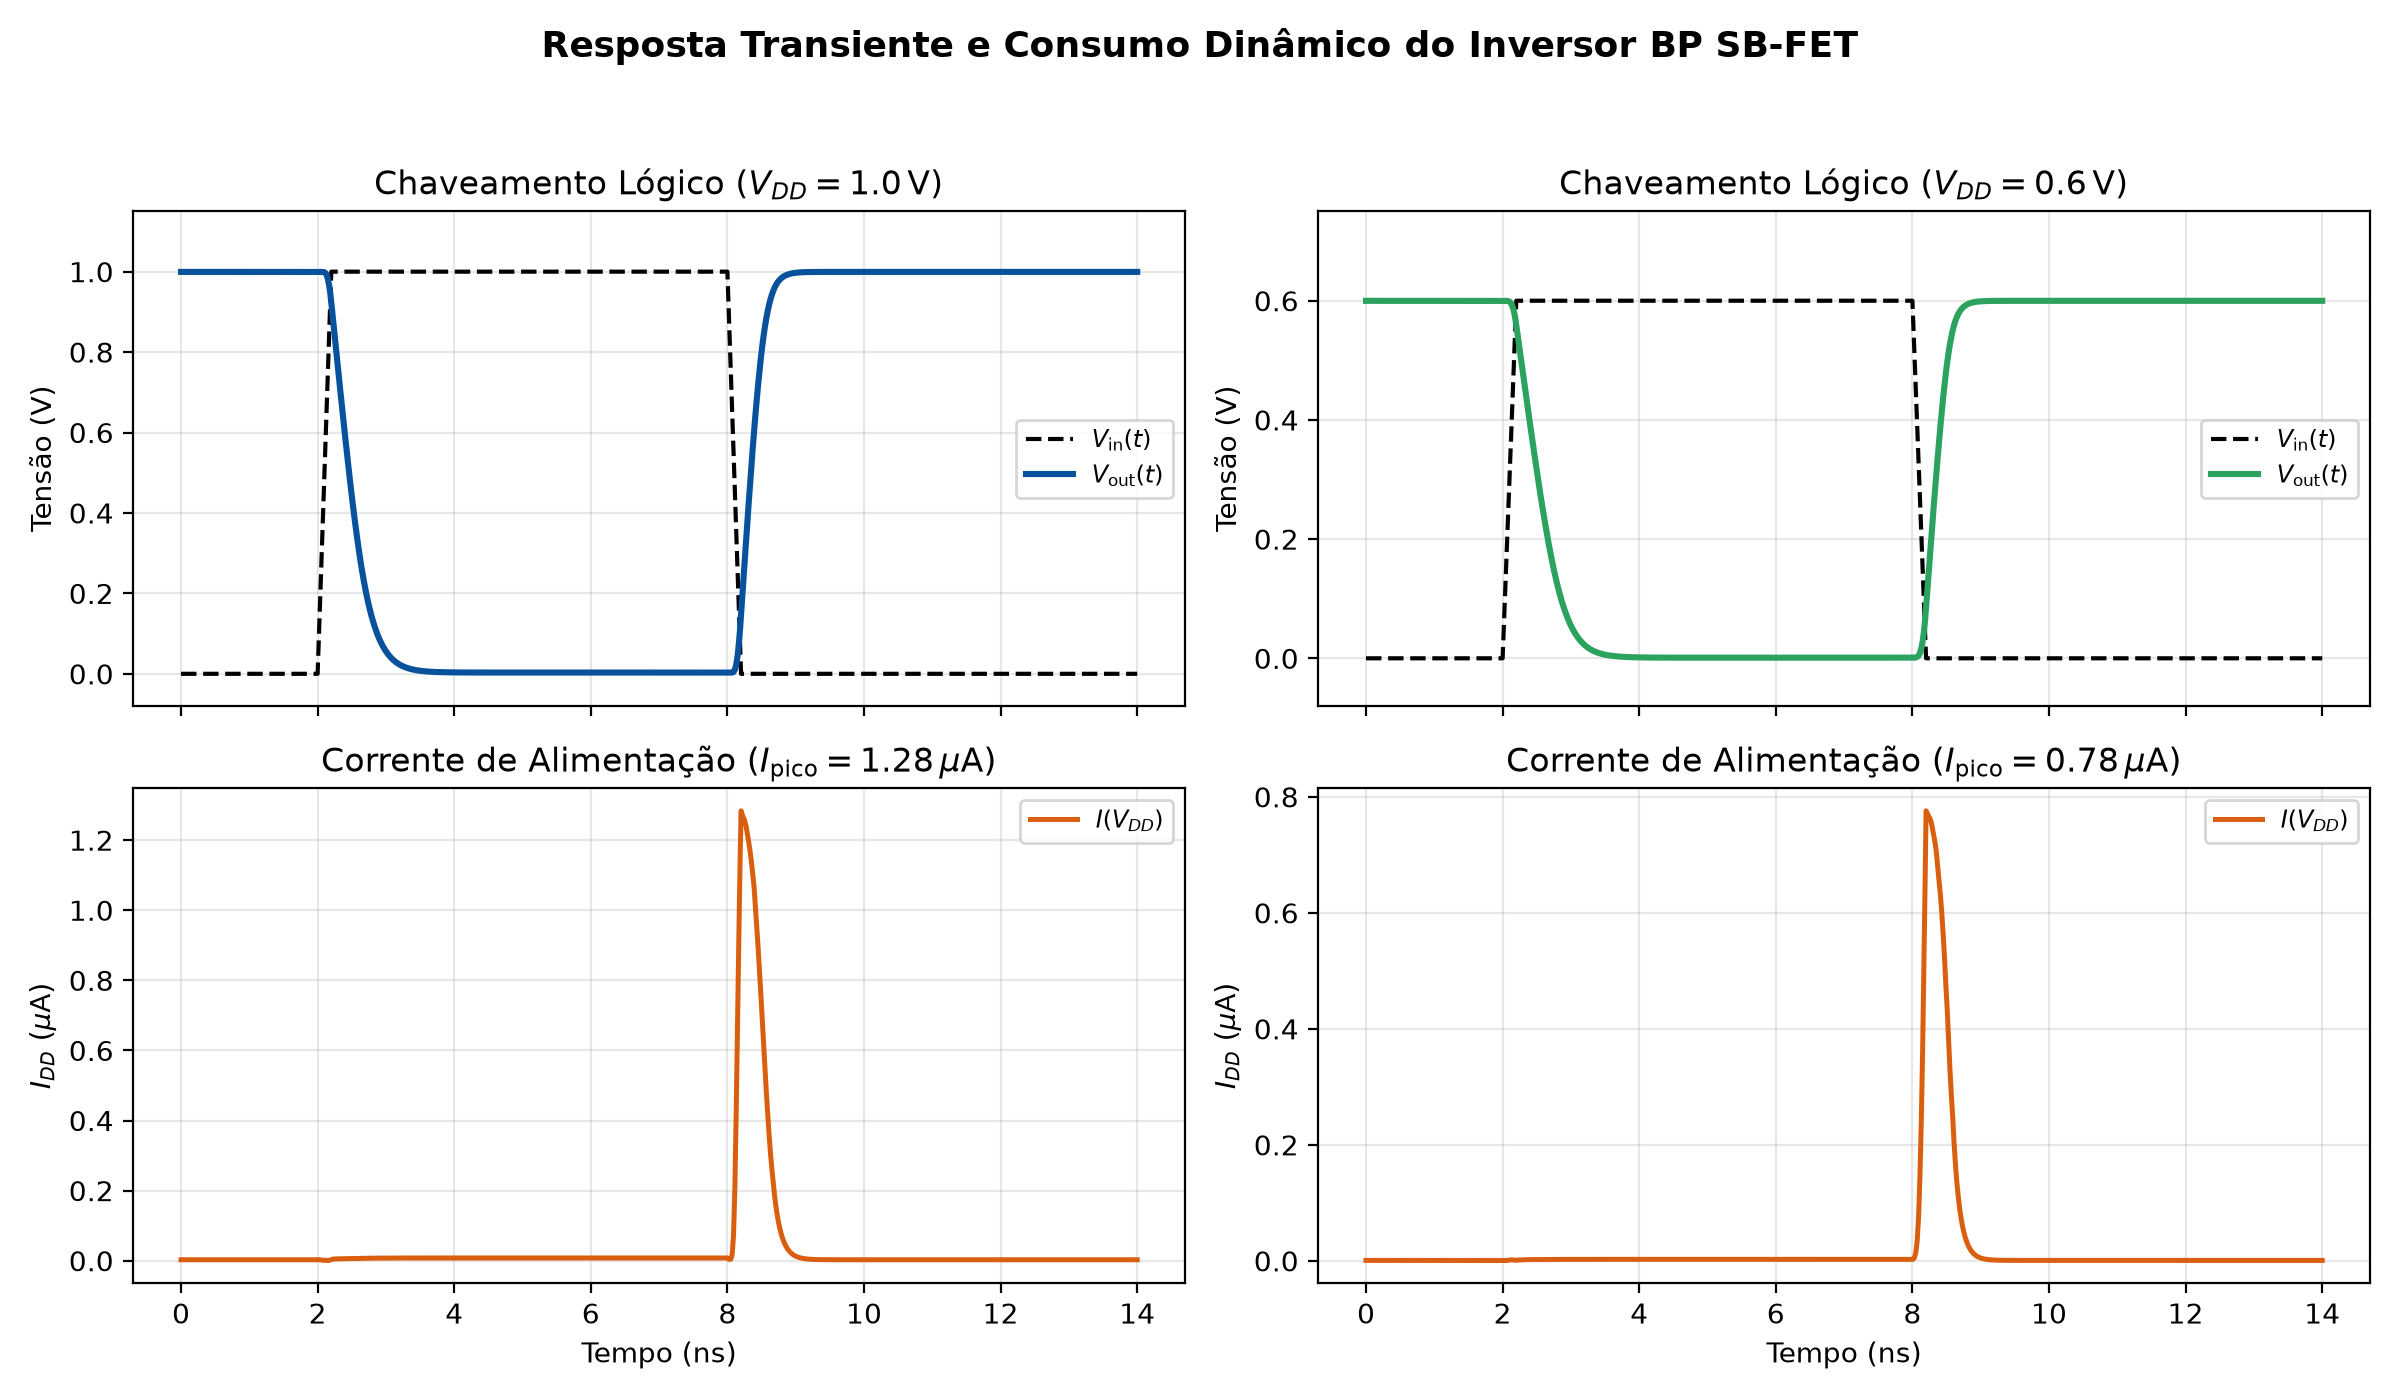
\includegraphics[width=0.90\textwidth]{m01_inversor_transiente.png}
\caption{Transient switching response ($C_{\mathrm{load}} = 0.5\ \text{fF}$) and dynamic supply current peaks $I(V_{DD})$ of the compensated inverter at $V_{DD} = 1.0\ \text{V}$ and $0.6\ \text{V}$.}
\label{fig:m01_tran}
\end{figure}

\subsection{Dynamic Polymorphic Logic Gates (\texttt{NAND}/\texttt{NOR} and \texttt{XOR}/\texttt{XNOR})}\label{sec:res_poly}

The $40\ \text{ns}$ transient simulations verified $100\%$ Boolean accuracy ($16/16$ input-key combinations) across both 4-transistor polymorphic primitives with zero transistor overhead, as detailed in Table~\ref{tab:polymorphic_gates}. In the \texttt{NAND}/\texttt{NOR} cell ($V_{DD}=0.8\ \text{V}$), logic \texttt{'1'} outputs range between $0.701\ \text{V}$ and $0.790\ \text{V}$, while logic \texttt{'0'} outputs remain below $0.013\ \text{V}$. In the \texttt{XOR}/\texttt{XNOR} bridge ($V_{DD}=1.5\ \text{V}$, $V_{\mathrm{in}}=1.1\ \text{V}$), all \texttt{'1'} states settle at $1.465\ \text{V}$ and all \texttt{'0'} states settle at $0.002\ \text{V}$.

\begin{table}[htbp]
\centering
\caption{Electrical truth table and peak currents measured in \texttt{ngspice-47} for the 4T polymorphic gates.}
\label{tab:polymorphic_gates}
\footnotesize
\begin{tabular}{l c c c c c c c}
\toprule
\textbf{Gate ($V_{DD}$)} & \textbf{Key} & \textbf{Function} & $(A,B)$ & $V_{\mathrm{out}}$ (V) & \textbf{Meas.\ Bit} & \textbf{Exp.\ Bit} & $I_{\mathrm{peak}}$ ($\mu\text{A}$) \\
\midrule
\texttt{NAND}/\texttt{NOR} ($0.8\ \text{V}$) & $\text{Key}=0$ & \texttt{NAND} & \texttt{00} & $0.790$ & \texttt{1} & \texttt{1} & $0.041$ \\
\texttt{NAND}/\texttt{NOR} ($0.8\ \text{V}$) & $\text{Key}=0$ & \texttt{NAND} & \texttt{01} & $0.762$ & \texttt{1} & \texttt{1} & $0.182$ \\
\texttt{NAND}/\texttt{NOR} ($0.8\ \text{V}$) & $\text{Key}=0$ & \texttt{NAND} & \texttt{10} & $0.769$ & \texttt{1} & \texttt{1} & $0.390$ \\
\texttt{NAND}/\texttt{NOR} ($0.8\ \text{V}$) & $\text{Key}=0$ & \texttt{NAND} & \texttt{11} & $0.013$ & \texttt{0} & \texttt{0} & $0.589$ \\
\texttt{NAND}/\texttt{NOR} ($0.8\ \text{V}$) & $\text{Key}=1$ & \texttt{NOR}  & \texttt{00} & $0.701$ & \texttt{1} & \texttt{1} & $0.213$ \\
\texttt{NAND}/\texttt{NOR} ($0.8\ \text{V}$) & $\text{Key}=1$ & \texttt{NOR}  & \texttt{01} & $0.001$ & \texttt{0} & \texttt{0} & $0.716$ \\
\texttt{NAND}/\texttt{NOR} ($0.8\ \text{V}$) & $\text{Key}=1$ & \texttt{NOR}  & \texttt{10} & $0.004$ & \texttt{0} & \texttt{0} & $0.092$ \\
\texttt{NAND}/\texttt{NOR} ($0.8\ \text{V}$) & $\text{Key}=1$ & \texttt{NOR}  & \texttt{11} & $0.001$ & \texttt{0} & \texttt{0} & $0.006$ \\
\midrule
\texttt{XOR}/\texttt{XNOR} ($1.5\ \text{V}$) & $\text{Key}=0$ & \texttt{XOR}  & \texttt{00} & $0.002$ & \texttt{0} & \texttt{0} & $0.004$ \\
\texttt{XOR}/\texttt{XNOR} ($1.5\ \text{V}$) & $\text{Key}=0$ & \texttt{XOR}  & \texttt{01} & $1.465$ & \texttt{1} & \texttt{1} & $1.691$ \\
\texttt{XOR}/\texttt{XNOR} ($1.5\ \text{V}$) & $\text{Key}=0$ & \texttt{XOR}  & \texttt{10} & $1.465$ & \texttt{1} & \texttt{1} & $0.366$ \\
\texttt{XOR}/\texttt{XNOR} ($1.5\ \text{V}$) & $\text{Key}=0$ & \texttt{XOR}  & \texttt{11} & $0.002$ & \texttt{0} & \texttt{0} & $1.903$ \\
\texttt{XOR}/\texttt{XNOR} ($1.5\ \text{V}$) & $\text{Key}=1$ & \texttt{XNOR} & \texttt{00} & $1.465$ & \texttt{1} & \texttt{1} & $1.699$ \\
\texttt{XOR}/\texttt{XNOR} ($1.5\ \text{V}$) & $\text{Key}=1$ & \texttt{XNOR} & \texttt{01} & $0.002$ & \texttt{0} & \texttt{0} & $1.908$ \\
\texttt{XOR}/\texttt{XNOR} ($1.5\ \text{V}$) & $\text{Key}=1$ & \texttt{XNOR} & \texttt{10} & $0.002$ & \texttt{0} & \texttt{0} & $0.032$ \\
\texttt{XOR}/\texttt{XNOR} ($1.5\ \text{V}$) & $\text{Key}=1$ & \texttt{XNOR} & \texttt{11} & $1.465$ & \texttt{1} & \texttt{1} & $1.691$ \\
\bottomrule
\end{tabular}
\end{table}

Figures~\ref{fig:m02_nand_nor} and \ref{fig:m02_xor_xnor} demonstrate instantaneous functional transmutation at $t = 20\ \text{ns}$ and highlight a key structural contrast: whereas \texttt{NAND}/\texttt{NOR} displays current peaks strongly governed by which series or parallel network drives the transition, the \texttt{XOR}/\texttt{XNOR} bridge exhibits nearly identical charging ($\approx 1.69\ \mu\text{A}$) and discharging ($\approx 1.90\text{--}1.91\ \mu\text{A}$) peaks across both key configurations.

\begin{figure}[htbp]
\centering
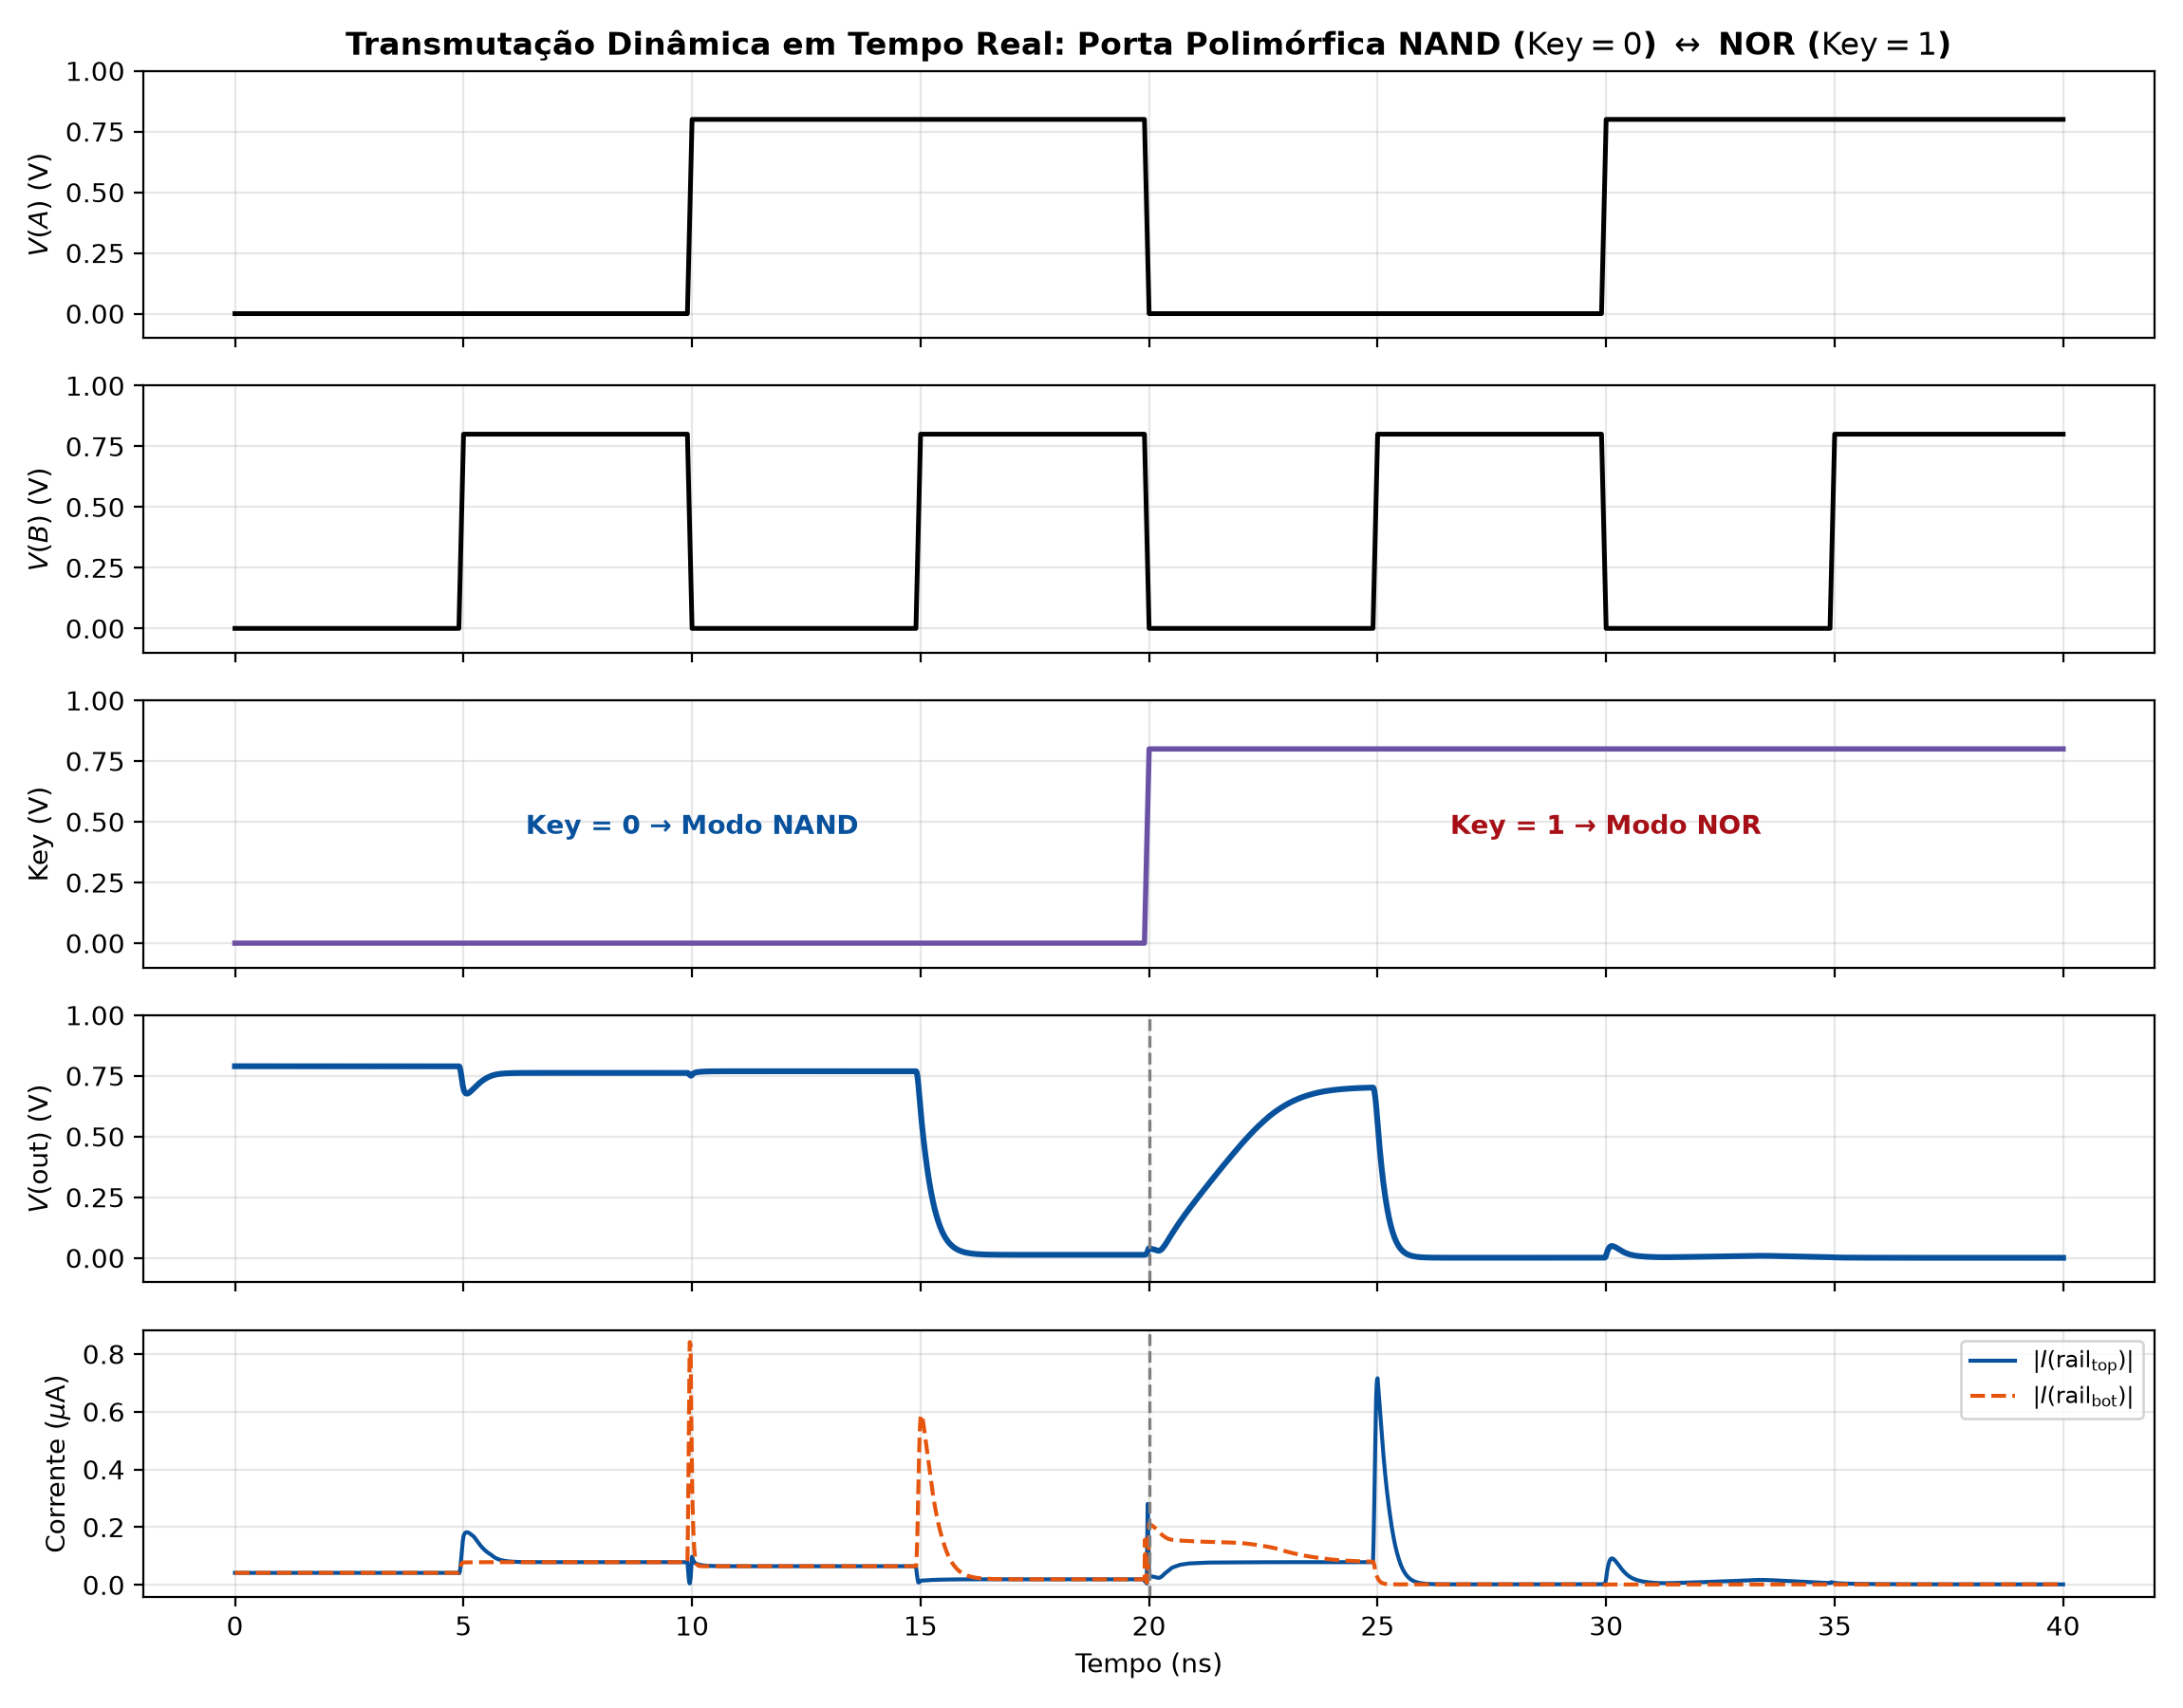
\includegraphics[width=0.90\textwidth]{m02_nand_nor_dinamico.png}
\caption{Dynamic switching \texttt{NAND} ($\text{Key}=0$) $\leftrightarrow$ \texttt{NOR} ($\text{Key}=1$) at $V_{DD} = 0.8\ \text{V}$ and its asymmetric supply current profile.}
\label{fig:m02_nand_nor}
\end{figure}

\begin{figure}[htbp]
\centering
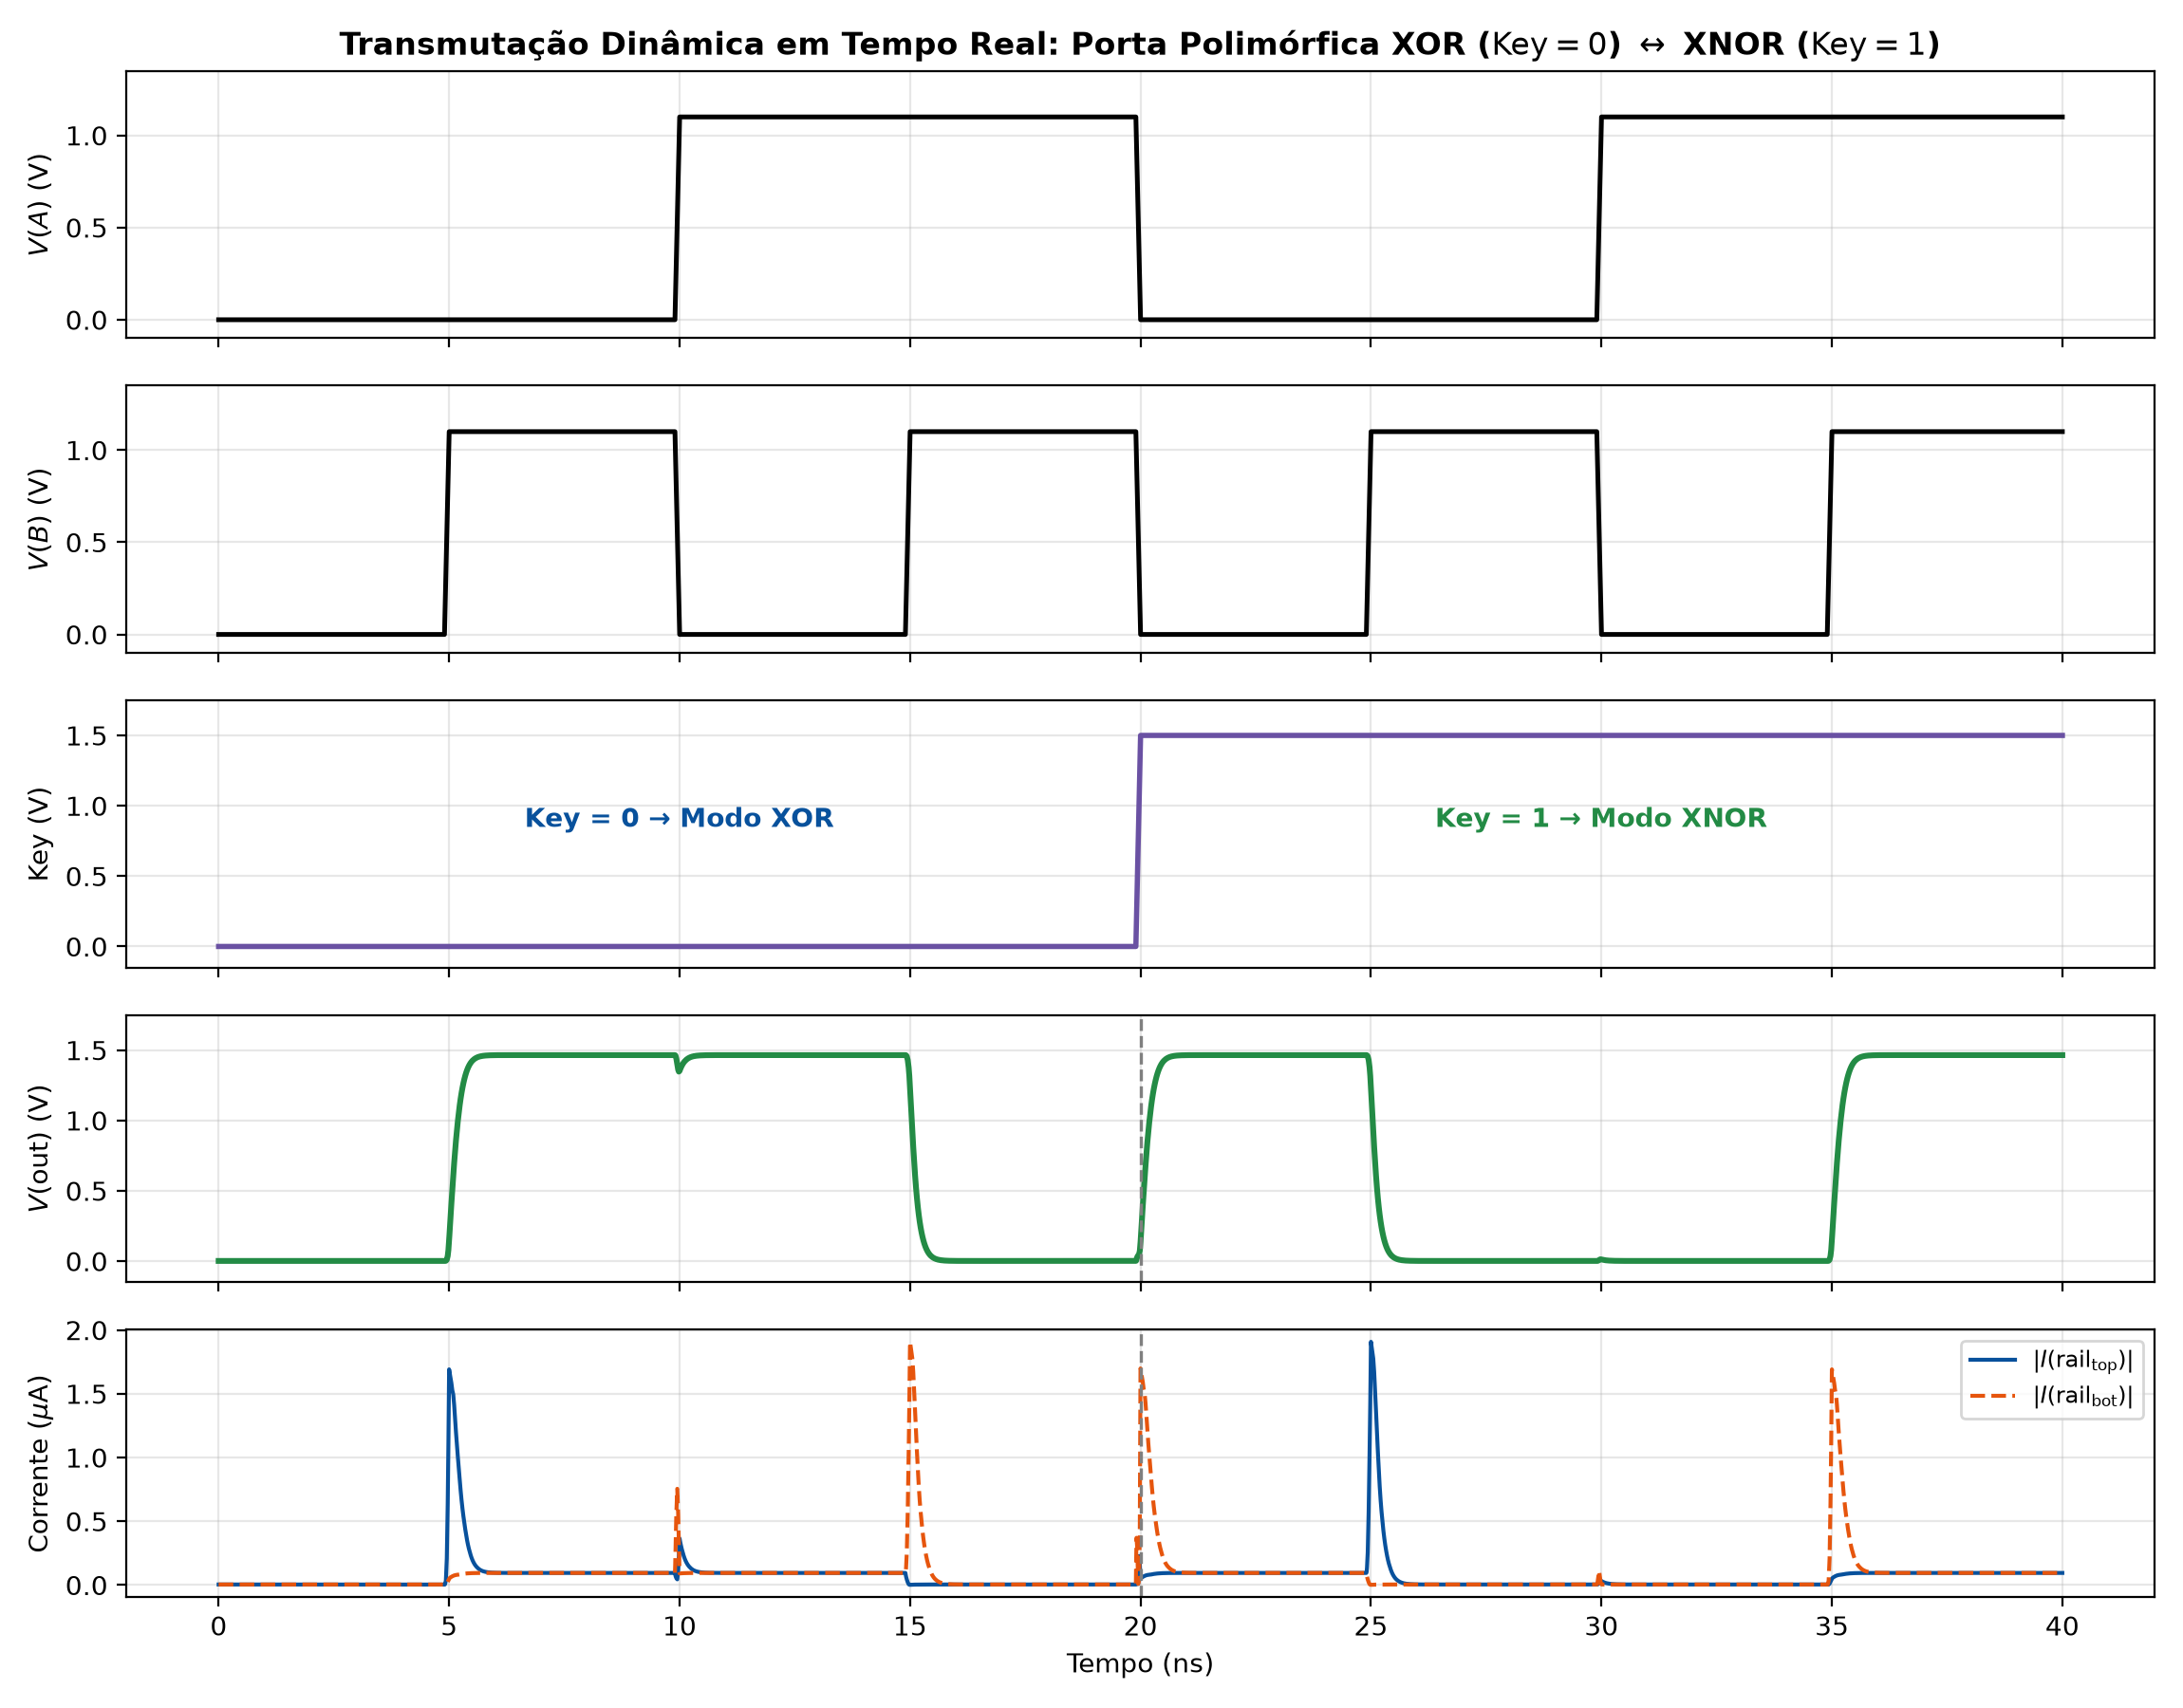
\includegraphics[width=0.90\textwidth]{m02_xor_xnor_dinamico.png}
\caption{Dynamic switching \texttt{XOR} ($\text{Key}=0$) $\leftrightarrow$ \texttt{XNOR} ($\text{Key}=1$) at $V_{DD} = 1.5\ \text{V}$ showing symmetric complementary switching current peaks.}
\label{fig:m02_xor_xnor}
\end{figure}

\subsection{Side-Channel Security (DPA), 3D Robustness, and Floating Retention}\label{sec:res_dpa_mc}

The Python port of the reference waveform datasets~\cite{wu2020reconfigurable} (Table~\ref{tab:dpa_mc_m03} and Figure~\ref{fig:m03_dpa}) confirms that the \texttt{NAND}/\texttt{NOR} family exhibits a $50.35\%$ peak current discrepancy ($2.15\ \mu\text{A}$ vs.\ $1.43\ \mu\text{A}$) and moderate temporal correlation ($r = 0.515$), whereas \texttt{XOR}/\texttt{XNOR} suppresses peak disparity to just $0.56\%$ ($1.80\ \mu\text{A}$ vs.\ $1.79\ \mu\text{A}$), concealing the active key state against side-channel inspection.

\begin{table}[htbp]
\centering
\caption{DPA signature metrics and Monte Carlo statistical robustness ($N=250$ samples/gate) from Module~\texttt{03}.}
\label{tab:dpa_mc_m03}
\begin{subtable}{\textwidth}
\centering
\caption{Comparison of supply current signatures $|I(V_{DD})|$ across modes (\texttt{metricas\_dpa.csv}).}
\footnotesize
\begin{tabular}{l c c c c c c}
\toprule
\textbf{Family} & $I_{\mathrm{peak},0}$ ($\mu\text{A}$) & $I_{\mathrm{peak},1}$ ($\mu\text{A}$) & \textbf{Peak Diff.\ (\%)} & $I_{\mathrm{avg},0}$ ($\mu\text{A}$) & $I_{\mathrm{avg},1}$ ($\mu\text{A}$) & \textbf{Correlation} $r$ \\
\midrule
\texttt{NAND}/\texttt{NOR} & $2.15$ & $1.43$ & $50.35\%$ & $0.212$ & $0.163$ & $+0.515$ \\
\texttt{XOR}/\texttt{XNOR} & $1.80$ & $1.79$ & $0.56\%$  & $0.267$ & $0.230$ & $-0.114$ \\
\bottomrule
\end{tabular}
\end{subtable}

\vspace{0.8em}

\begin{subtable}{\textwidth}
\centering
\caption{Logic separation statistics under simultaneous $V_{DD}$ and $V_{SS}$ noise (\texttt{metricas\_seguranca\_robustez.csv}).}
\footnotesize
\begin{tabular}{l c c c c c c}
\toprule
\textbf{Gate} & \textbf{Samples} & $\mu(V_{\text{`1'}})$ (V) & $\sigma(V_{\text{`1'}})$ (mV) & $\mu(V_{\text{`0'}})$ (V) & $\sigma(V_{\text{`0'}})$ (mV) & \textbf{Logic Accuracy} \\
\midrule
\texttt{NAND} & $250$ & $0.793$ & $126.55$ & $0.038$ & $106.50$ & $100.0\%$ \\
\texttt{NOR}  & $250$ & $0.770$ & $118.01$ & $0.015$ & $101.47$ & $100.0\%$ \\
\texttt{XOR}  & $250$ & $0.782$ & $122.80$ & $0.006$ & $89.23$  & $100.0\%$ \\
\texttt{XNOR} & $250$ & $0.782$ & $122.69$ & $0.006$ & $89.05$  & $100.0\%$ \\
\bottomrule
\end{tabular}
\end{subtable}
\end{table}

\begin{figure}[htbp]
\centering
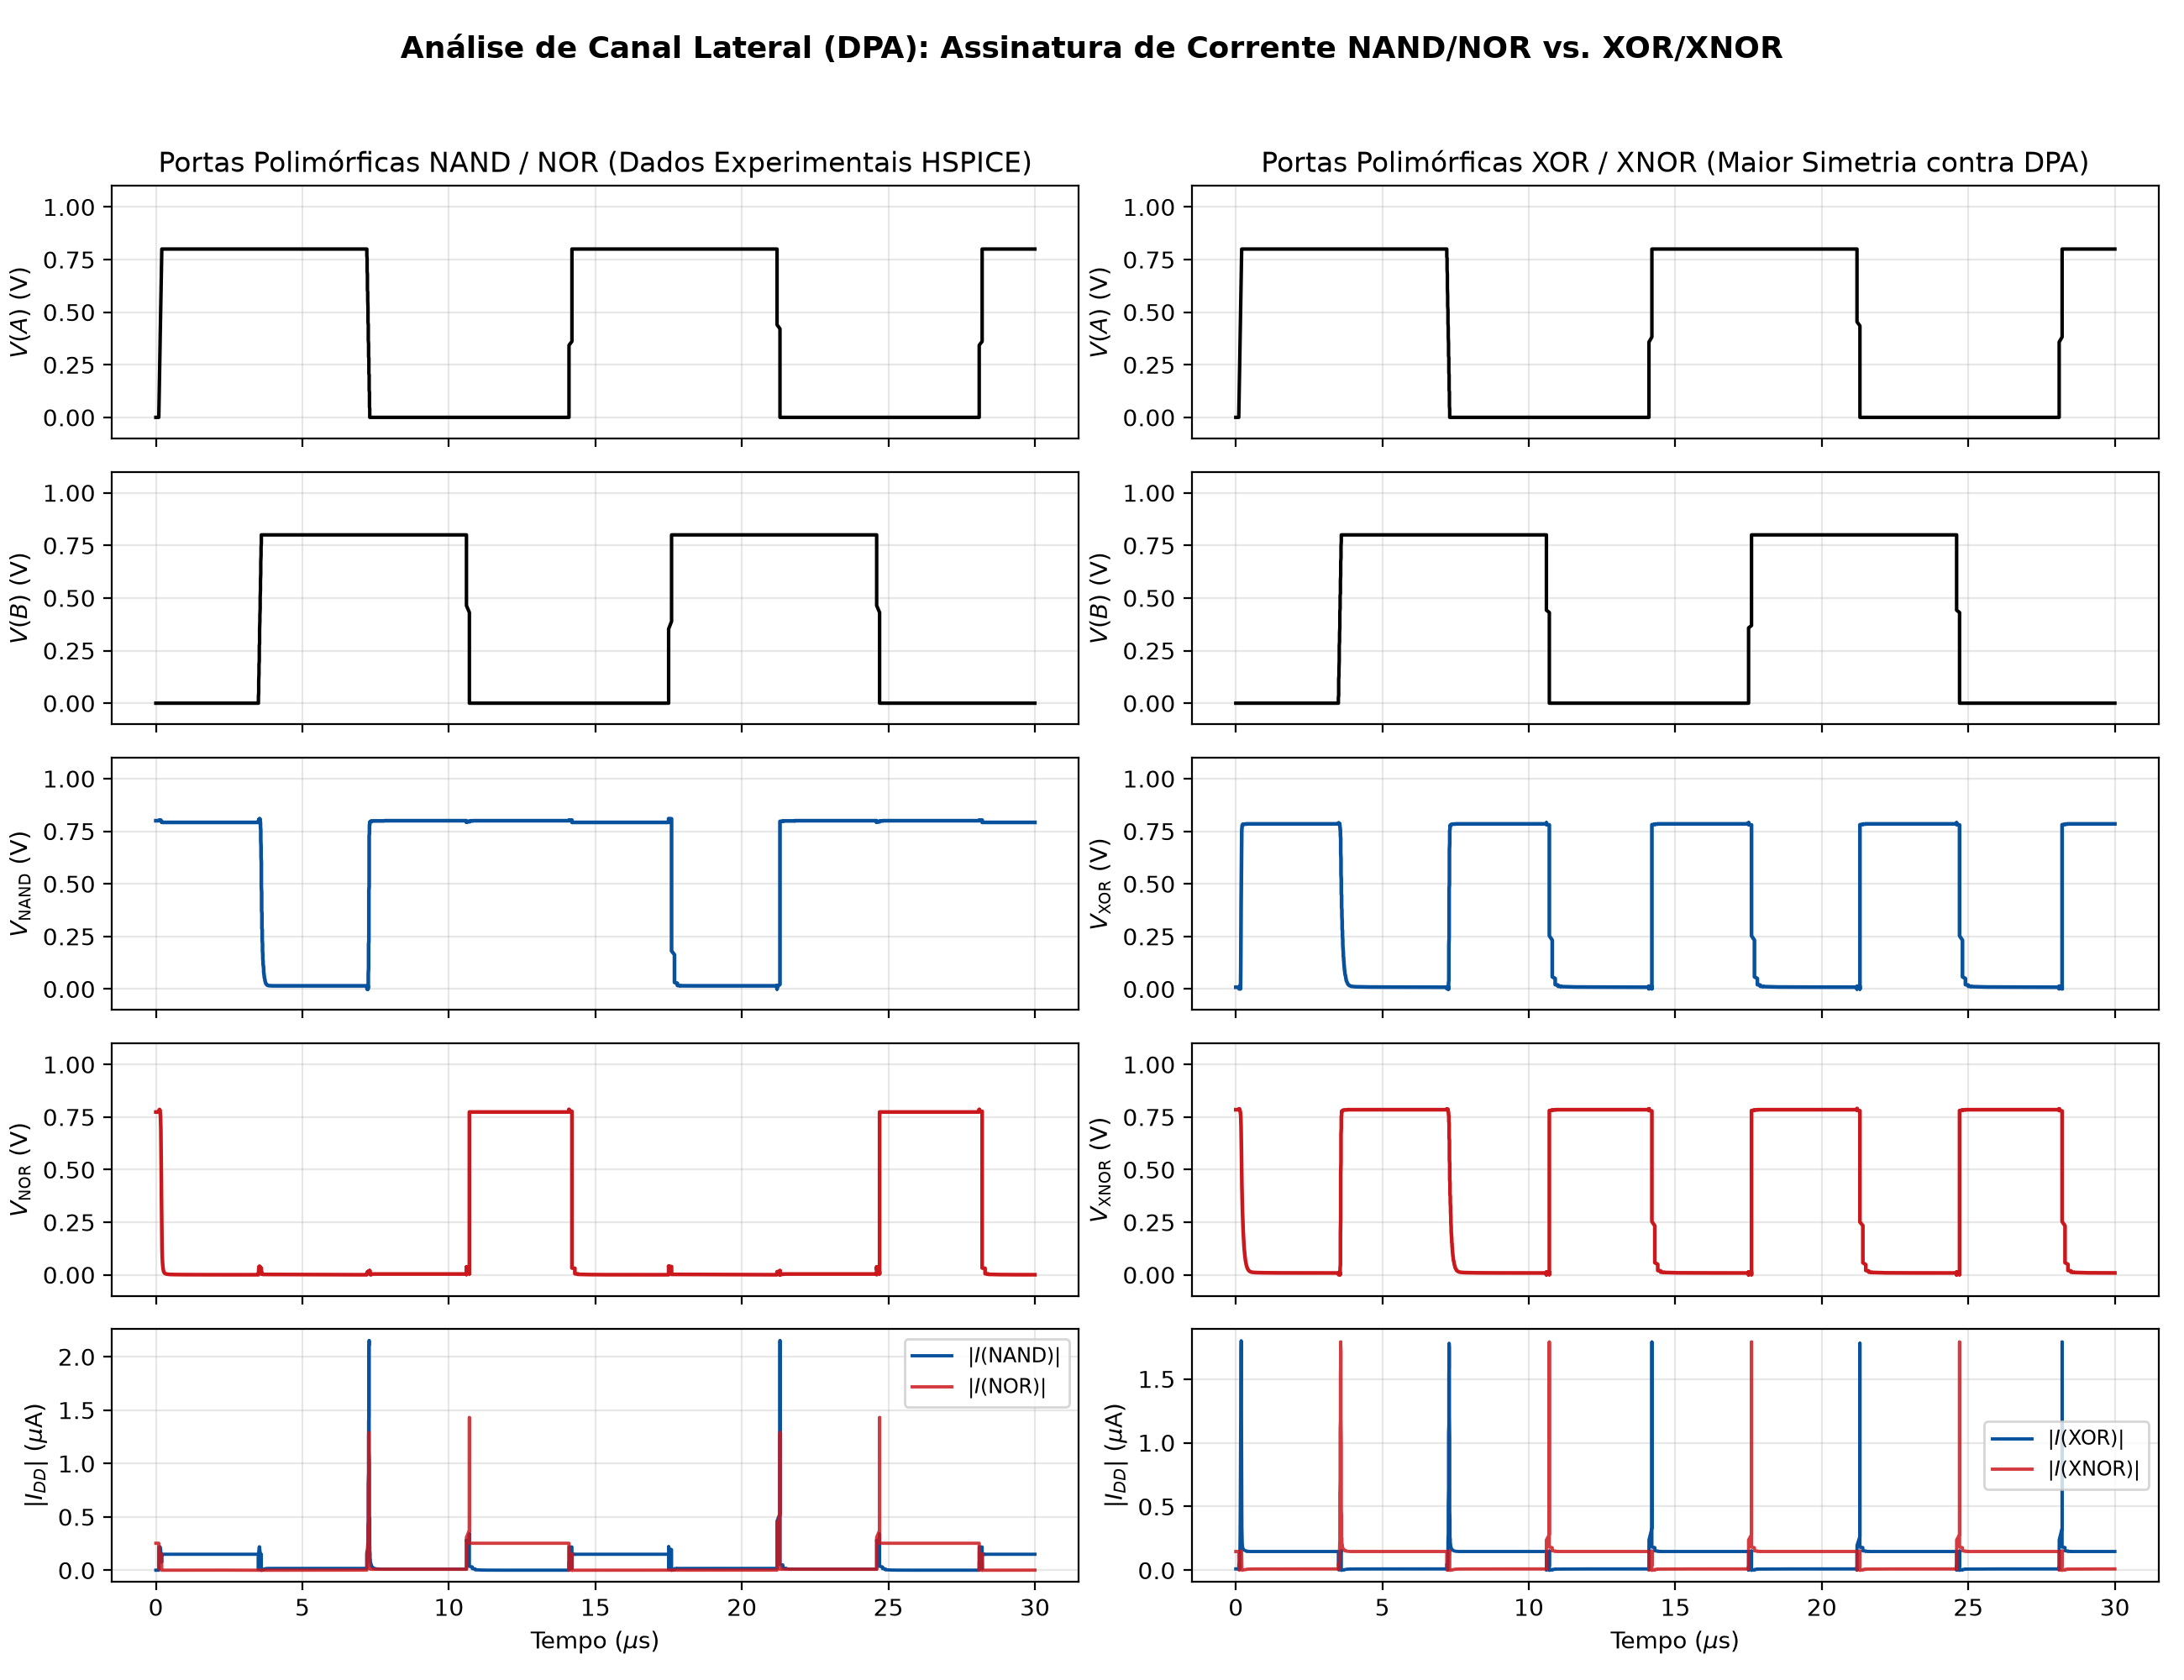
\includegraphics[width=0.92\textwidth]{m03_dpa_assinatura_corrente.png}
\caption{Side-channel DPA current signature comparison ($|I_{DD}|$) between \texttt{NAND}/\texttt{NOR} (left) and \texttt{XOR}/\texttt{XNOR} (right).}
\label{fig:m03_dpa}
\end{figure}

Across all 250 Monte Carlo samples (Figure~\ref{fig:m03_mc3d}), even under severe supply rail fluctuations ($V_{DD} \in [0.47,\ 1.15]\ \text{V}$), all four gates maintained $100.0\%$ logic accuracy with clean separation between \texttt{'0'} and \texttt{'1'} around $0.40\ \text{V}$. Cross-validation on the $5 \times 5$ \texttt{ngspice-47} grid (\texttt{ngspice\_supply\_sweep.csv}, Figure~\ref{fig:m03_hist_ret}) confirmed static margins $(V_{00} - V_{11})$ between $0.531\ \text{V}$ and $1.012\ \text{V}$ whenever $V_{DD} \ge 0.725\ \text{V}$ or $V_{SS} \ge -0.05\ \text{V}$, narrowing to $0.153\ \text{V}$ only at the worst-case corner ($V_{DD}=0.65\ \text{V},\ V_{SS}=-0.10\ \text{V}$, where $V_{00}=0.060\ \text{V}$ and $V_{11}=-0.093\ \text{V}$). For floating-node retention (\texttt{bblc1}), following excitation pulses at $40$ and $80\ \mu\text{s}$, the node stabilized at distinct plateaus of $0.65\ \text{V}$ ($100\ \text{ns}$), $0.30\ \text{V}$ ($250\ \text{ns}$), and $0.20\ \text{V}$ ($500\ \text{ns}$) through $111\ \mu\text{s}$.

\begin{figure}[htbp]
\centering
\begin{subfigure}{\textwidth}
  \centering
  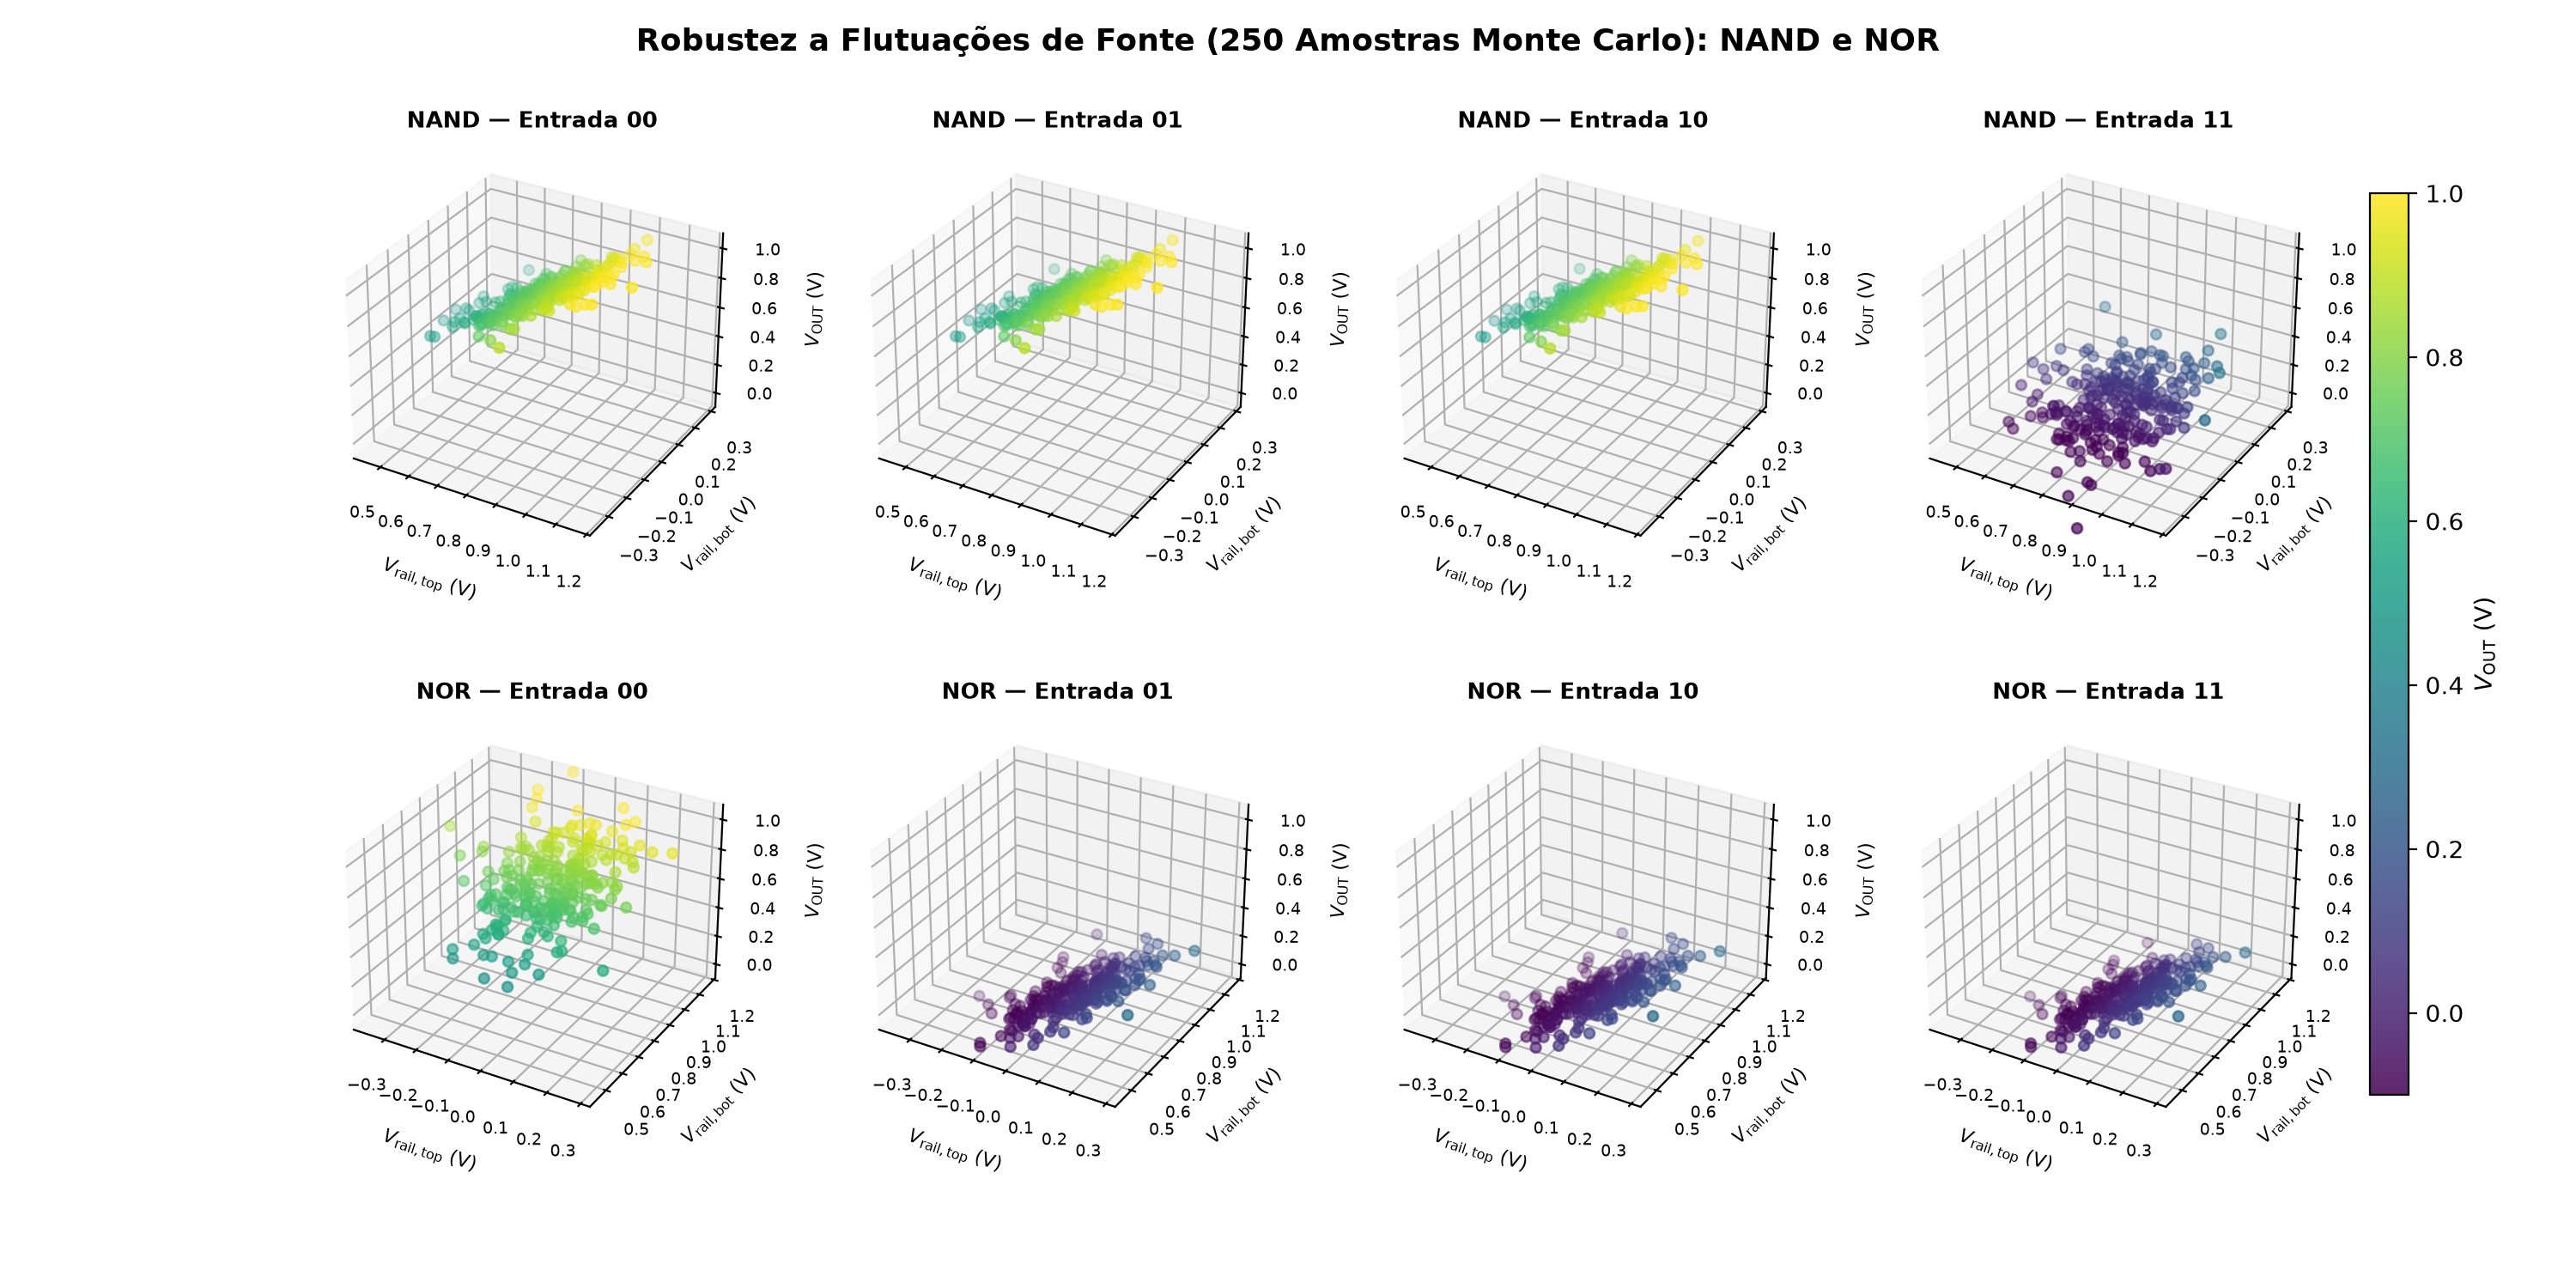
\includegraphics[width=0.95\textwidth]{m03_robustez_3d_nand_nor.png}
  \caption{\texttt{NAND} and \texttt{NOR} gates.}
  \label{fig:m03_3d_nn}
\end{subfigure}
\par\medskip
\begin{subfigure}{\textwidth}
  \centering
  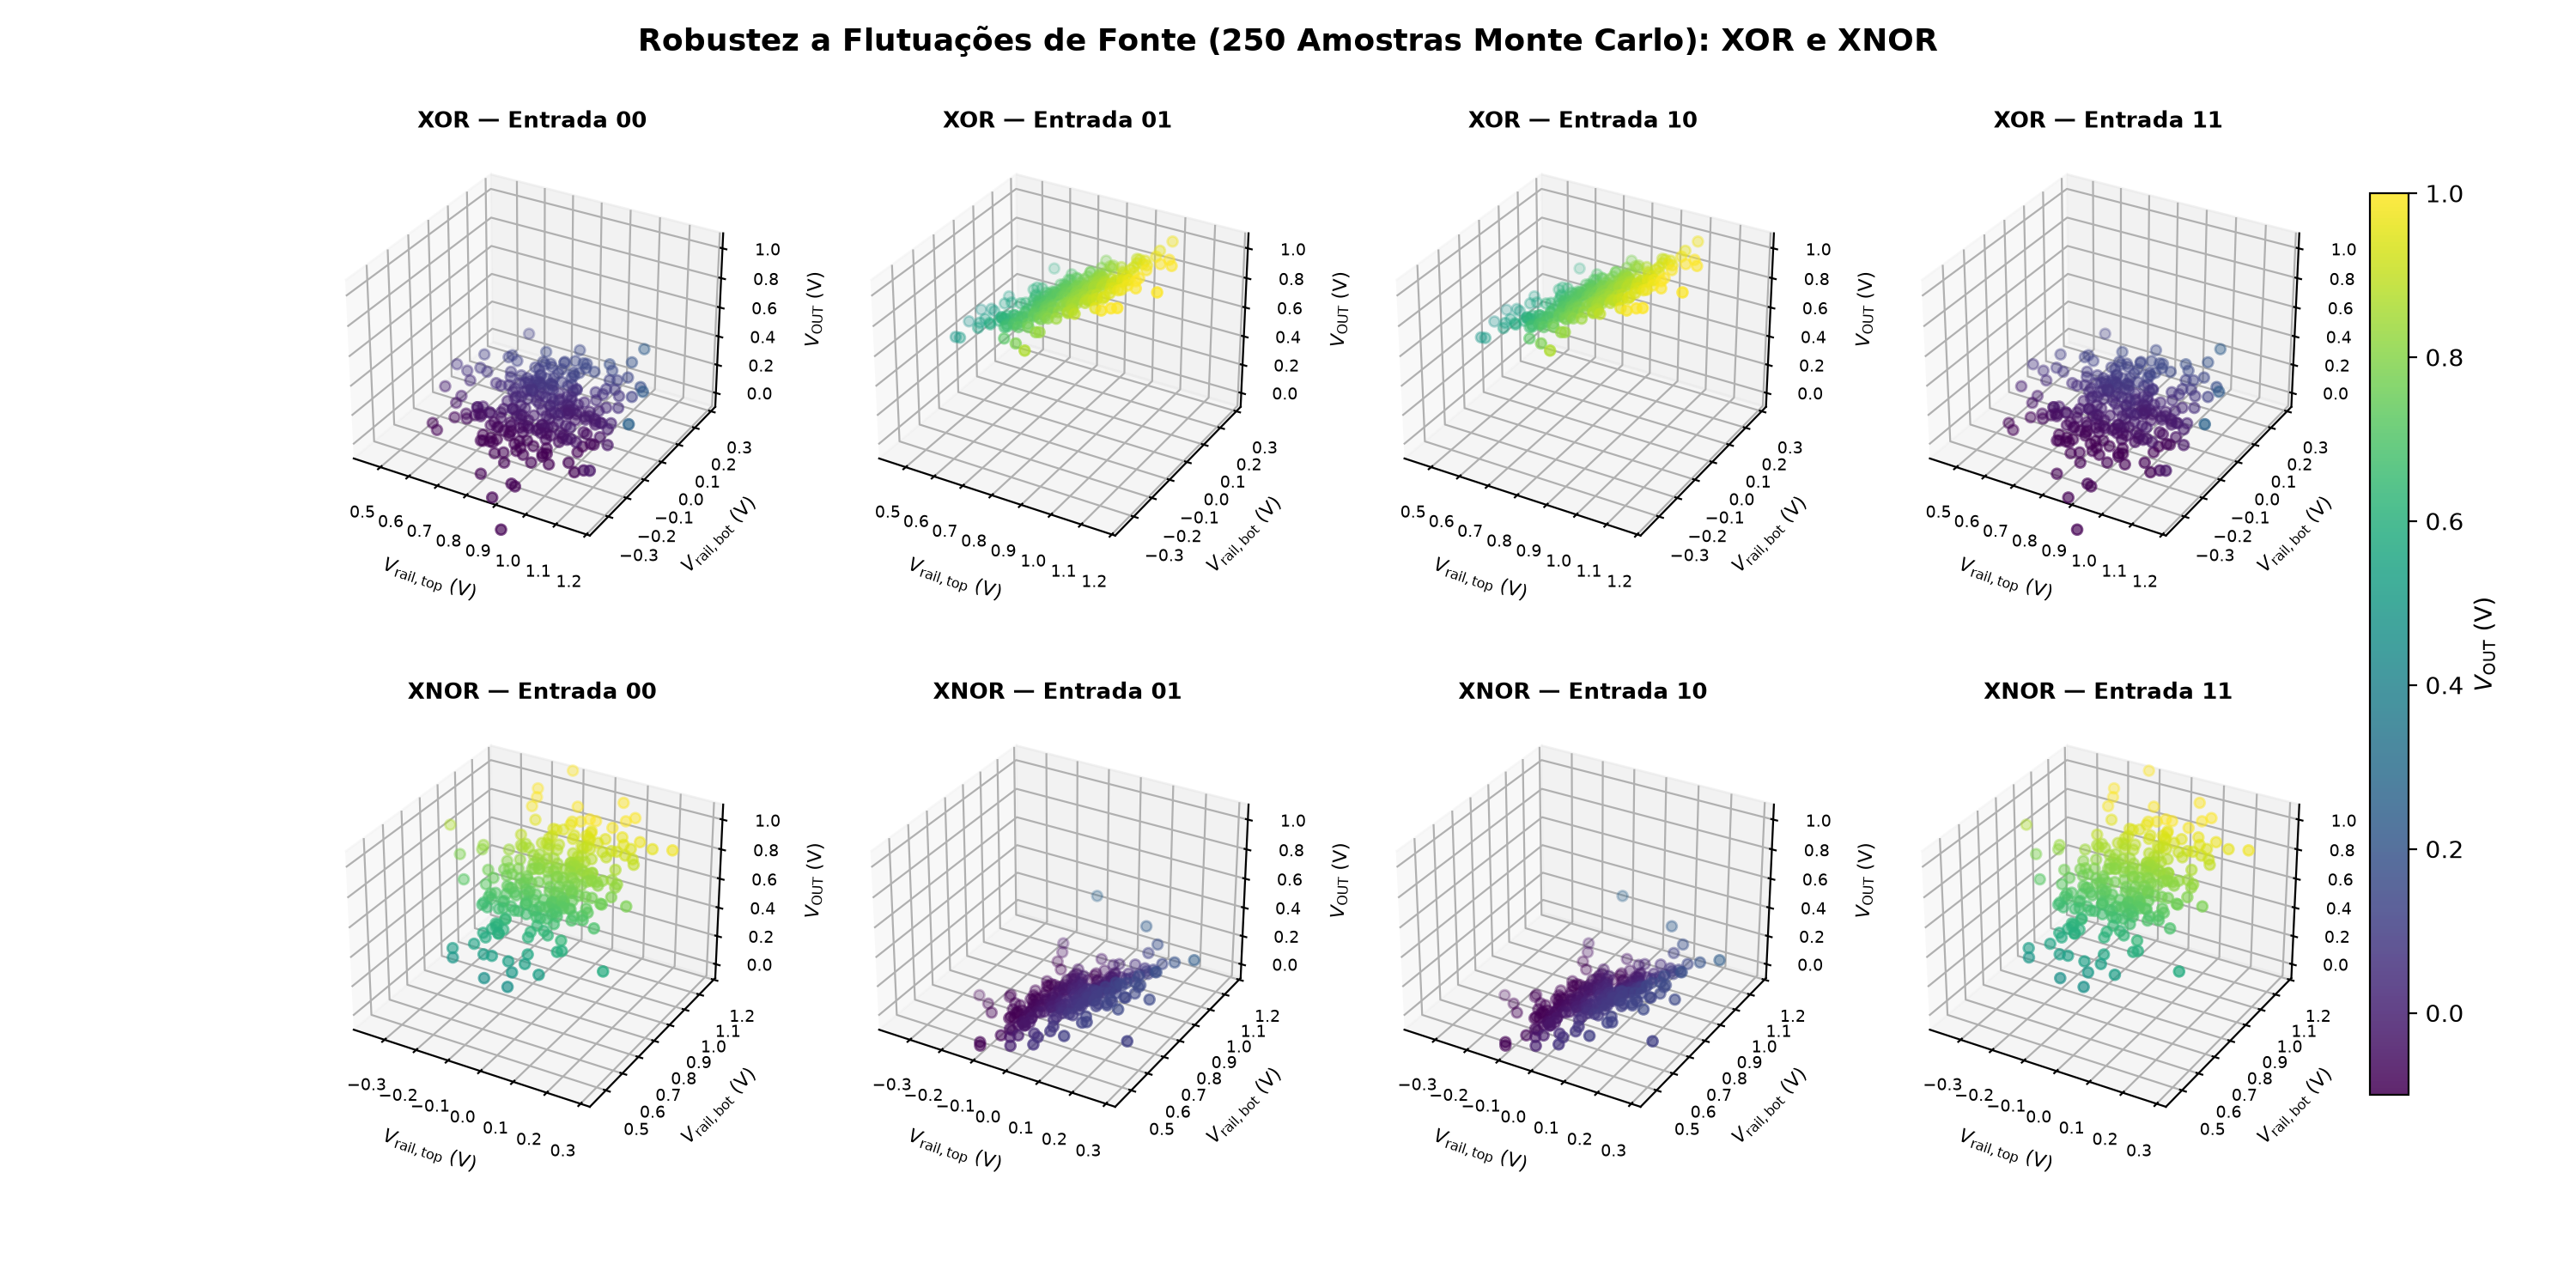
\includegraphics[width=0.95\textwidth]{m03_robustez_3d_xor_xnor.png}
  \caption{\texttt{XOR} and \texttt{XNOR} gates.}
  \label{fig:m03_3d_xx}
\end{subfigure}
\caption{3D robustness surfaces ($V_{\mathrm{rail,top}} \times V_{\mathrm{rail,bot}} \times V_{\mathrm{OUT}}$) across 250 Monte Carlo samples per input vector.}
\label{fig:m03_mc3d}
\end{figure}

\begin{figure}[htbp]
\centering
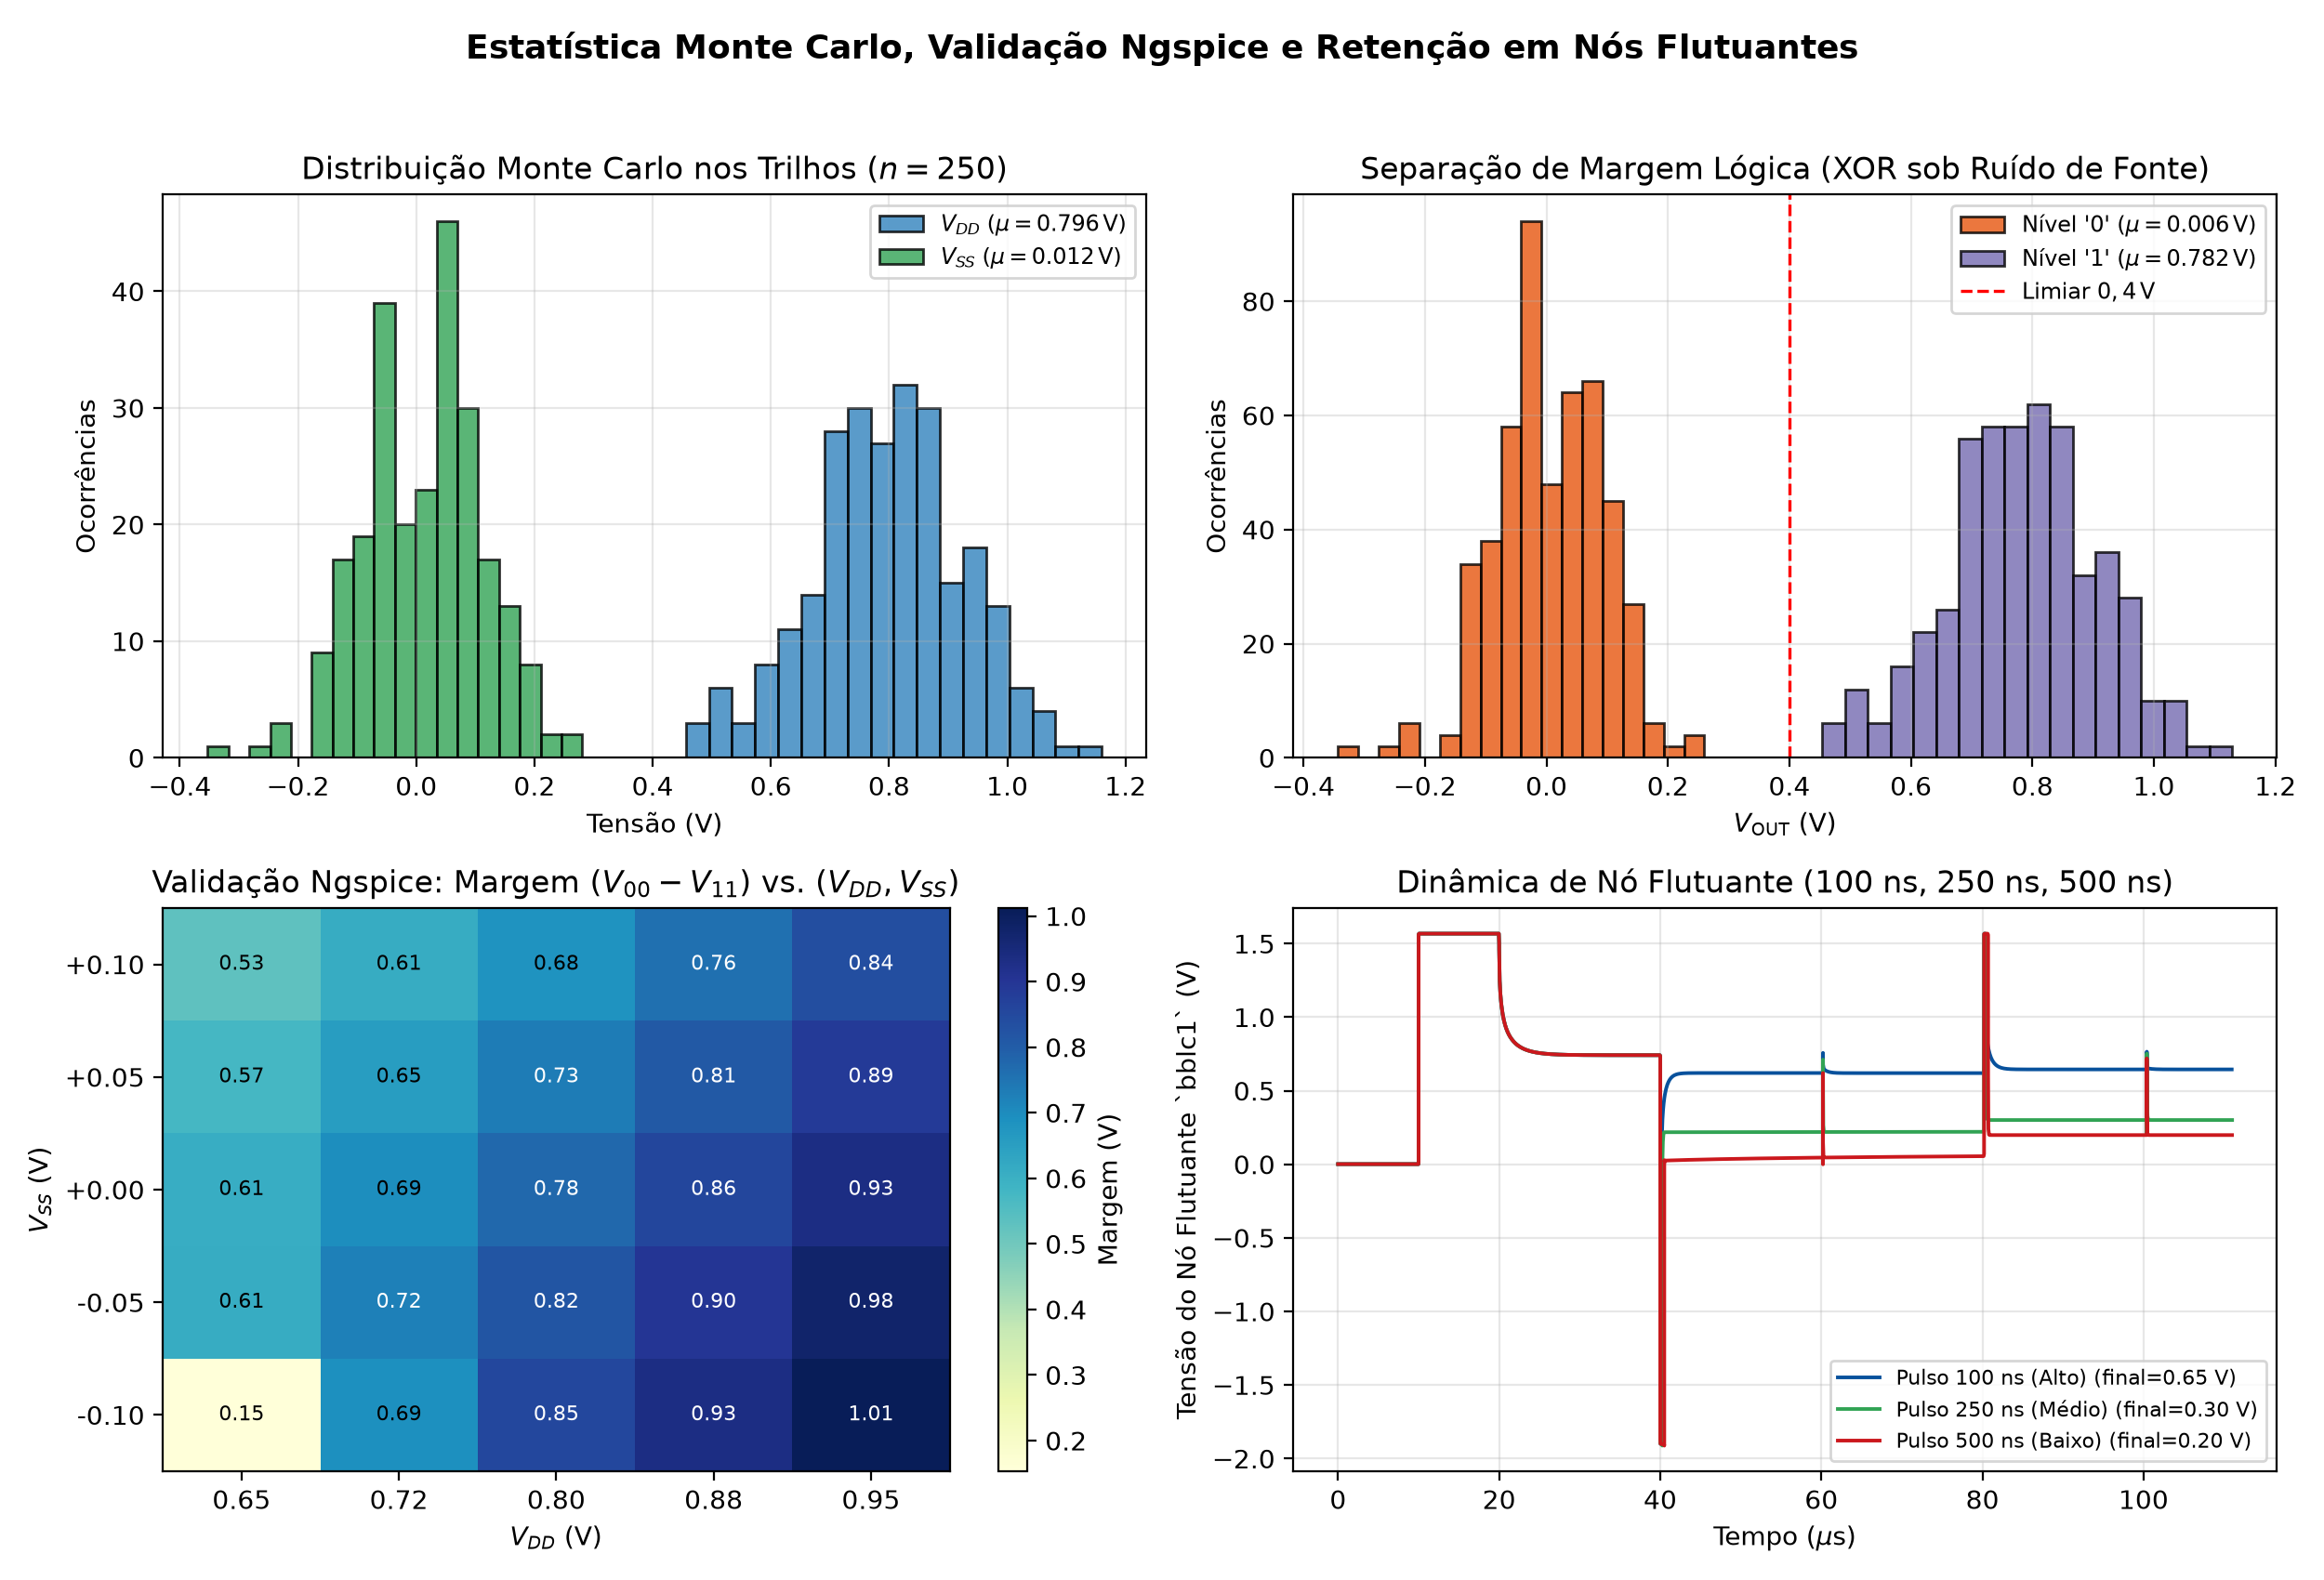
\includegraphics[width=0.92\textwidth]{m03_histogramas_e_retencao.png}
\caption{Monte Carlo rail distribution (top left), \texttt{XOR} logic-level separation (top right), \texttt{ngspice-47} $V_{DD}\times V_{SS}$ margin map (bottom left), and floating-node \texttt{bblc1} retention up to $111\ \mu\text{s}$ (bottom right).}
\label{fig:m03_hist_ret}
\end{figure}

\subsection{6T SRAM Cell with Retention Locking (Mechanism B)}\label{sec:res_sram}

The 6T SRAM cell passed all eleven transient and static acceptance criteria for Mechanism B, as summarized in Table~\ref{tab:sram_results}. During the $30\ \text{ns}$ transient simulation (Figure~\ref{fig:m04_tran}), under $\text{Key} = 0$, the bit \texttt{'1'} written in $0\text{--}6\ \text{ns}$ is stably retained after wordline de-assertion with $V(q) = 0.9768\ \text{V}$ and $V(qb) = 0.0020\ \text{V}$ at $t=12\ \text{ns}$ ($\Delta V_{\mathrm{Key0}} = 0.9747\ \text{V} > 0.80\ \text{V}$). Once $\text{Key}$ switches to $1$ ($t = 15\ \text{ns}$), while keeping $V_{DD} = 1.0\ \text{V}$ and $V_{SS} = 0.0\ \text{V}$ constant, simultaneous inversion of pull-up (\textit{p-FET} $\to$ \textit{n-FET}) and pull-down (\textit{n-FET} $\to$ \textit{p-FET}) devices triggers immediate collapse of the stored bit ($\Delta V_{\mathrm{Collapse1}} = 0.0841\ \text{V} < 0.15\ \text{V}$ at $18\ \text{ns}$). In Phase~4 ($20\text{--}30\ \text{ns}$), even after forcing the opposite bit while $\mathrm{WL}$ is asserted, the cell collapses again as soon as $\mathrm{WL}$ closes ($\Delta V_{\mathrm{Key1}} = 0.0762\ \text{V}$ at $28\ \text{ns}$).

\begin{table}[htbp]
\centering
\caption{Transient ($30\ \text{ns}$) and static noise margin (SNM) metrics of the 6T SRAM cell (\texttt{metricas\_sram\_6t.csv}).}
\label{tab:sram_results}
\footnotesize
\begin{tabular}{l c c c}
\toprule
\textbf{Extracted Metric} & \textbf{Simulated Value} & \textbf{Acceptance Criterion} & \textbf{Status} \\
\midrule
$V(q)_{\mathrm{Hold}}$ ($\text{Key}=0,\ t=12\ \text{ns}$)   & $0.9768\ \text{V}$ & $> 0.80\ \text{V}$ & Passed \\
$V(qb)_{\mathrm{Hold}}$ ($\text{Key}=0,\ t=12\ \text{ns}$)  & $0.0020\ \text{V}$ & $< 0.20\ \text{V}$ & Passed \\
$\Delta V_{\mathrm{Key0}}$ ($t=12\ \text{ns}$)              & $0.9747\ \text{V}$ & $> 0.80\ \text{V}$ & Passed \\
$\Delta V_{\mathrm{Collapse1}}$ ($t=18\ \text{ns}$)         & $0.0841\ \text{V}$ & $< 0.15\ \text{V}$ & Passed \\
$\Delta V_{\mathrm{Key1}}$ ($t=28\ \text{ns}$)              & $0.0762\ \text{V}$ & $< 0.15\ \text{V}$ & Passed \\
$\mathrm{SNM}_{\mathrm{Hold}}$ ($\text{Key}=0,\ \mathrm{WL}=0\ \text{V}$)           & $167.12\ \text{mV}$ & $> 150\ \text{mV}$ & Passed \\
$\mathrm{SNM}_{\mathrm{Read,Unassisted}}$ ($\text{Key}=0,\ \mathrm{WL}=1.0\ \text{V}$) & $0.00\ \text{mV}$ & $0\ \text{mV}$ (\textit{Read Disturb}) & Diagnosed \\
$\mathrm{SNM}_{\mathrm{Read,Assist}}$ ($\text{Key}=0,\ \mathrm{WL}=0.30\ \text{V}$) & $66.23\ \text{mV}$ & $> 50\ \text{mV}$ & Passed \\
$\mathrm{SNM}_{\mathrm{Hold}}$ ($\text{Key}=1,\ \mathrm{WL}=0\ \text{V}$)           & $0.00\ \text{mV}$ & $= 0\ \text{mV}$ & Passed \\
$\mathrm{SNM}_{\mathrm{Read,Assist}}$ ($\text{Key}=1,\ \mathrm{WL}=0.30\ \text{V}$) & $0.00\ \text{mV}$ & $= 0\ \text{mV}$ & Passed \\
$\mathrm{SNM}_{\mathrm{Read,Unassisted}}$ ($\text{Key}=1,\ \mathrm{WL}=1.0\ \text{V}$) & $0.00\ \text{mV}$ & $= 0\ \text{mV}$ & Passed \\
\bottomrule
\end{tabular}
\end{table}

\begin{figure}[htbp]
\centering
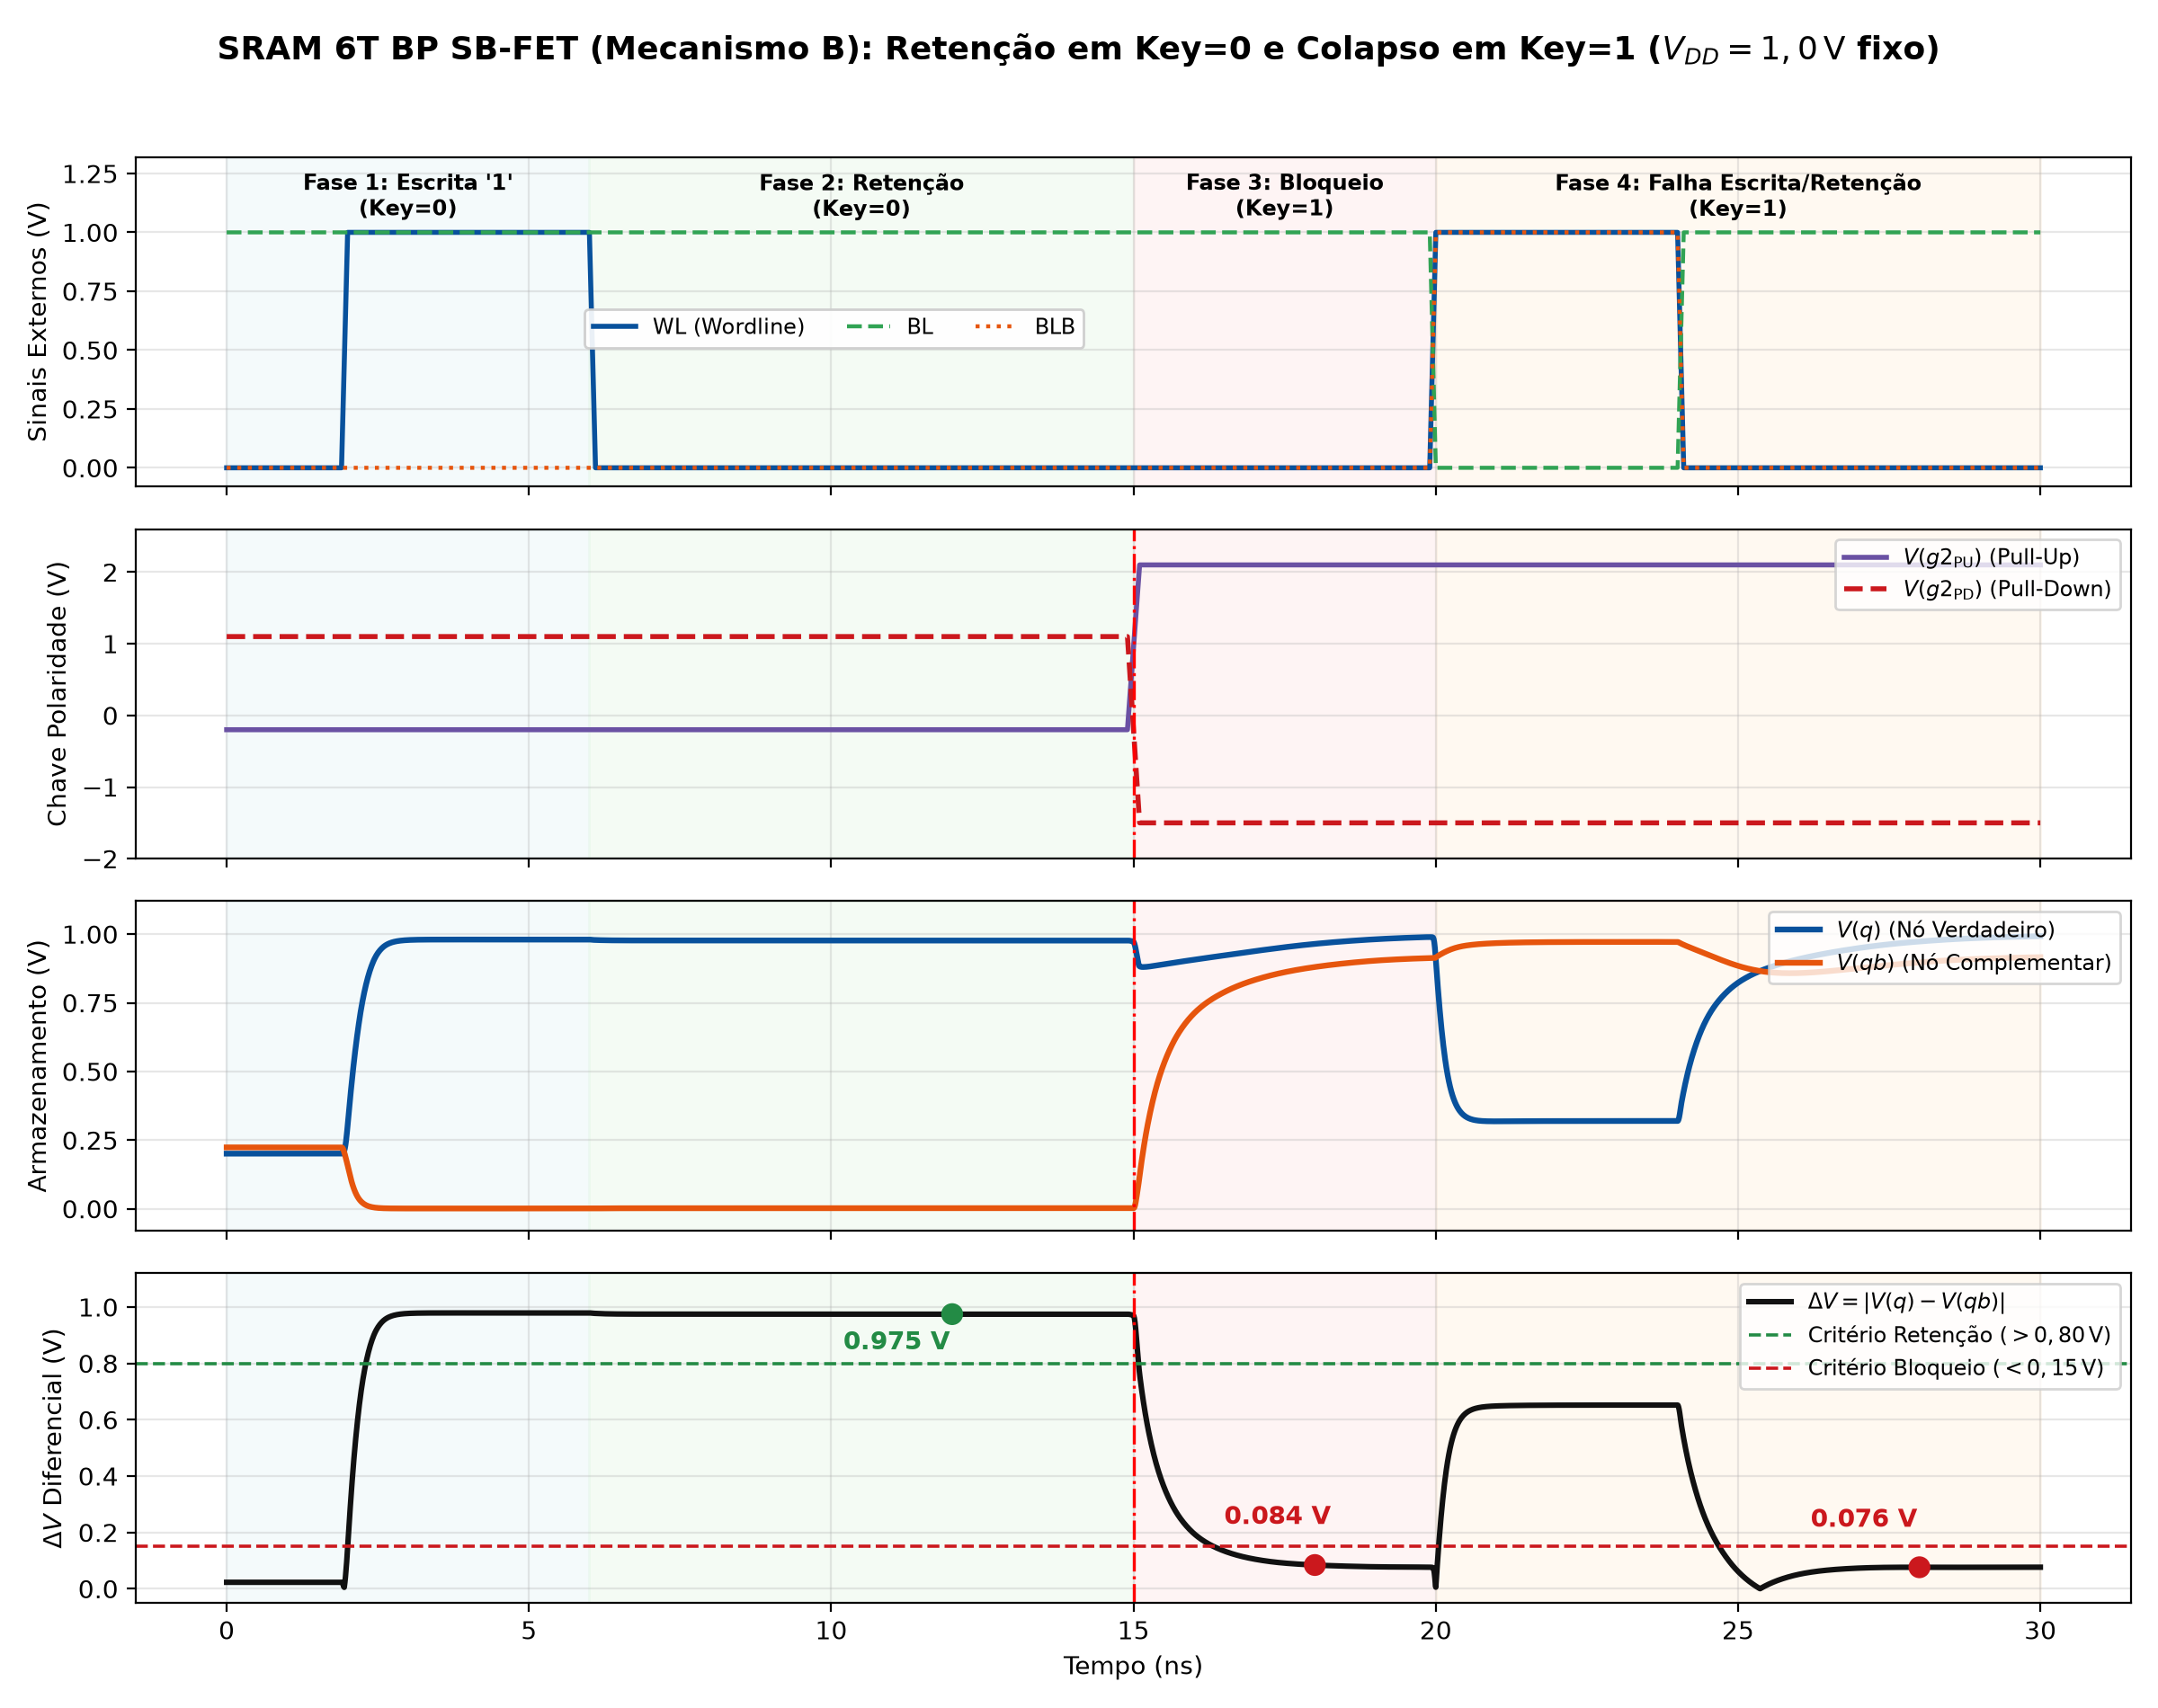
\includegraphics[width=0.92\textwidth]{m04_sram_transiente_30ns.png}
\caption{Four-phase $30\ \text{ns}$ transient simulation of the 6T SRAM cell: write and stable retention under $\text{Key}=0$ ($0\text{--}15\ \text{ns}$) followed by self-destruction and rewrite failure under $\text{Key}=1$ ($15\text{--}30\ \text{ns}$).}
\label{fig:m04_tran}
\end{figure}

\begin{figure}[htbp]
\centering
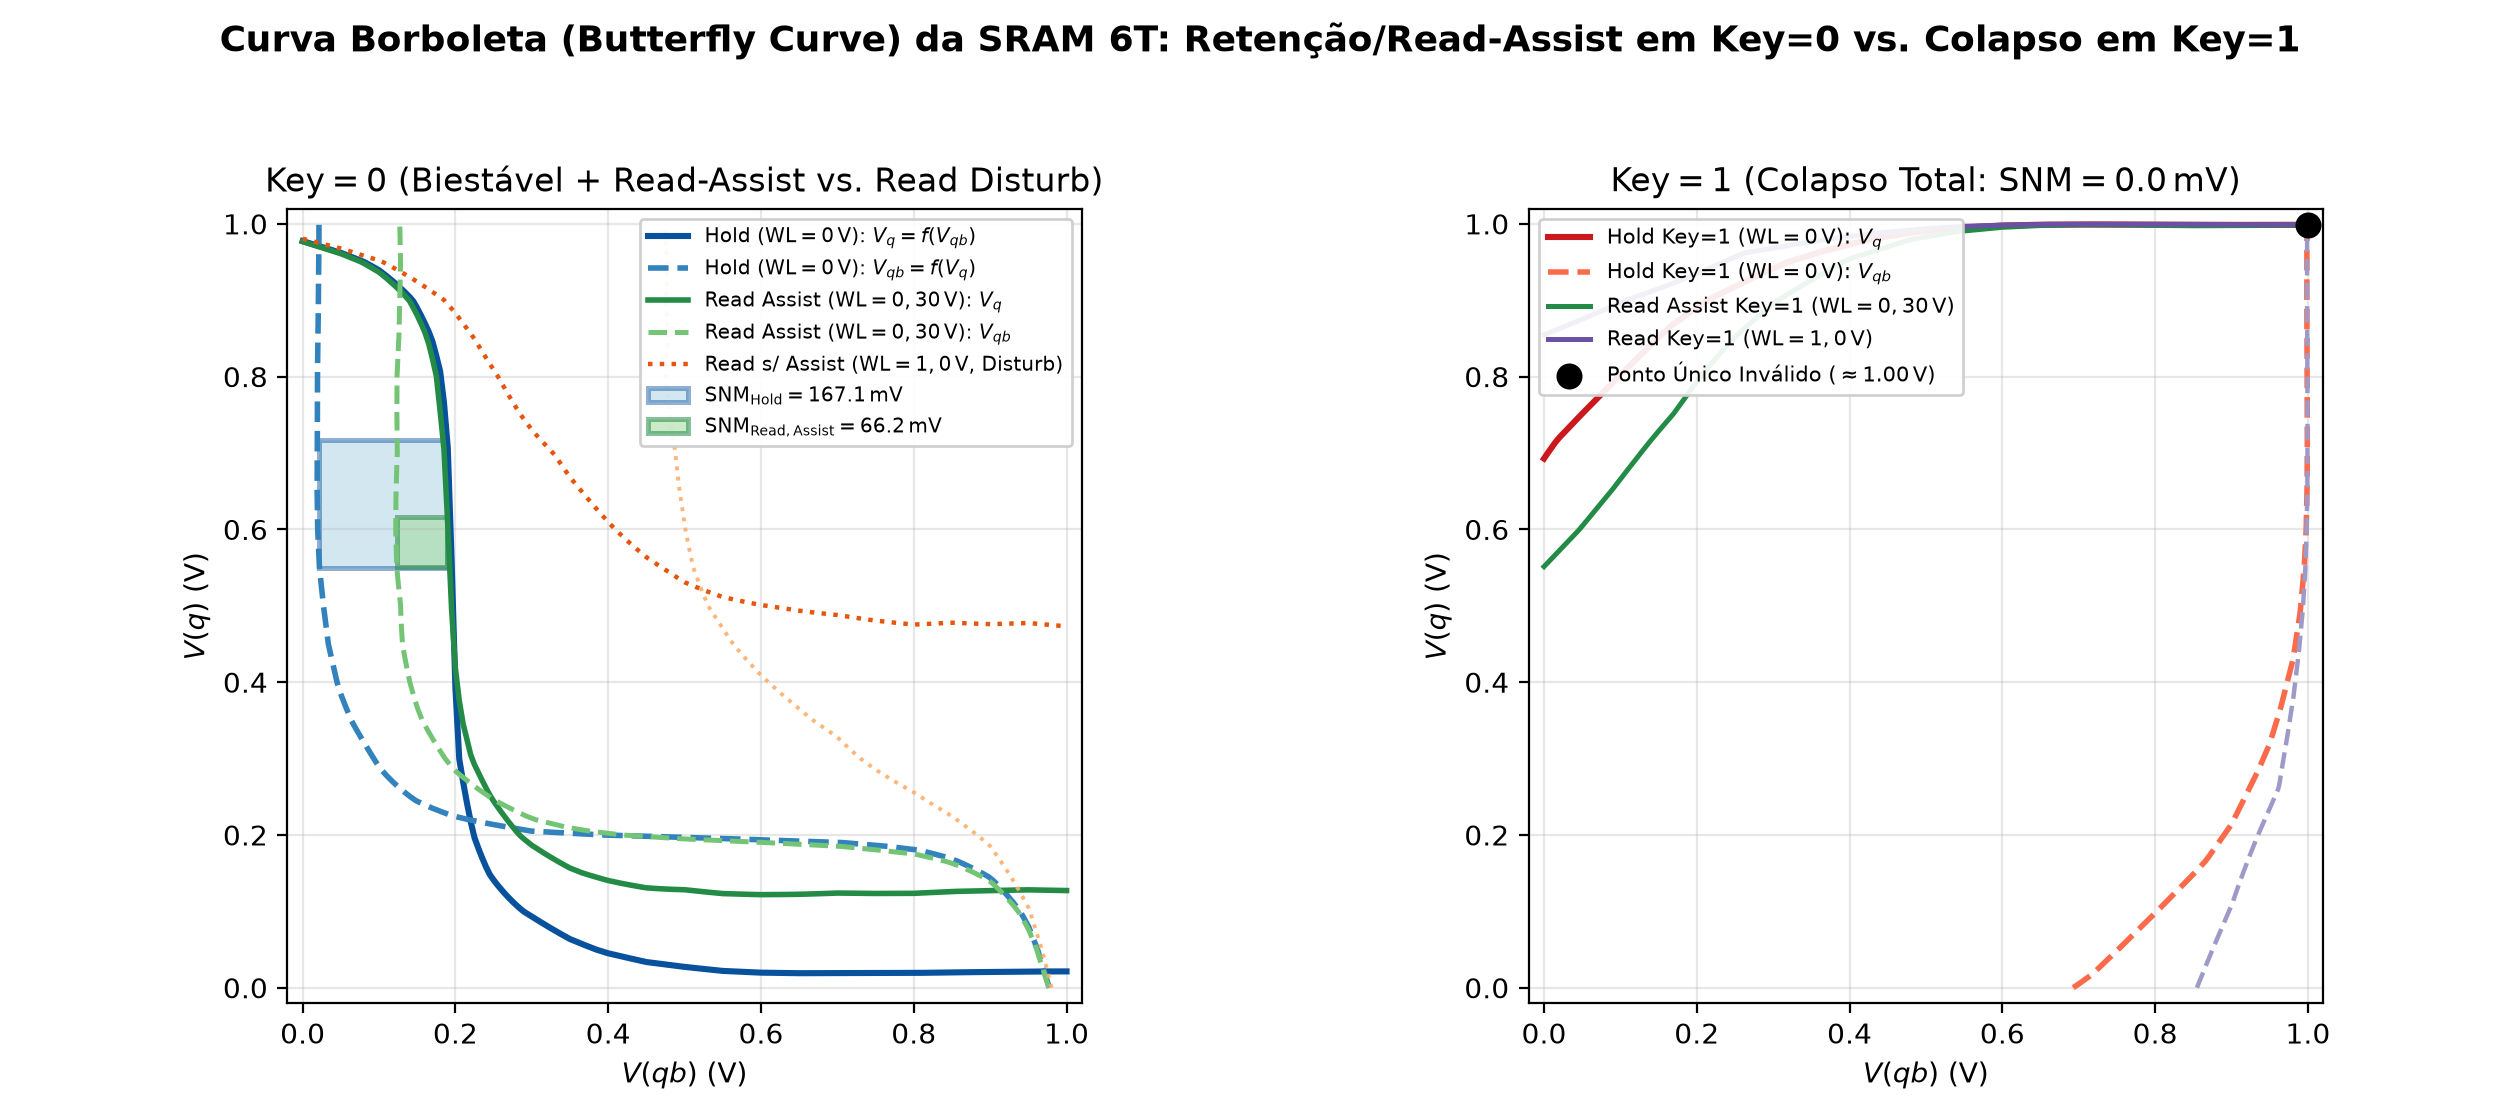
\includegraphics[width=0.92\textwidth]{m04_sram_curva_borboleta_snm.png}
\caption{6T SRAM butterfly curves and maximum inscribed SNM squares for $\text{Key}=0$ (Hold, Read-Assist, and Unassisted Read showing \textit{Read Disturb}) and $\text{Key}=1$ (total monostable collapse).}
\label{fig:m04_snm}
\end{figure}

Two important physical findings emerged from the butterfly-curve analysis (Figure~\ref{fig:m04_snm}). First, simulations with the 4D \texttt{v2} model revealed that the initially proposed $V_{g2,\mathrm{PU}} = -0.5\ \text{V}$ ($V_{g2,s} = -1.5\ \text{V}$) bias reduces \textit{p-FET} current from $1.79$ to $0.37\ \mu\text{A}$ (at $V_{gp}=-1.0\ \text{V}$) due to flat-band shift, lowering $\mathrm{SNM}_{\mathrm{Hold}}$ to $49.4\ \text{mV}$; tuning to $V_{g2,\mathrm{PU}} = -0.2\ \text{V}$ ($V_{g2,s} = -1.2\ \text{V}$) fully restored symmetry without altering device widths $W$, recovering $\mathrm{SNM}_{\mathrm{Hold}} = 167.12\ \text{mV}$. Second, unassisted reading ($\mathrm{WL}=1.0\ \text{V}$) exhibited destructive \textit{Read Disturb} ($\mathrm{SNM}=0.00\ \text{mV}$), which was mitigated via \textit{Wordline Underdrive Read-Assist} at $\mathrm{WL}=0.30\ \text{V}$, restoring $\mathrm{SNM}_{\mathrm{Read,Assist}} = 66.23\ \text{mV}$ while all $\text{Key}=1$ conditions remained locked at $\mathrm{SNM}=0.00\ \text{mV}$.

\subsection{Cryptographic Polymorphic Full Adder (28 Transistors)}\label{sec:res_fa}

In the 28-transistor polymorphic Full Adder (Module~\texttt{05}), the authorized key $K_1 K_0 = 00$ achieved $100.00\%$ truth-table accuracy across all eight minterms ($000 \to 111$, Figure~\ref{fig:m05_wave}), maintaining over $94\%$ swing on \texttt{Sum} ($1.5\ \text{V}$ domain: \texttt{'0'} $\le 0.0012\ \text{V}$, \texttt{'1'} $\ge 1.4129\ \text{V}$) and over $92\%$ swing on \texttt{Cout} ($0.8\ \text{V}$ domain: \texttt{'0'} $\le 0.0124\ \text{V}$, \texttt{'1'} $\ge 0.7526\ \text{V}$) across three cascaded logic levels.

\begin{table}[htbp]
\centering
\caption{Functional corruption and Hamming Distance (HD) per cryptographic key $(K_1, K_0)$ in the 28T Full Adder.}
\label{tab:fa_hamming}
\resizebox{\textwidth}{!}{%
\begin{tabular}{c l c c c c c c}
\toprule
\textbf{Key} $K_1K_0$ & \textbf{Configuration} (\texttt{XXOR1} + \texttt{Cout}) & \texttt{Sum} \textbf{Errors} & \textbf{HD} \texttt{Sum} & \texttt{Cout} \textbf{Errors} & \textbf{HD} \texttt{Cout} & \textbf{Total HD} (/16) & \textbf{Accuracy} \\
\midrule
\texttt{00} (Correct) & \texttt{XOR} + \texttt{NAND}  & $0/8$ & $0.0\%$   & $0/8$ & $0.0\%$  & $0\ (0.00\%)$   & $100.00\%$ \\
\texttt{01} (Wrong)   & \texttt{XNOR} + \texttt{NAND} & $8/8$ & $100.0\%$ & $3/8$ & $37.5\%$ & $11\ (68.75\%)$ & $31.25\%$  \\
\texttt{10} (Wrong)   & \texttt{XOR} + \texttt{NOR}   & $0/8$ & $0.0\%$   & $3/8$ & $37.5\%$ & $3\ (18.75\%)$  & $81.25\%$  \\
\texttt{11} (Wrong)   & \texttt{XNOR} + \texttt{NOR}  & $8/8$ & $100.0\%$ & $0/8$ & $0.0\%$  & $8\ (50.00\%)$  & $50.00\%$  \\
\bottomrule
\end{tabular}}
\end{table}

As shown in Table~\ref{tab:fa_hamming} and Figure~\ref{fig:m05_hd}, every incorrect key corrupts the arithmetic output without requiring extra dedicated locking transistors. At $K_1K_0 = 01$, inversion of $P \to \overline{P}$ propagates errors to both \texttt{Sum} ($100.0\%$) and \texttt{Cout} ($37.5\%$), yielding $\mathrm{HD}_{\mathrm{Total}} = 68.75\%$. At $K_1K_0 = 11$, De Morgan duality emerges: switching both \texttt{XXOR1} to \texttt{XNOR} ($\overline{P}$) and \texttt{XG1}--\texttt{XG3} to \texttt{NOR} produces $\overline{\overline{A+B} + \overline{\overline{P}+C_{\mathrm{in}}}} = (A+B)\cdot(\overline{P}+C_{\mathrm{in}}) = A\cdot B + C_{\mathrm{in}}\cdot(A\oplus B)$, restoring \texttt{Cout} while \texttt{Sum} remains $100.0\%$ inverted ($\mathrm{HD}_{\mathrm{Total}} = 50.00\%$).

\begin{figure}[htbp]
\centering
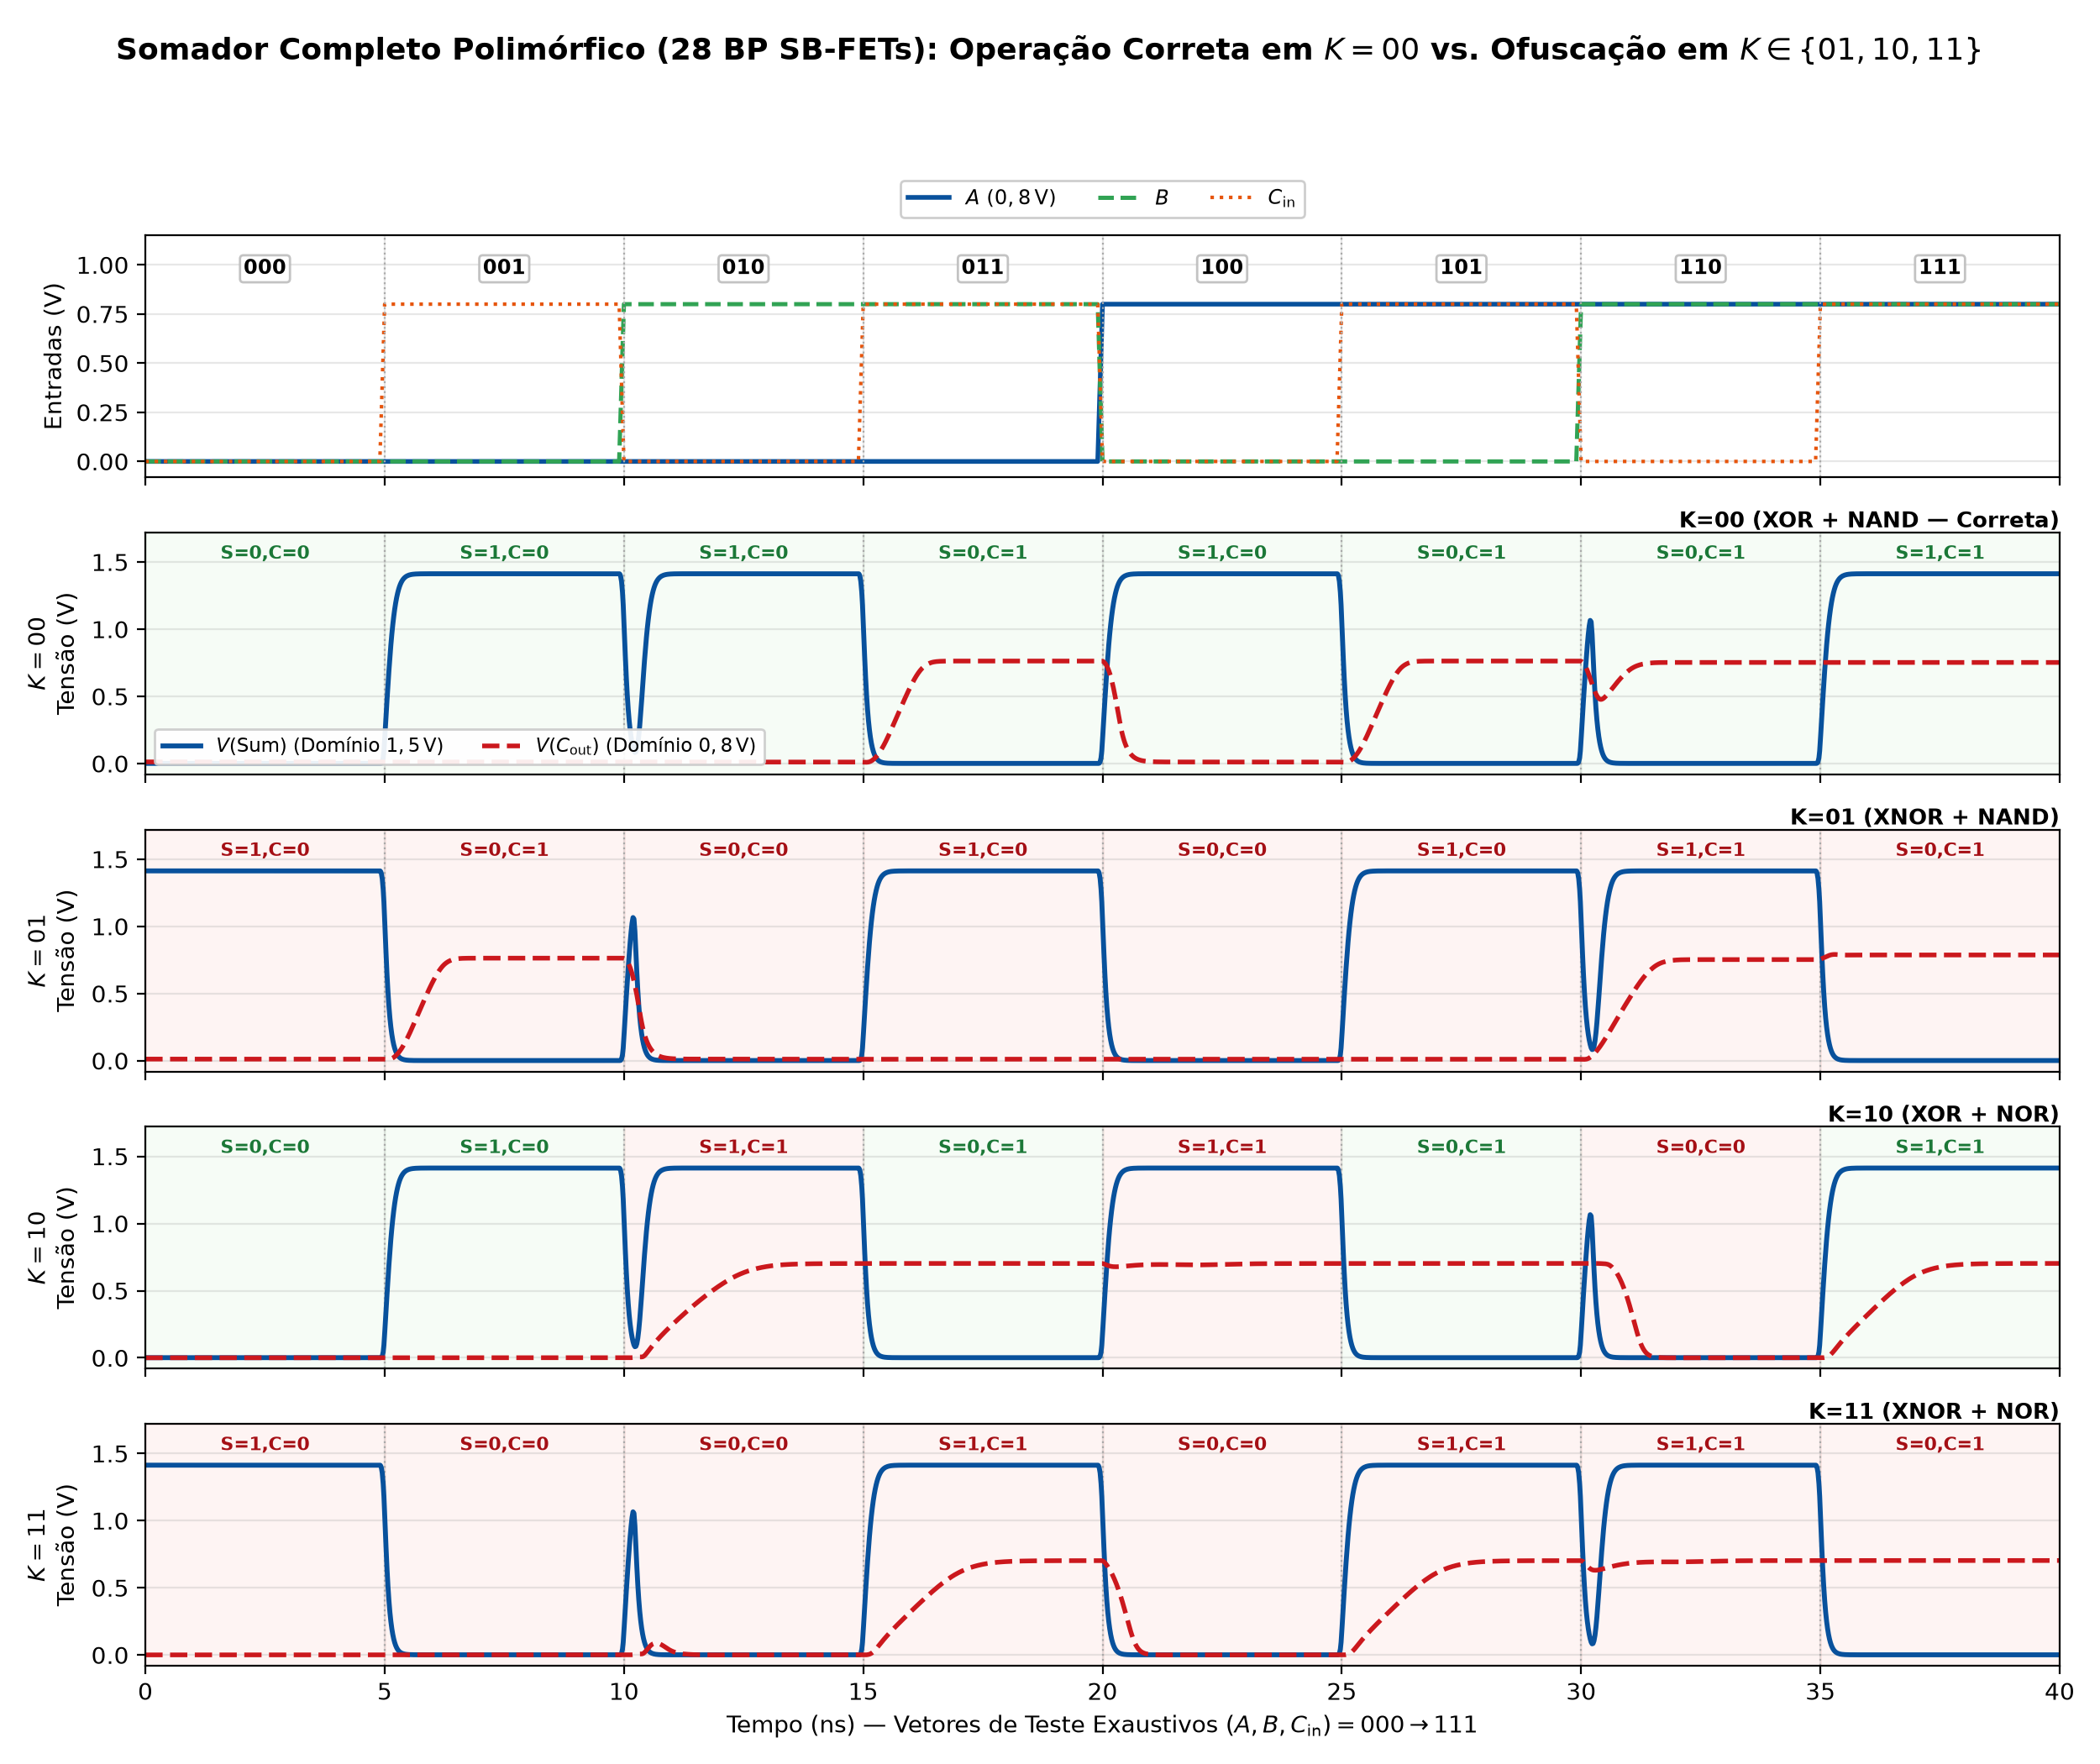
\includegraphics[width=0.92\textwidth]{m05_full_adder_waveforms.png}
\caption{Exhaustive transient waveforms ($40\ \text{ns}$, minterms \texttt{000} to \texttt{111}) of the 28-transistor polymorphic Full Adder across all four keys $K_1K_0$.}
\label{fig:m05_wave}
\end{figure}

\begin{figure}[htbp]
\centering
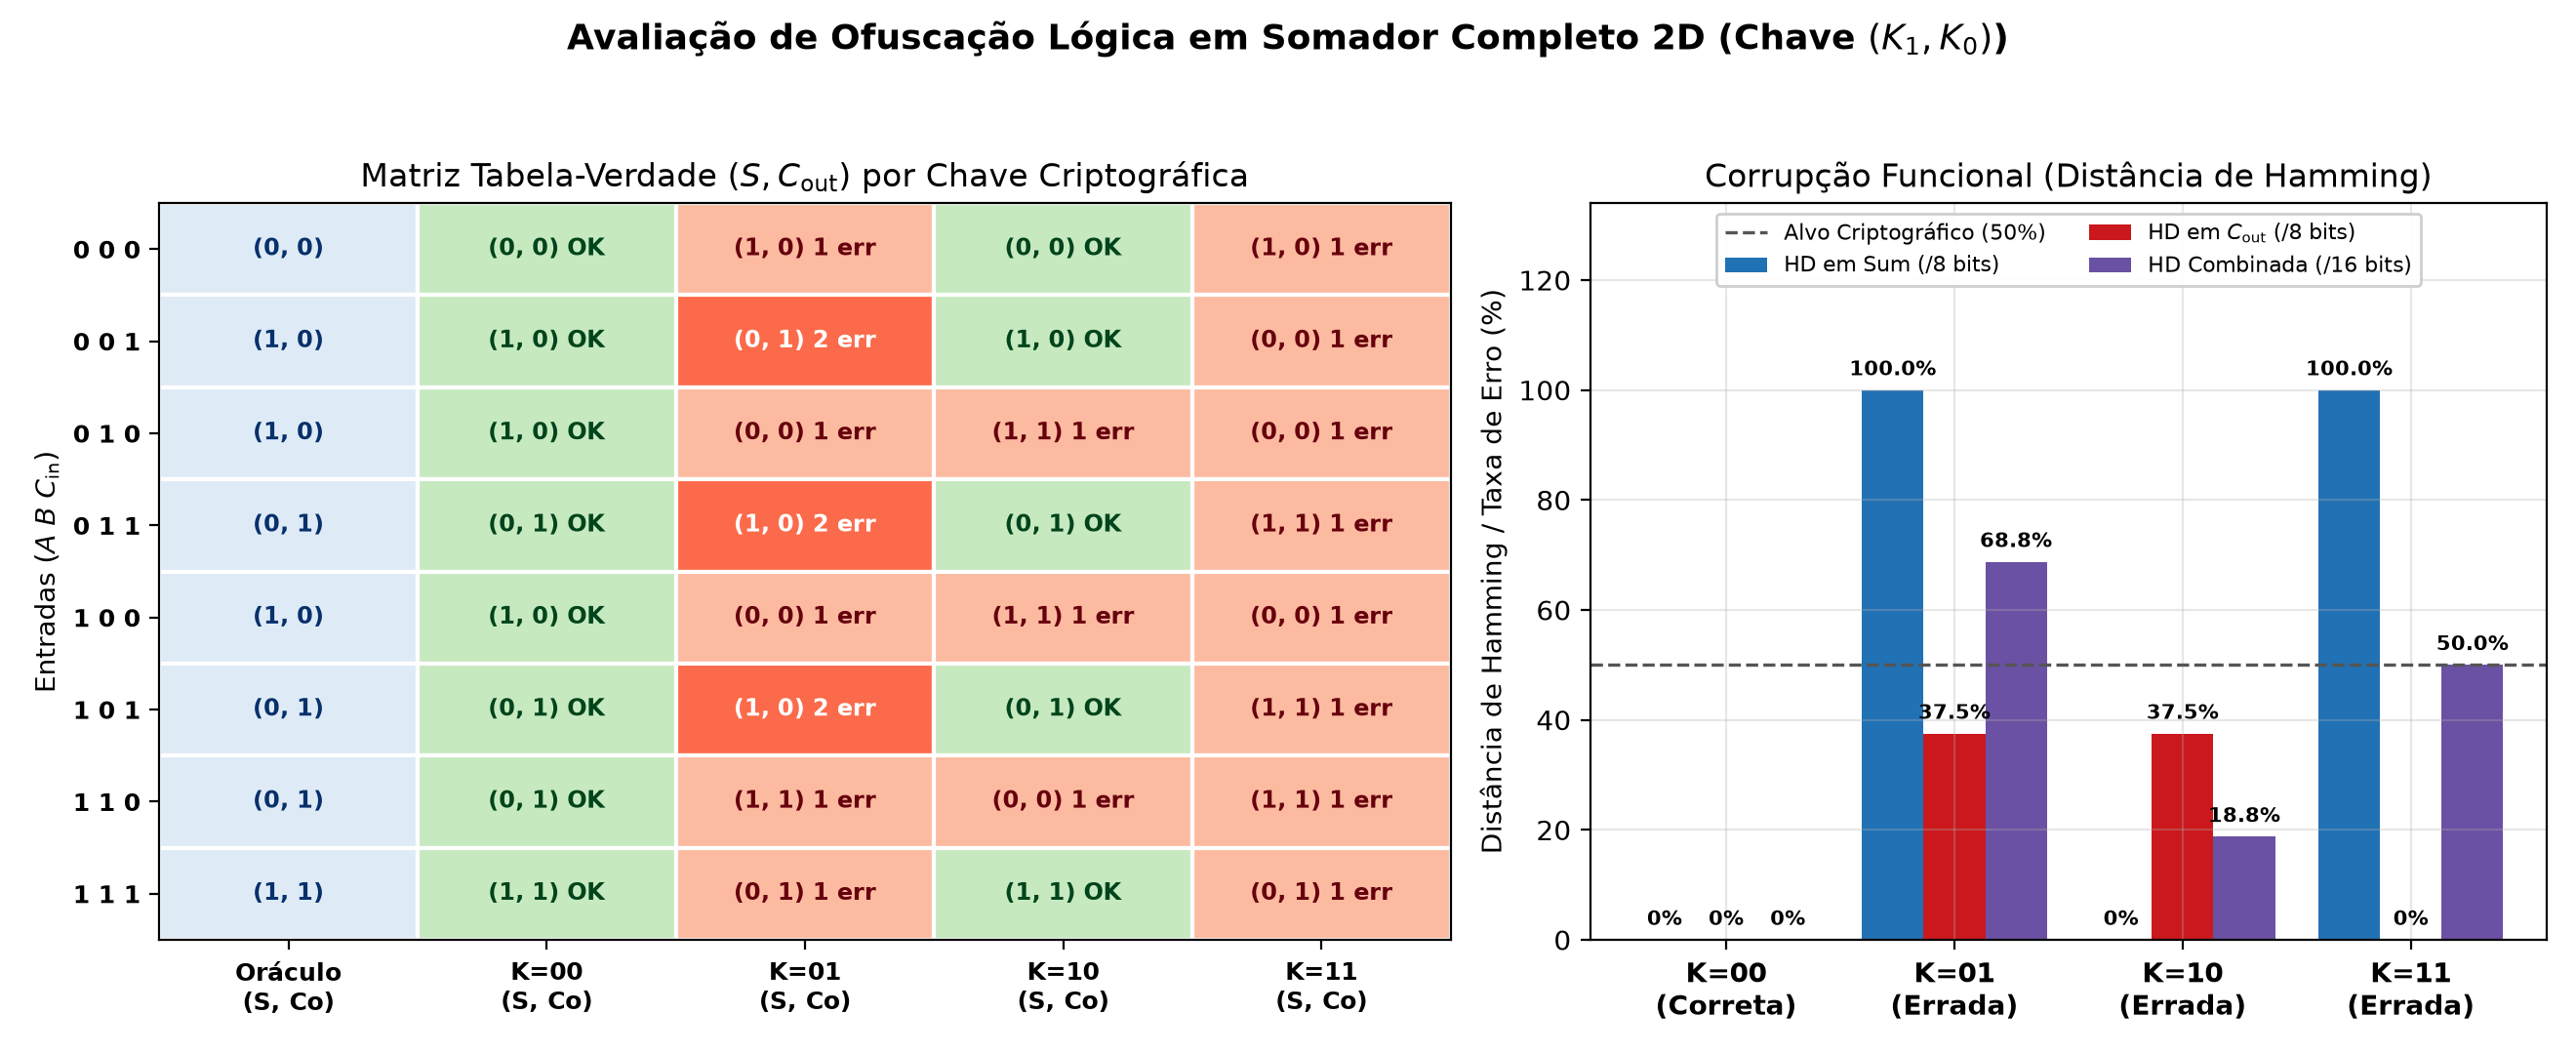
\includegraphics[width=0.92\textwidth]{m05_matriz_tabelas_verdade_hamming.png}
\caption{Truth-table matrix and Hamming Distance (HD) of the polymorphic Full Adder for keys \texttt{00}, \texttt{01}, \texttt{10}, and \texttt{11}.}
\label{fig:m05_hd}
\end{figure}

\subsection{Operating Boundaries under Non-Standard Voltages}\label{sec:res_boundary}

Sweeping 292 points inside the experimentally measured LUT domain (Module~\texttt{06}) confirmed that shifting supply, input, and polarity voltages can trigger all three hypothesized outcomes: preservation of the target function (\texttt{CORRETA}), transmutation into another digital Boolean function (\texttt{OUTRA\_FUNCAO}), or collapse into intermediate analog states (\texttt{INDEFINIDO\_ANALOGICO}), as summarized in Table~\ref{tab:boundary_summary}.

\begin{table}[htbp]
\centering
\caption{Classification of the 292 operating points simulated under non-standard voltages within the LUT domain.}
\label{tab:boundary_summary}
\resizebox{\textwidth}{!}{%
\begin{tabular}{l c c c c l}
\toprule
\textbf{Sub-experiment} & \textbf{Points} & \texttt{CORRETA} & \texttt{OUTRA\_FUNCAO} & \texttt{INDEFINIDO} & \textbf{Observed Equivalent Functions} \\
\midrule
\texttt{NAND}/\texttt{NOR} ($V_{DD}\times$ Pol.) & $70$  & $29$ & $35$ & $6$  & \texttt{NAND} ($13$), \texttt{NOR} ($17$), \texttt{CONST\_0} ($34$), \texttt{X} ($6$) \\
\texttt{NAND}/\texttt{NOR} ($V_{g2,n}\times V_{g2,p}$) & $72$  & $60$ & $0$  & $12$ & \texttt{NAND} ($27$), \texttt{NOR} ($33$), \texttt{X} ($12$) \\
\texttt{XOR}/\texttt{XNOR} ($V_{DD}\times V_{\mathrm{in}}$) & $100$ & $44$ & $46$ & $10$ & \texttt{XOR} ($22$), \texttt{XNOR} ($22$), \texttt{CONST\_0} ($38$), \texttt{CONST\_1} ($8$), \texttt{X} ($10$) \\
\texttt{XOR}/\texttt{XNOR} ($V_{g,\mathrm{top}}=0\ \text{V}$) & $50$  & $44$ & $6$  & $0$  & \texttt{XOR} ($22$), \texttt{XNOR} ($22$), \texttt{CONST\_1} ($6$) \\
\bottomrule
\end{tabular}}
\end{table}

In the \texttt{NAND}/\texttt{NOR} family (Figures~\ref{fig:m06_nn_vdd} and \ref{fig:m06_nn_asym}), a critical event of \textbf{spontaneous \texttt{NAND} $\to$ \texttt{NOR} conversion without key switching} was identified: at $V_{DD} = 0.65\ \text{V}$ under moderate sub-polarization ($+0.4/-1.1\ \text{V}$), the gate configured as \texttt{NAND} ($\text{Key}=0$) produced the bit pattern \texttt{[1000]} ($V_{00}=0.5412\ \text{V}$, $V_{01}=0.1073\ \text{V}$, $V_{10}=0.1410\ \text{V}$, $V_{11}=0.0206\ \text{V}$), matching the truth table of its dual \texttt{NOR} function. Physically, for inputs \texttt{01} and \texttt{10}, a single weakened \textit{p-FET} cannot overcome leakage through the $+0.4\ \text{V}$-biased \textit{n-FET} series path, and pull-up succeeds only when both parallel \textit{p-FETs} conduct (\texttt{00}). For $V_{DD} \le 0.50\ \text{V}$, $34$ of $70$ points collapsed to \texttt{CONST\_0} (\texttt{0000}). In the $V_{DD}=0.80\ \text{V}$ asymmetry grid, $60$ of $72$ points functioned properly while $12$ entered analog undefined states (\texttt{[1X10]}, \texttt{[10X0]}, \texttt{[111X]}, \texttt{[X000]}), highlighting a non-monotonic degradation along $V(g2,s)_p = -1.50\ \text{V}$ in \texttt{NAND} (caused by the $\Delta V_{fb} \approx -0.25\ \text{V}$ shift, collapsing $V_{01}$ to $0.163\text{--}0.496\ \text{V}$ in four of six \textit{n-FET} columns), whereas $V(g2,s)_p \in \{-1.35,\ -1.20\}\ \text{V}$ achieved $100\%$ accuracy.

In the \texttt{XOR}/\texttt{XNOR} family (Figure~\ref{fig:m06_xor_map}), $150$ points were evaluated ($88$ correct, $52$ classified as \texttt{OUTRA\_\allowbreak FUNCAO}, and $10$ in \texttt{INDEFINIDO\_\allowbreak ANALOGICO}), exposing opposite stuck-at regimes: for $V_{DD} \in [0.60,\ 0.80]\ \text{V}$, $38$ cases collapsed to \texttt{CONST\_0} (\texttt{0000}) due to insufficient \textit{p-FET} overdrive; conversely, at high $V_{DD}$ ($1.20\text{--}1.50\ \text{V}$) and low $V_{\mathrm{in}}$ ($0.40\text{--}0.60\ \text{V}$), $14$ cases latched to \texttt{CONST\_1} (\texttt{1111}, $V_{\mathrm{out}} \ge 1.4154\ \text{V}$ at $1.50\ \text{V}$) with elevated static current ($0.536\text{--}1.222\ \mu\text{A}$). Along the intermediate boundary ($V_{DD} = 1.00\ \text{V}$), nominal bias ($+0.8/-1.5\ \text{V}$) became undefined for $V_{\mathrm{in}} \ge 0.80\ \text{V}$, whereas sub-polarization ($+0.2/-0.9\ \text{V}$) restored correct operation with $86.4\%\text{--}88.4\%$ normalized margin.

\begin{figure}[htbp]
\centering
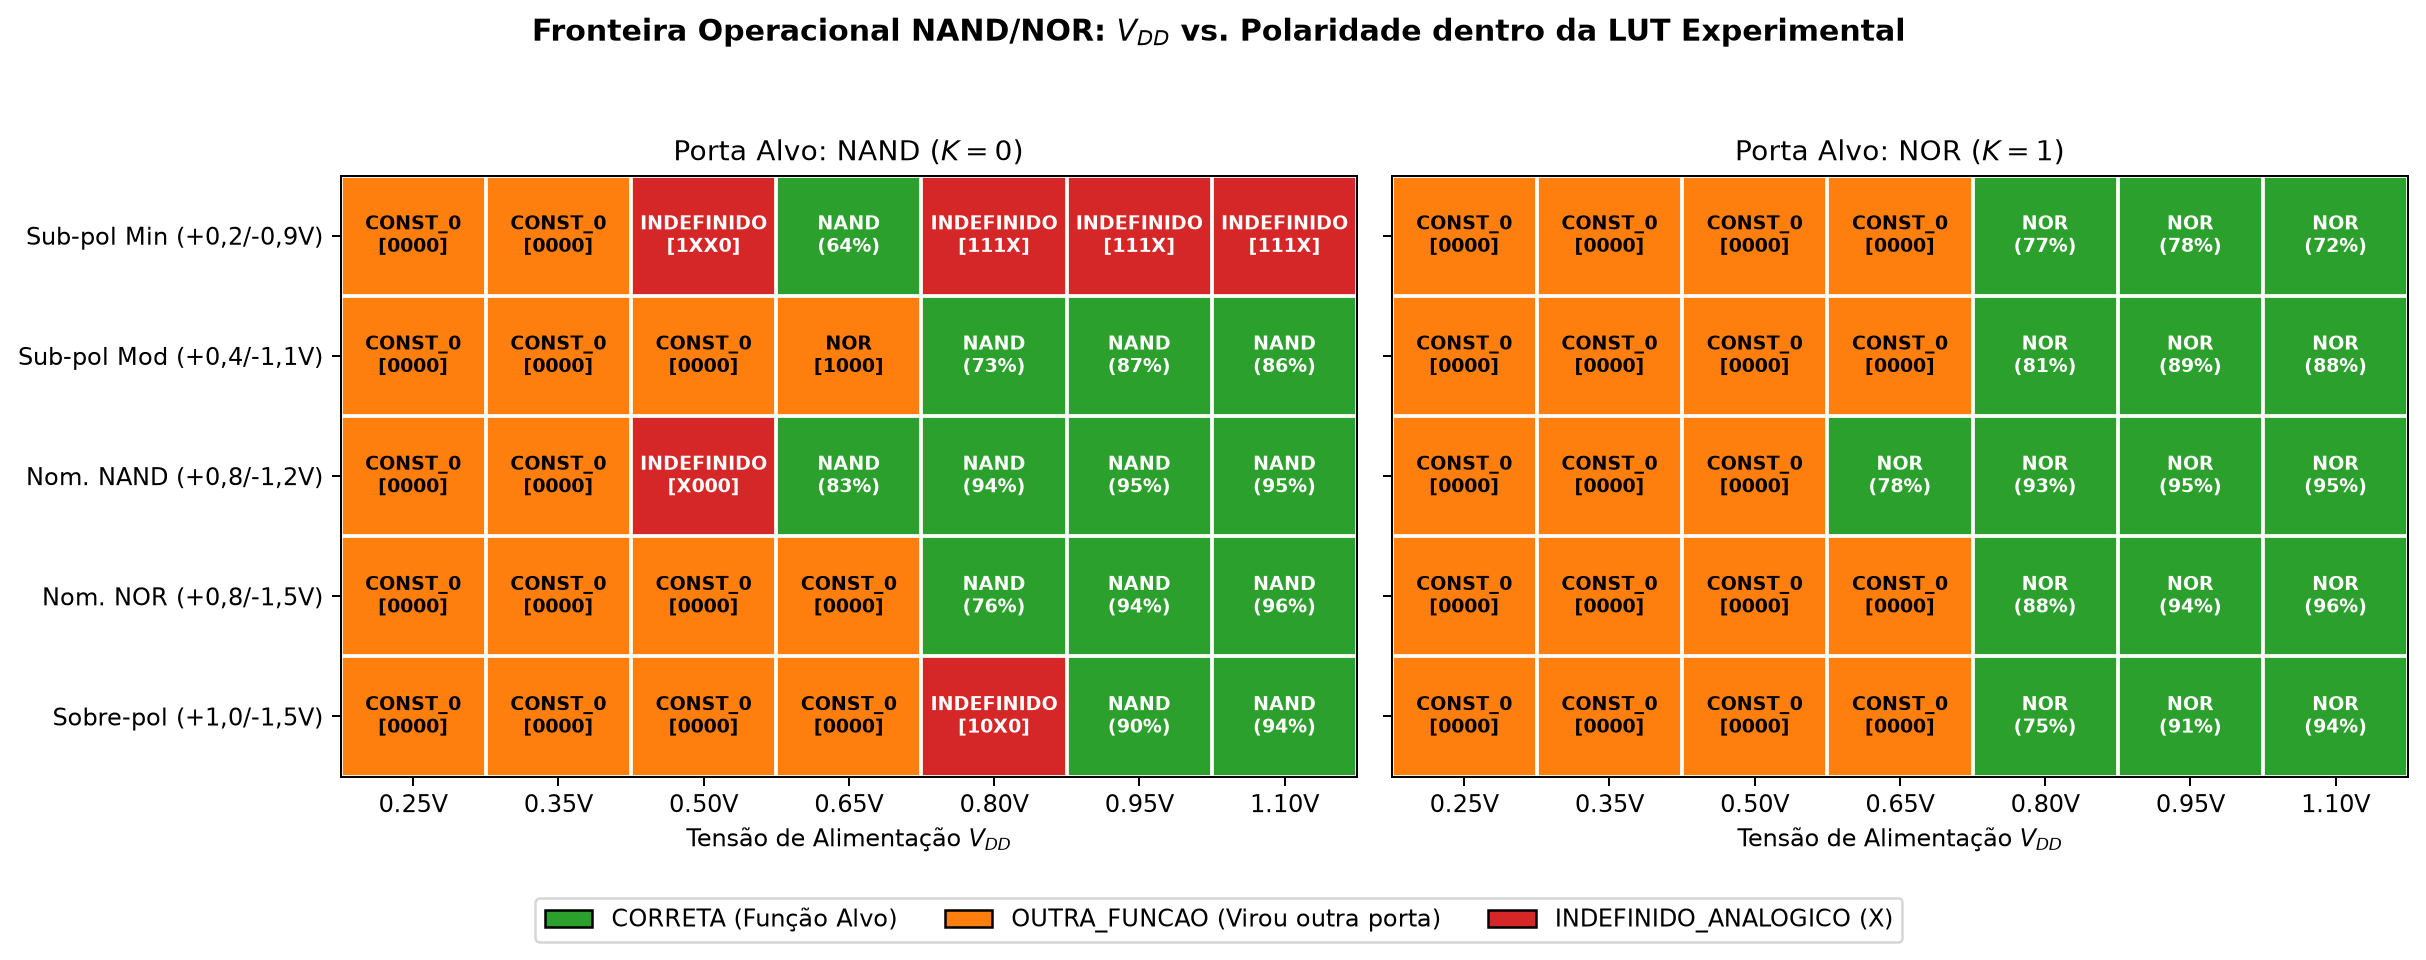
\includegraphics[width=0.92\textwidth]{m06_nand_nor_mapa_vdd_polaridade.png}
\caption{Operating phase map ($V_{DD} \times$ polarity) of the \texttt{NAND}/\texttt{NOR} gate, highlighting spontaneous \texttt{NAND} $\to$ \texttt{NOR} conversion at $V_{DD}=0.65\ \text{V}$ and \texttt{CONST\_0} collapse at under-voltage.}
\label{fig:m06_nn_vdd}
\end{figure}

\begin{figure}[htbp]
\centering
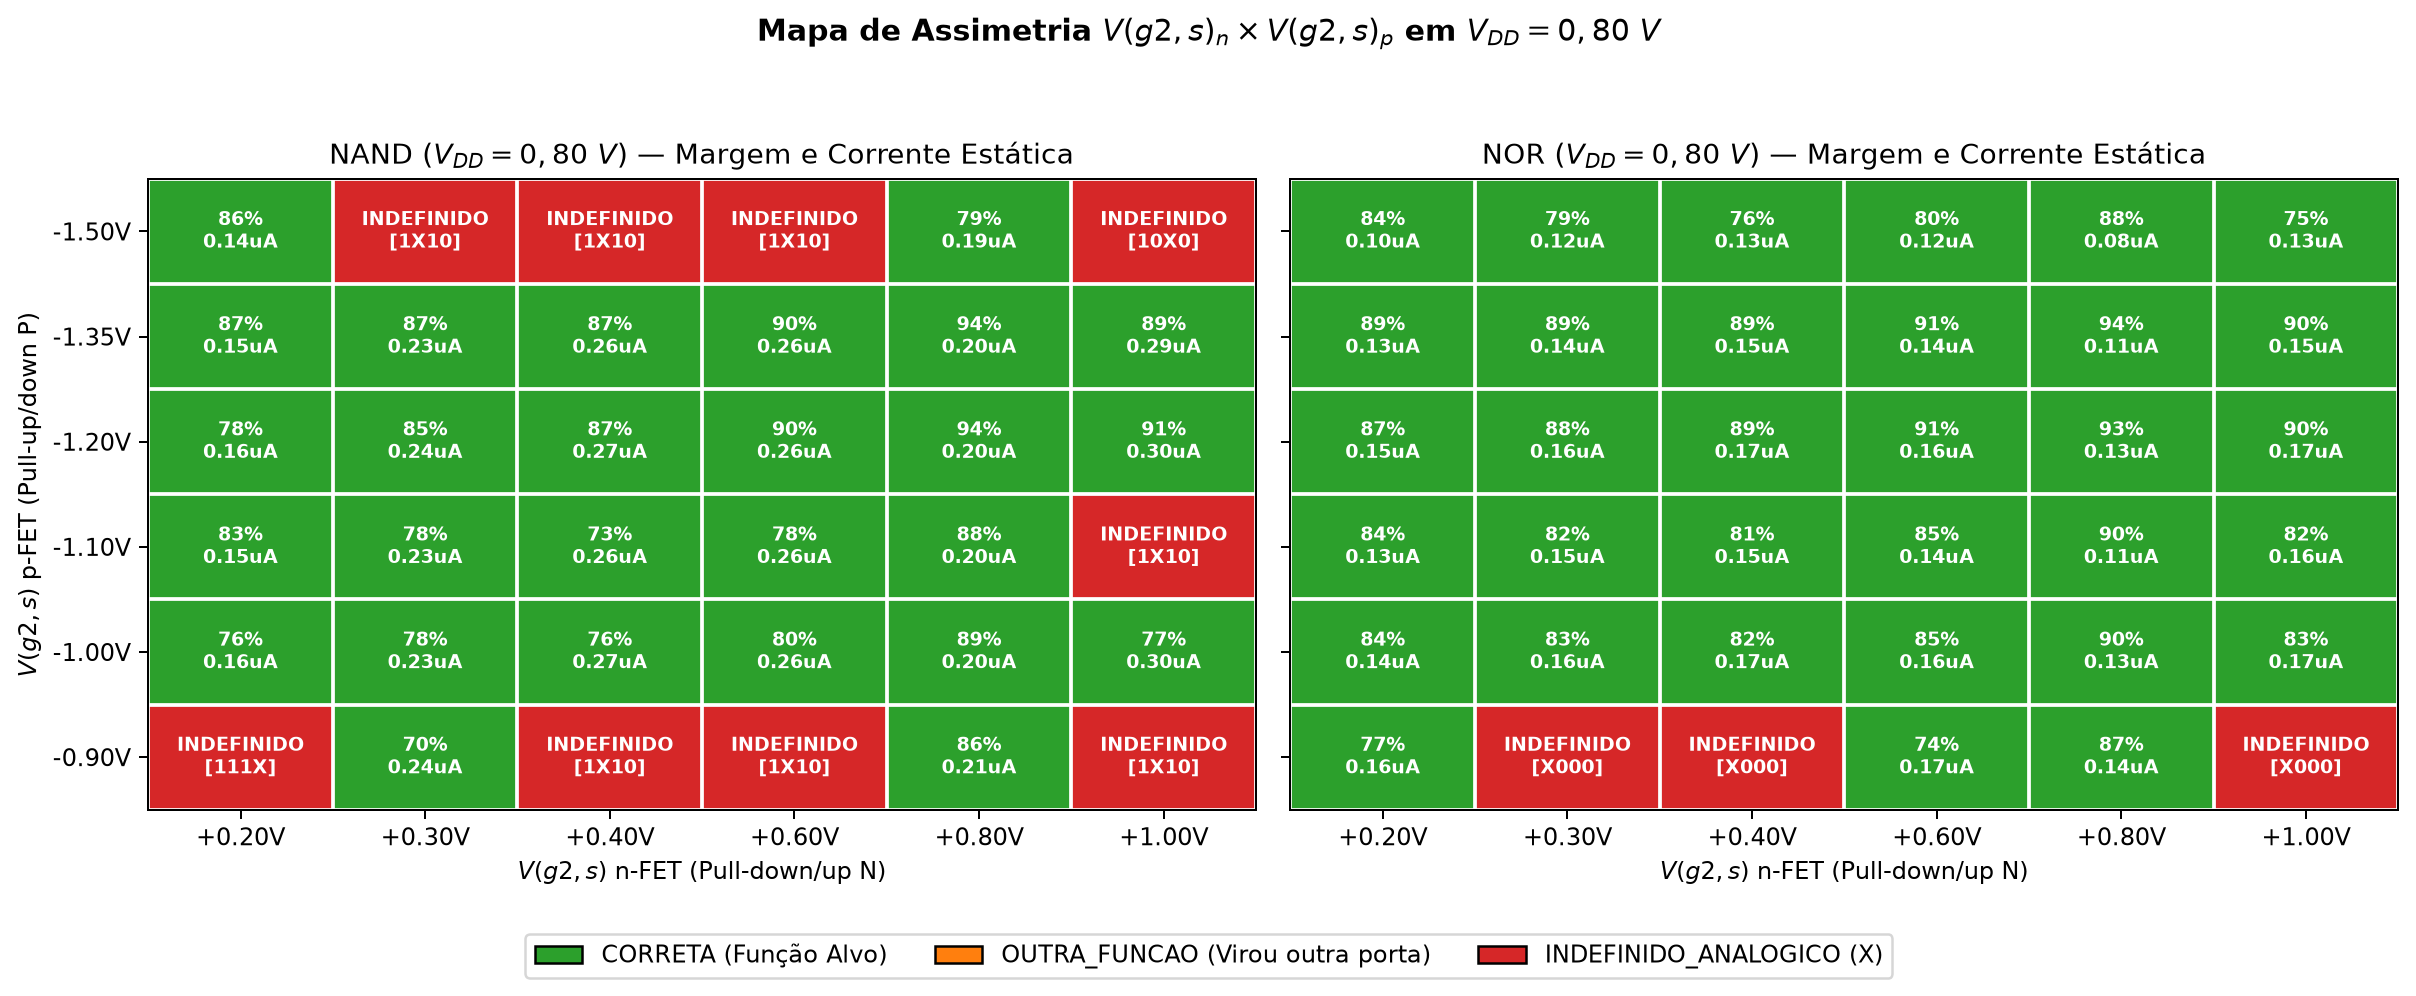
\includegraphics[width=0.92\textwidth]{m06_nand_nor_assimetria_vg2.png}
\caption{$V(g2,s)_n \times V(g2,s)_p$ asymmetry map at $V_{DD}=0.80\ \text{V}$ for \texttt{NAND} and \texttt{NOR}, exposing non-monotonic degradation at $V(g2,s)_p = -1.50\ \text{V}$.}
\label{fig:m06_nn_asym}
\end{figure}

\begin{figure}[htbp]
\centering
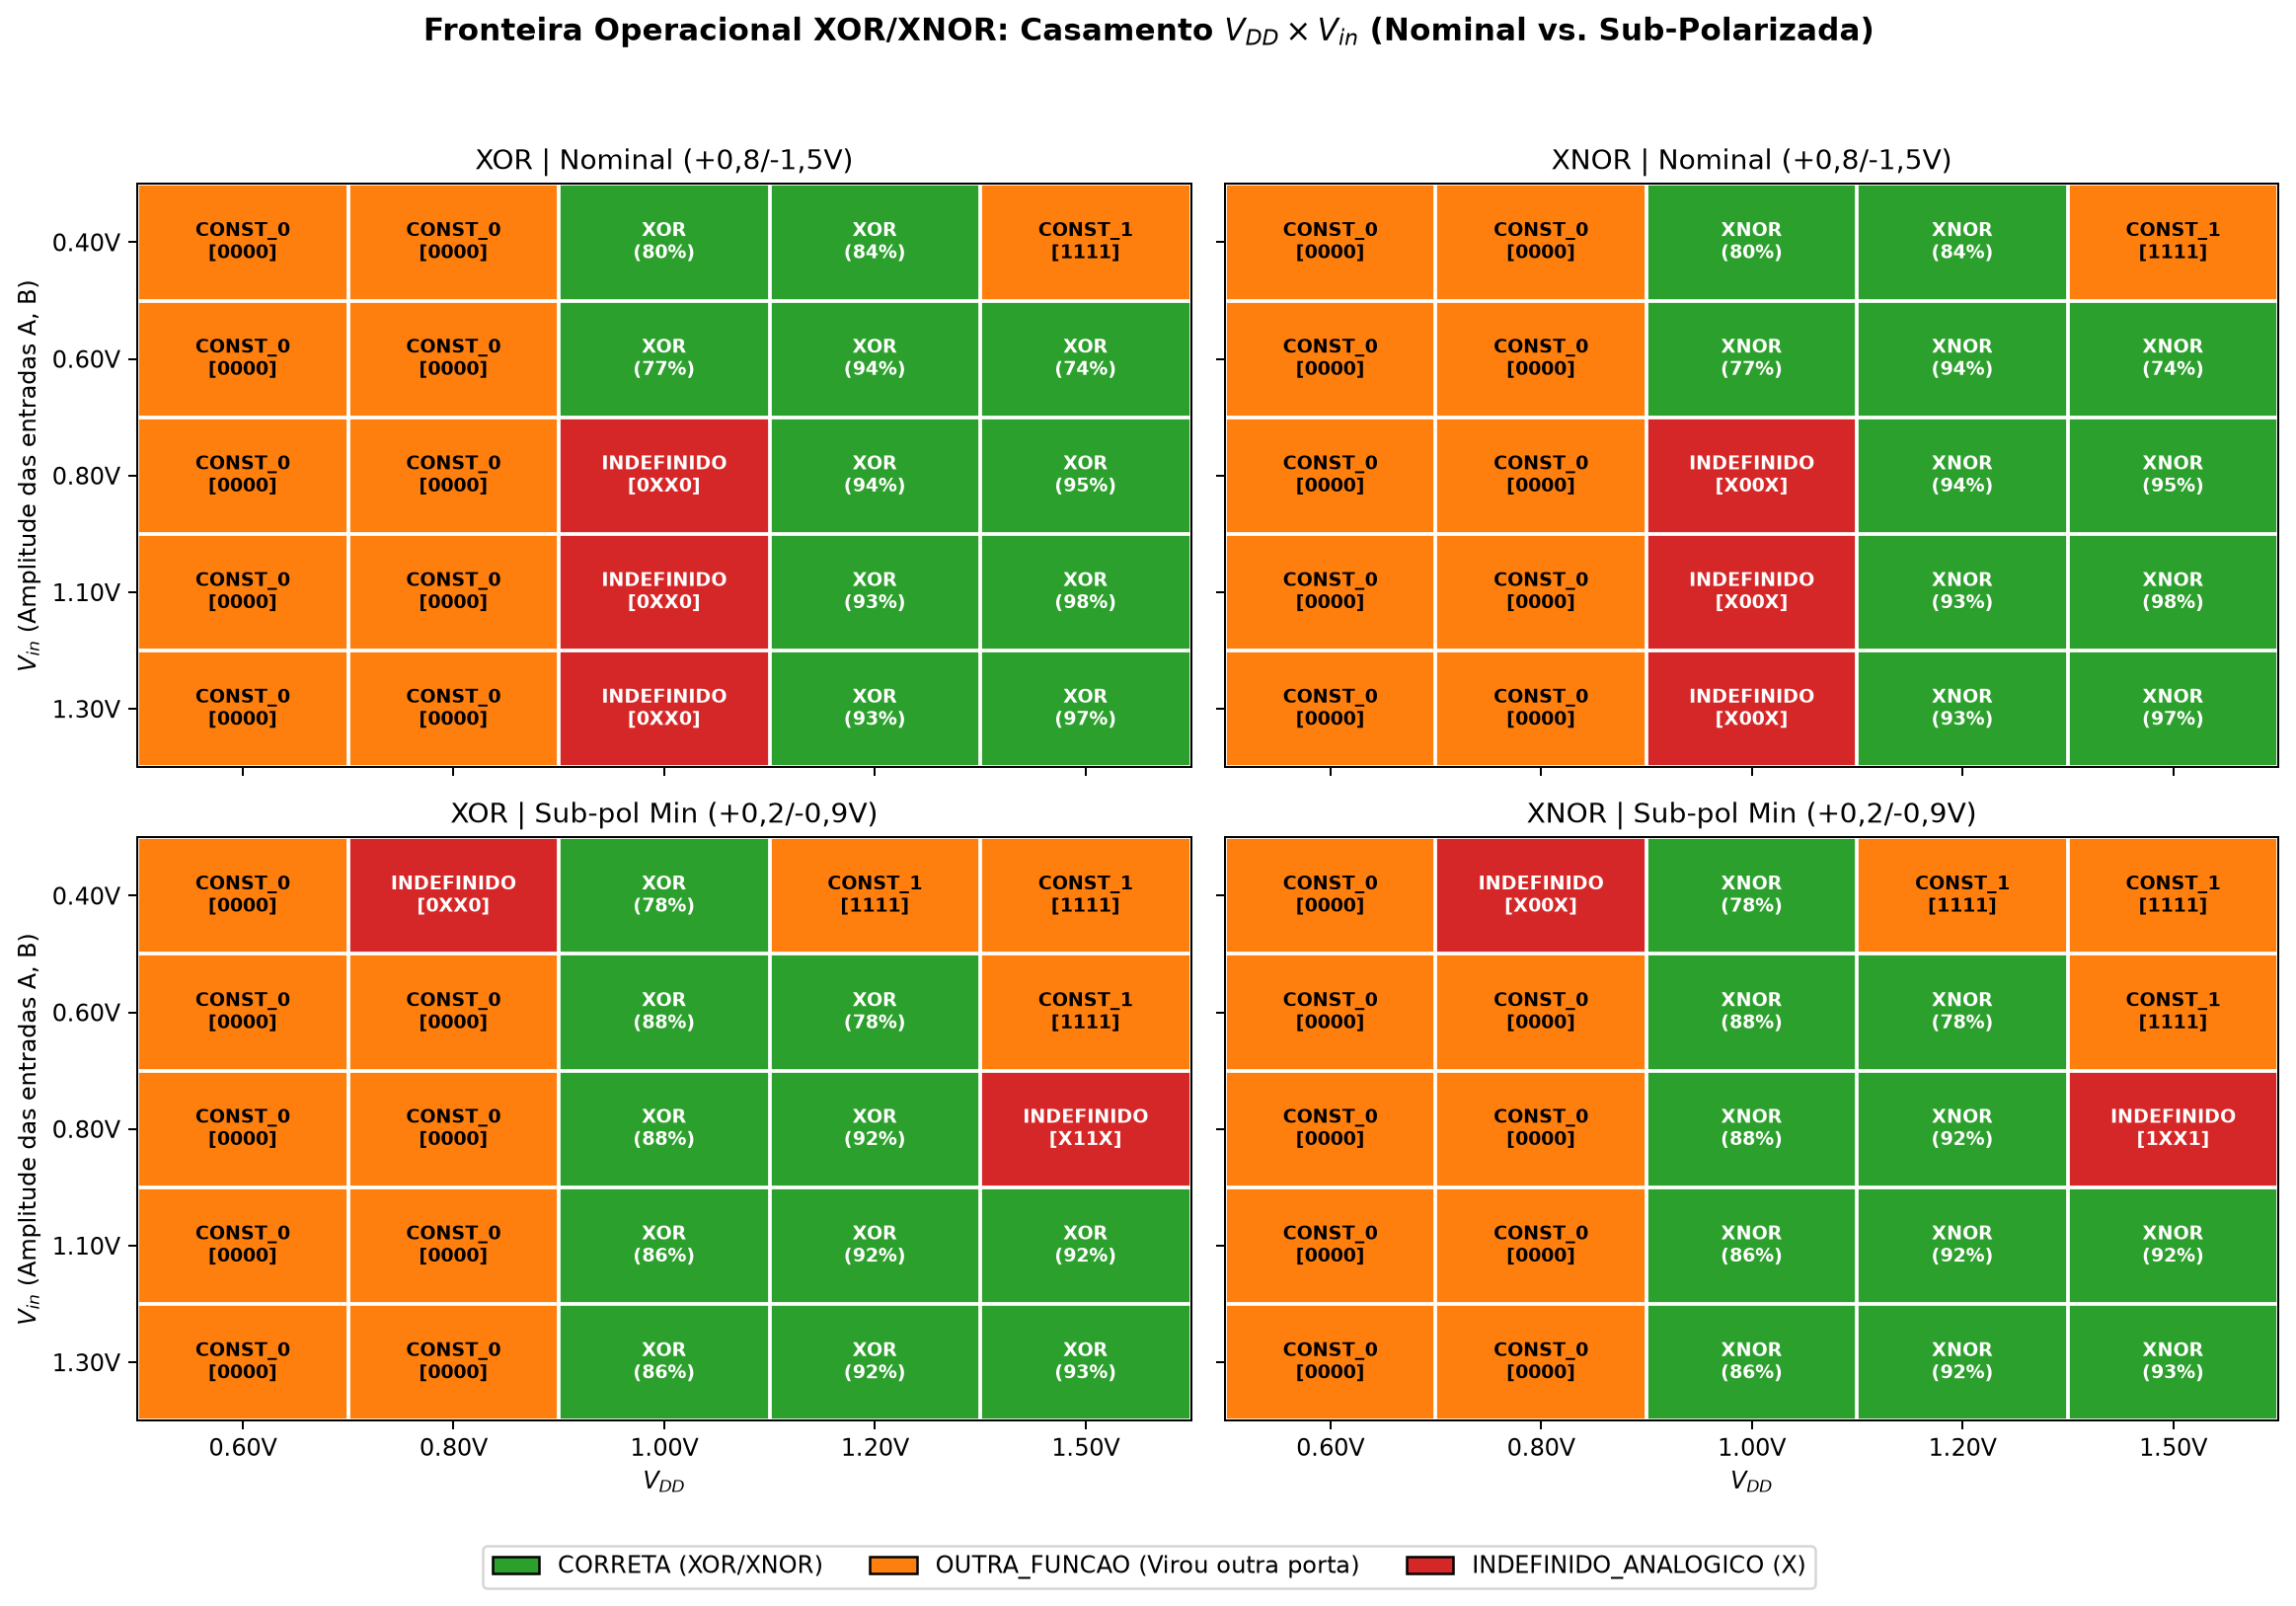
\includegraphics[width=0.92\textwidth]{m06_xor_xnor_mapa_vdd_vin.png}
\caption{$V_{DD} \times V_{\mathrm{in}}$ operating map of the \texttt{XOR}/\texttt{XNOR} gate under nominal bias, sub-polarization, and fixed gate voltage, illustrating \texttt{CONST\_0}, \texttt{CONST\_1}, and undefined regions.}
\label{fig:m06_xor_map}
\end{figure}

\subsection{DPA Asymmetry across Seven Polymorphic Tuples and Full Adder Benchmark}\label{sec:res_tuples}

In Module~\texttt{07}, all $72$ input-key combinations across the seven polymorphic tuples achieved $100.0\%$ functional correctness ($V_{1,\min} \ge 0.6792\ \text{V}$ at $0.8\ \text{V}$ and $\ge 1.3767\ \text{V}$ at $1.5\ \text{V}$; $V_{0,\max} \le 0.0128\ \text{V}$). Table~\ref{tab:tuples_dpa} compiles the hardware cost, DPA asymmetry, dynamic performance, and Monte Carlo robustness metrics.

\begin{table}[htbp]
\centering
\caption{Consolidated cost, DPA asymmetry, dynamic performance, and Monte Carlo robustness across seven polymorphic tuples ($C_{\mathrm{load}} = 0.3\ \text{fF}$).}
\label{tab:tuples_dpa}
\resizebox{\textwidth}{!}{%
\begin{tabular}{l c c c c c c c c c c c}
\toprule
\textbf{Tuple} & \textbf{Core/Tot.} & $\sum W$ ($\mu\text{m}$) & $V_{DD}$ (V) & $I_{\mathrm{peak}}$ M0/M1 ($\mu\text{A}$) & \textbf{Peak DPA} & \textbf{Avg.\ DPA} & $t_p$ (ps) & $P_{\mathrm{avg}}$ (nW) & $E_{\mathrm{sw}}$ (fJ) & \textbf{PDP} (aJ) & \textbf{MC} ($N=250$) \\
\midrule
\texttt{(NAND, NOR)}   & 4T / 4T   & $6.0$  & $0.8$ & $0.5643$ / $0.2138$ & $163.91\%$ & $44.62\%$ & $554.28$ & $40.17$  & $0.5022$ & $22.27$ & $100.00\%$ \\
\texttt{(XOR, XNOR)}   & 4T / 8T   & $4.0$  & $1.5$ & $1.6914$ / $1.6914$ & $0.00\%$   & $30.57\%$ & $151.84$ & $102.47$ & $1.2808$ & $15.56$ & $100.00\%$ \\
\texttt{(AND, OR)}     & 6T / 6T   & $9.0$  & $0.8$ & $1.7345$ / $1.8394$ & $6.05\%$   & $30.87\%$ & $454.27$ & $48.04$  & $0.6005$ & $21.82$ & $100.00\%$ \\
\texttt{(NAND, XNOR)}  & 6T / 10T  & $8.0$  & $1.5$ & $1.7050$ / $1.3387$ & $27.36\%$  & $73.87\%$ & $163.46$ & $94.14$  & $1.1768$ & $15.39$ & $100.00\%$ \\
\texttt{(NOR, XOR)}    & 6T / 10T  & $8.0$  & $1.5$ & $1.7129$ / $1.6932$ & $1.16\%$   & $29.60\%$ & $144.87$ & $121.49$ & $1.5186$ & $17.60$ & $100.00\%$ \\
\texttt{(AOI21, OAI21)}& 6T / 6T   & $12.0$ & $0.8$ & $0.6810$ / $0.4299$ & $58.44\%$  & $19.22\%$ & $555.72$ & $59.97$  & $0.4498$ & $33.33$ & $99.55\%$  \\
\texttt{(MAJ3, XOR3)}  & 10T / 18T & $18.0$ & $1.5$ & $1.4360$ / $1.4355$ & $0.04\%$   & $47.08\%$ & $180.71$ & $212.44$ & $1.9119$ & $38.39$ & $100.00\%$ \\
\bottomrule
\end{tabular}}
\end{table}

Under the standardized \texttt{ngspice-47} testbench, the current traces (Figure~\ref{fig:m07_signatures}) and Pareto frontier (Figure~\ref{fig:m07_pareto}) reveal distinct design trade-offs:
\begin{itemize}
    \item \texttt{(NAND, NOR)} achieves minimal physical cost ($4\text{T}$, $40.17\ \text{nW}$) at the expense of severe peak DPA exposure ($163.91\%$) and high delay ($554.28\ \text{ps}$) caused by asymmetry between parallel ($W=1.0$) and series ($W=2.0$) stacks.
    \item \texttt{(XOR, XNOR)} completely eliminates peak asymmetry ($0.00\%$, $1.6914\ \mu\text{A}$ in both modes) with a low PDP of $15.56\ \text{aJ}$.
    \item In \texttt{(AND, OR)}, appending the \texttt{BP\_INV08} output inverter ($+2\text{T}$) isolates the load from the polymorphic core and reduces overall supply peak asymmetry to $6.05\%$, although asymmetry across $1 \to 0$ falling edges remains substantial ($116.90\%$).
    \item Among mixed-locking cells, \texttt{(NOR, XOR)} offers an outstanding trade-off ($1.16\%$ peak DPA asymmetry and the lowest delay in the suite at $144.87\ \text{ps}$), whereas \texttt{(NAND, XNOR)} exhibits high average asymmetry ($73.87\%$) due to the \texttt{'1'}-probability imbalance between \texttt{NAND} ($75\%$) and \texttt{XNOR} ($50\%$).
    \item For 3-input cells, \texttt{(AOI21, OAI21)} delivers the lowest time-averaged asymmetry ($19.22\%$) and lowest switching energy ($0.4498\ \text{fJ}$) in $6\text{T}$, with a slight Monte Carlo drop ($99.55\%$, Figure~\ref{fig:m07_mc}) under stacked \texttt{OAI21} conduction; conversely, \texttt{(MAJ3, XOR3)} extends quad-symmetric balance to three inputs with $0.04\%$ peak DPA asymmetry and $100.0\%$ Monte Carlo yield.
\end{itemize}

\begin{figure}[htbp]
\centering
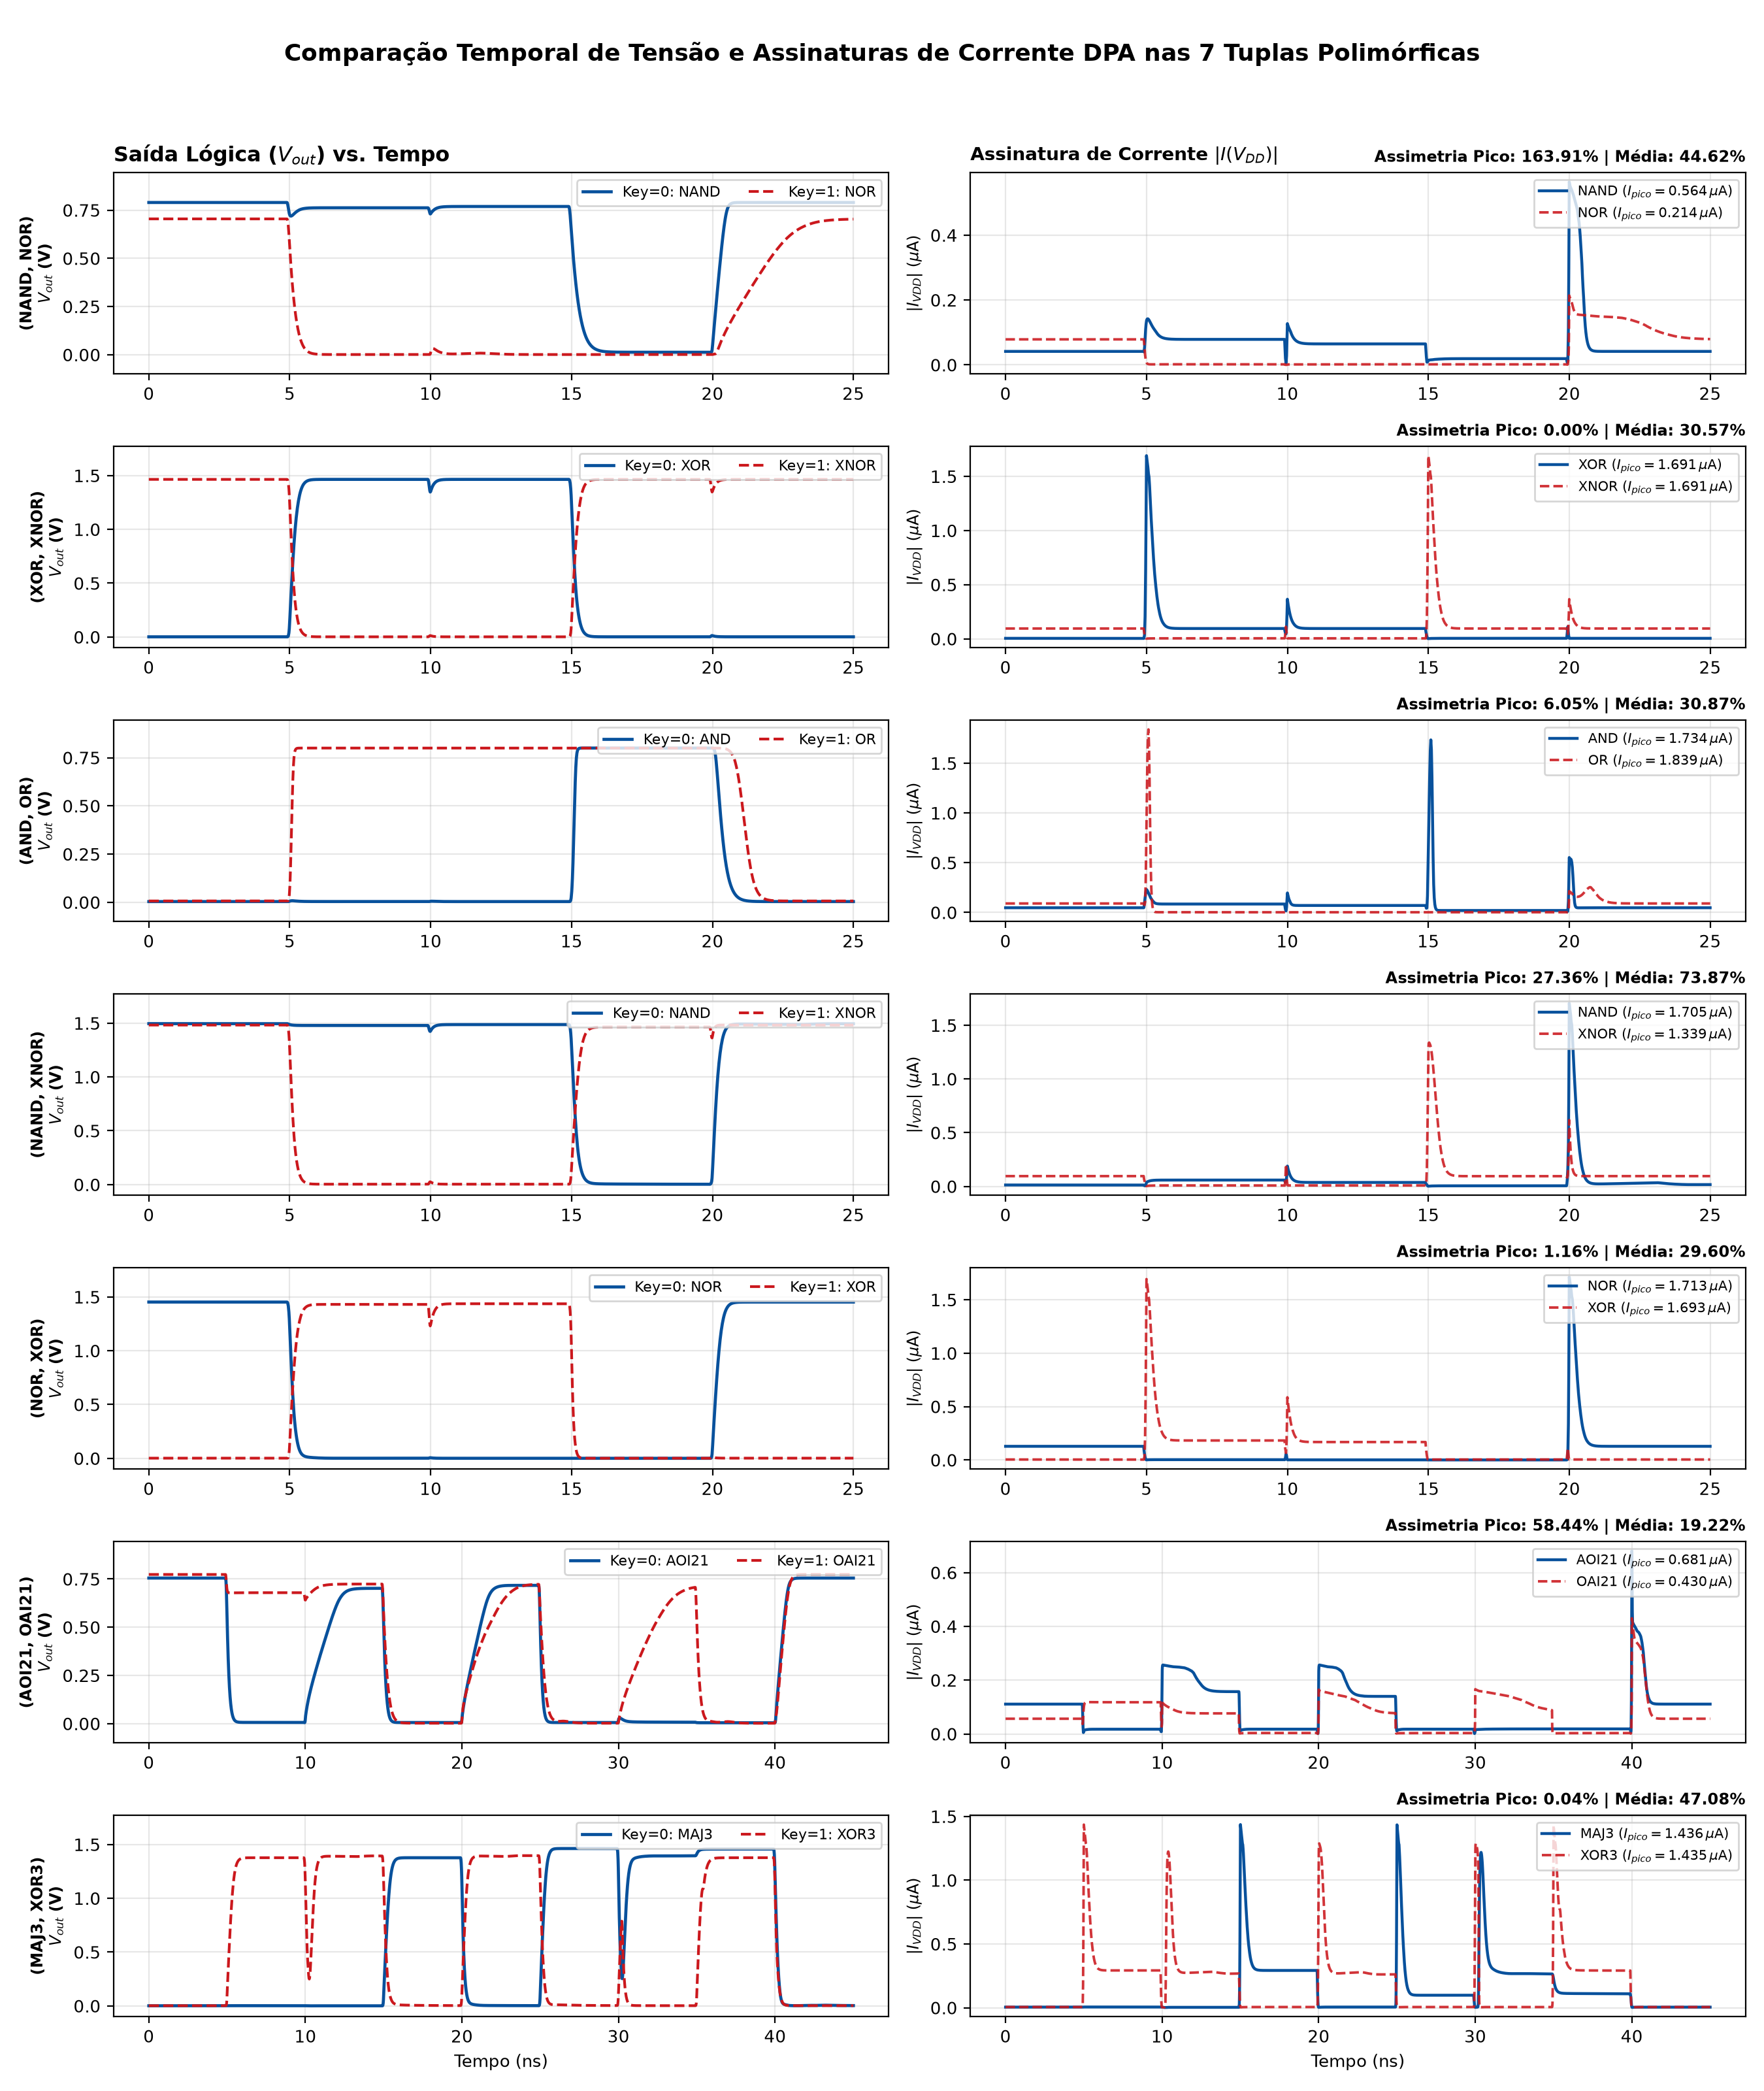
\includegraphics[width=0.90\textwidth,height=0.76\textheight,keepaspectratio]{m07_assinaturas_corrente_tuplas.png}
\caption{Supply current signatures $|I(V_{DD})|$ comparing $\text{Key}=0$ and $\text{Key}=1$ across the seven polymorphic tuples under standardized capacitive load ($C_{\mathrm{load}} = 0.3\ \text{fF}$).}
\label{fig:m07_signatures}
\end{figure}

\begin{figure}[htbp]
\centering
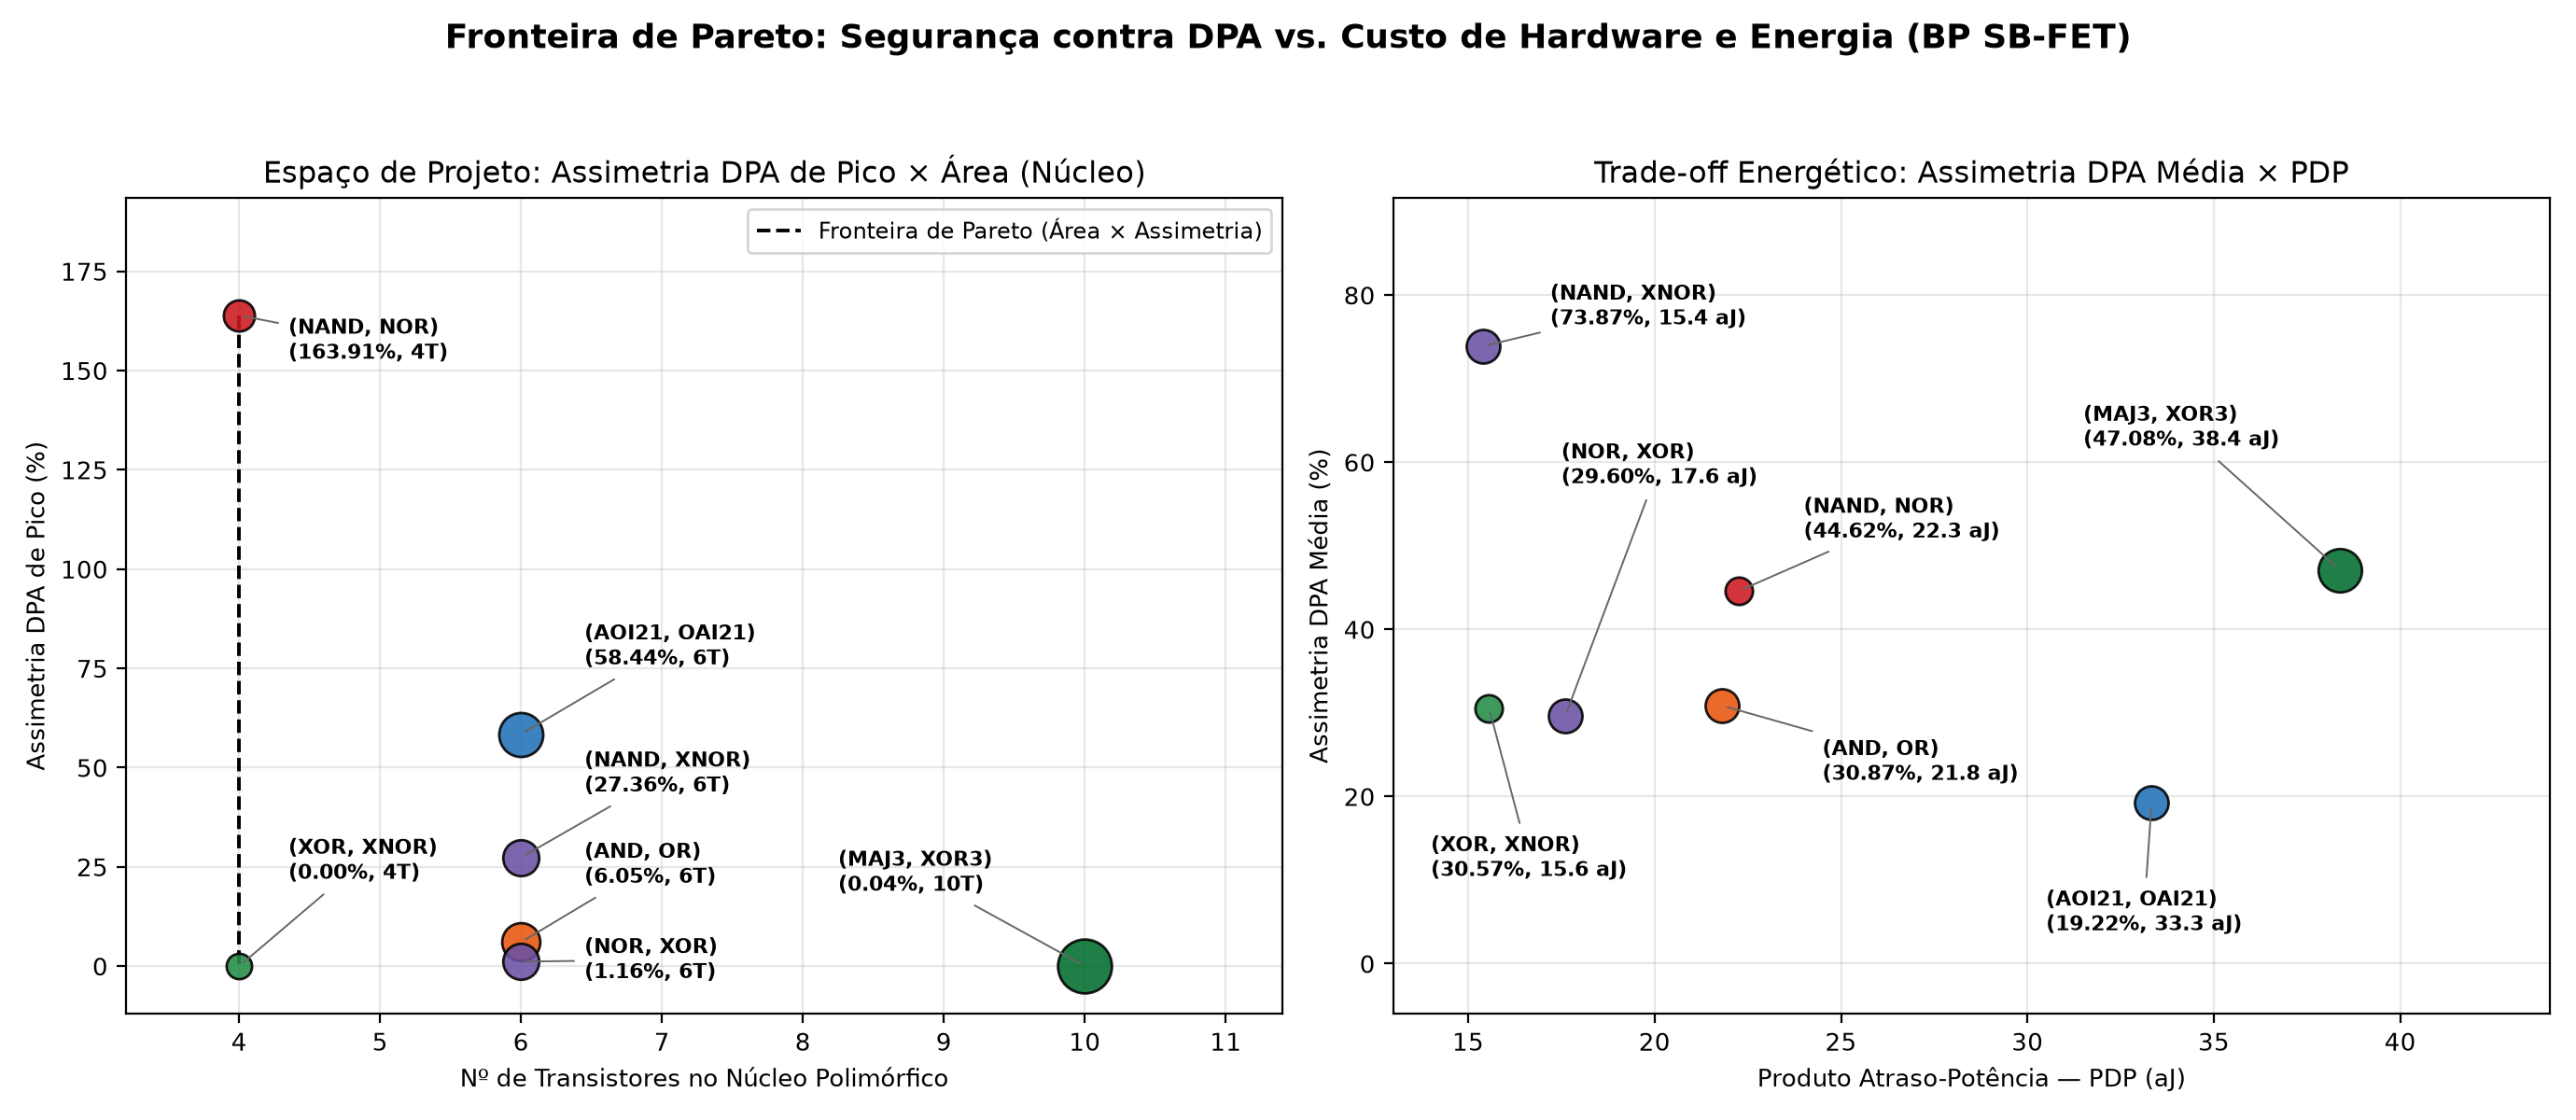
\includegraphics[width=0.92\textwidth]{m07_pareto_assimetria_vs_custo.png}
\caption{Pareto frontier relating peak DPA asymmetry, transistor count, and power-delay product ($\mathrm{PDP}$) across the seven evaluated tuples.}
\label{fig:m07_pareto}
\end{figure}

\begin{figure}[htbp]
\centering
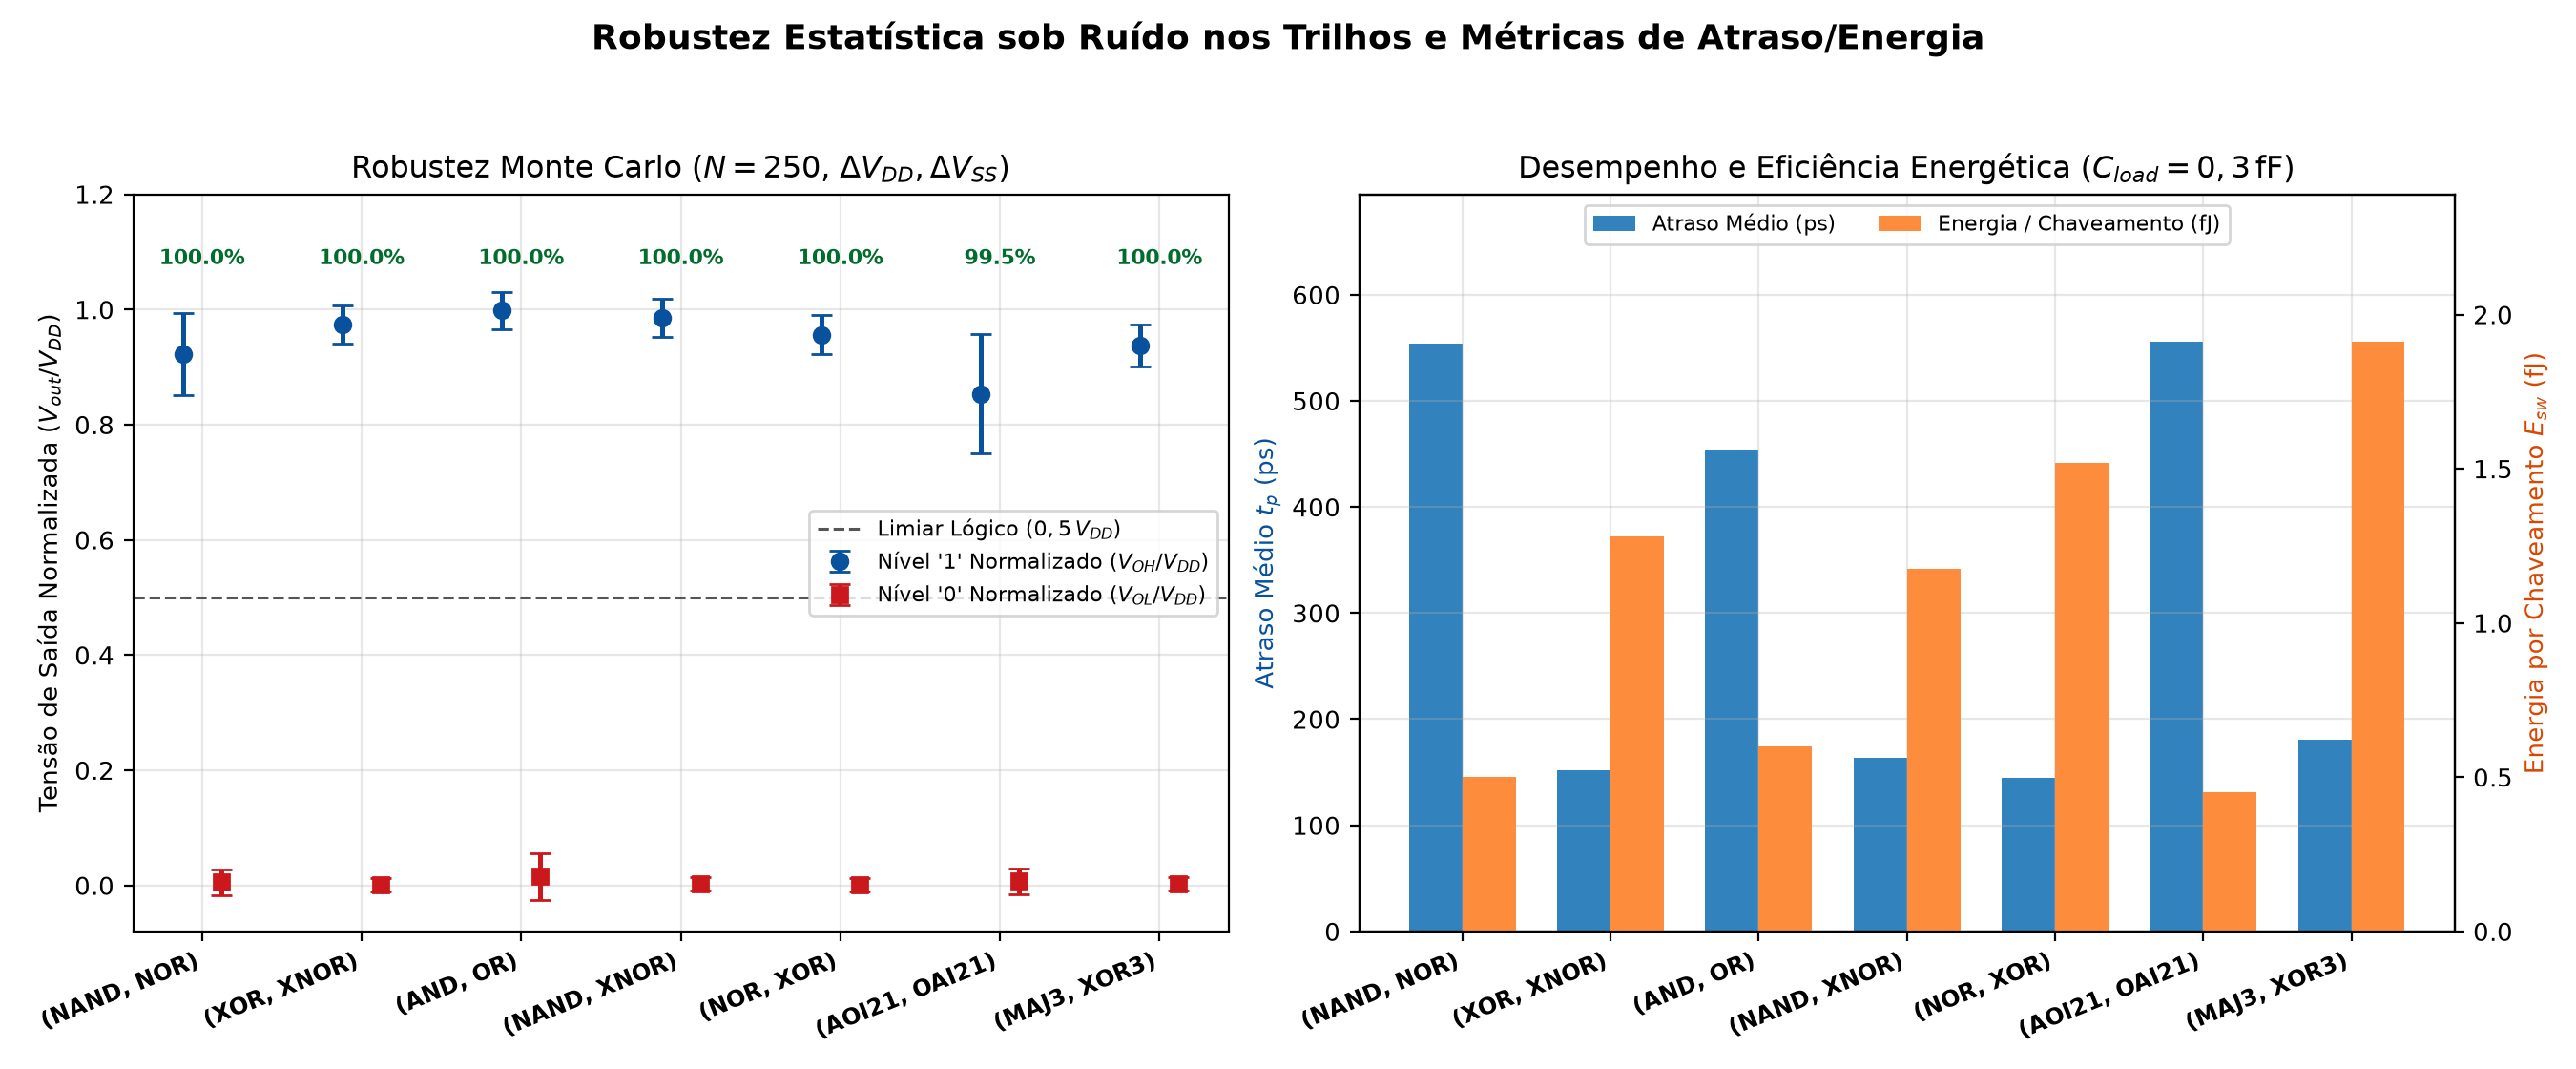
\includegraphics[width=0.92\textwidth]{m07_robustez_montecarlo_tuplas.png}
\caption{Monte Carlo yield ($N=250$) under realistic supply-rail noise and delay/energy distributions across the seven tuples.}
\label{fig:m07_mc}
\end{figure}

In the system-level 1-bit Full Adder benchmark (Table~\ref{tab:fa_profiles} and Figure~\ref{fig:m07_fa}), all three architectures achieved $100.0\%$ accuracy under $K=00$. \textbf{Profile 2} (using three \texttt{NAND}/\texttt{NOR} gates for carry) increases core count to 28T, multiplies critical delay by $3.58\times$ over the Baseline ($177.72 \to 636.68\ \text{ps}$), raises critical PDP by $3.54\times$ ($131.86 \to 466.44\ \text{aJ}$), and leaks a $113.83\%$ peak DPA signature on the carry stage. By contrast, \textbf{Profile 3} replaces the \texttt{NAND}/\texttt{NOR} tree with a single 10T \texttt{(MAJ3, XOR3)} gate, cutting core count to 26T, raising wrong-key ($K=11$) Hamming Distance from $68.75\%$ to $87.50\%$, and slashing peak DPA asymmetry in the polymorphic carry stage from $113.83\%$ down to just \textbf{$0.04\%$}. With a critical delay of $196.98\ \text{ps}$ ($+10.8\%$ over Baseline) and PDP of $155.19\ \text{aJ}$ ($+17.7\%$ over Baseline and \textbf{$3.01\times$ lower than Profile 2}), Profile 3 simultaneously excels in security, area, and energy efficiency.

\begin{table}[htbp]
\centering
\caption{System-level 1-bit Full Adder benchmark across three architectural profiles in \texttt{ngspice-47} ($C_{\mathrm{load}} = 0.3\ \text{fF}$).}
\label{tab:fa_profiles}
\resizebox{\textwidth}{!}{%
\begin{tabular}{l c c c c c c c c c}
\toprule
\textbf{Architectural Profile} & \textbf{Core} & $\sum W$ & \textbf{K00 Acc.} & \textbf{HD (K11)} & $t_{\mathrm{crit}}$ (ps) & $P_{\mathrm{avg}}$ (nW) & \textbf{PDP} (aJ) & \textbf{Carry Peak DPA} & \textbf{Carry Avg.\ DPA} \\
\midrule
1. Baseline (Common, unlocked) & 20T & $24.0$ & $100.0\%$ & $0.0\%$   & $177.72$ & $741.97$ & $131.86$ & N/A & N/A \\
2. Cost/Perf.\ (\texttt{NAND}/\texttt{NOR}) & 28T & $38.0$ & $100.0\%$ & $68.75\%$ & $636.68$ & $732.60$ & $466.44$ & $113.83\%$ & $62.44\%$ \\
3. Low Asymmetry (\texttt{MAJ3}/\texttt{XOR3}) & 26T & $38.0$ & $100.0\%$ & $87.50\%$ & $196.98$ & $787.87$ & $155.19$ & $0.04\%$   & $47.47\%$ \\
\bottomrule
\end{tabular}}
\end{table}

\begin{figure}[htbp]
\centering
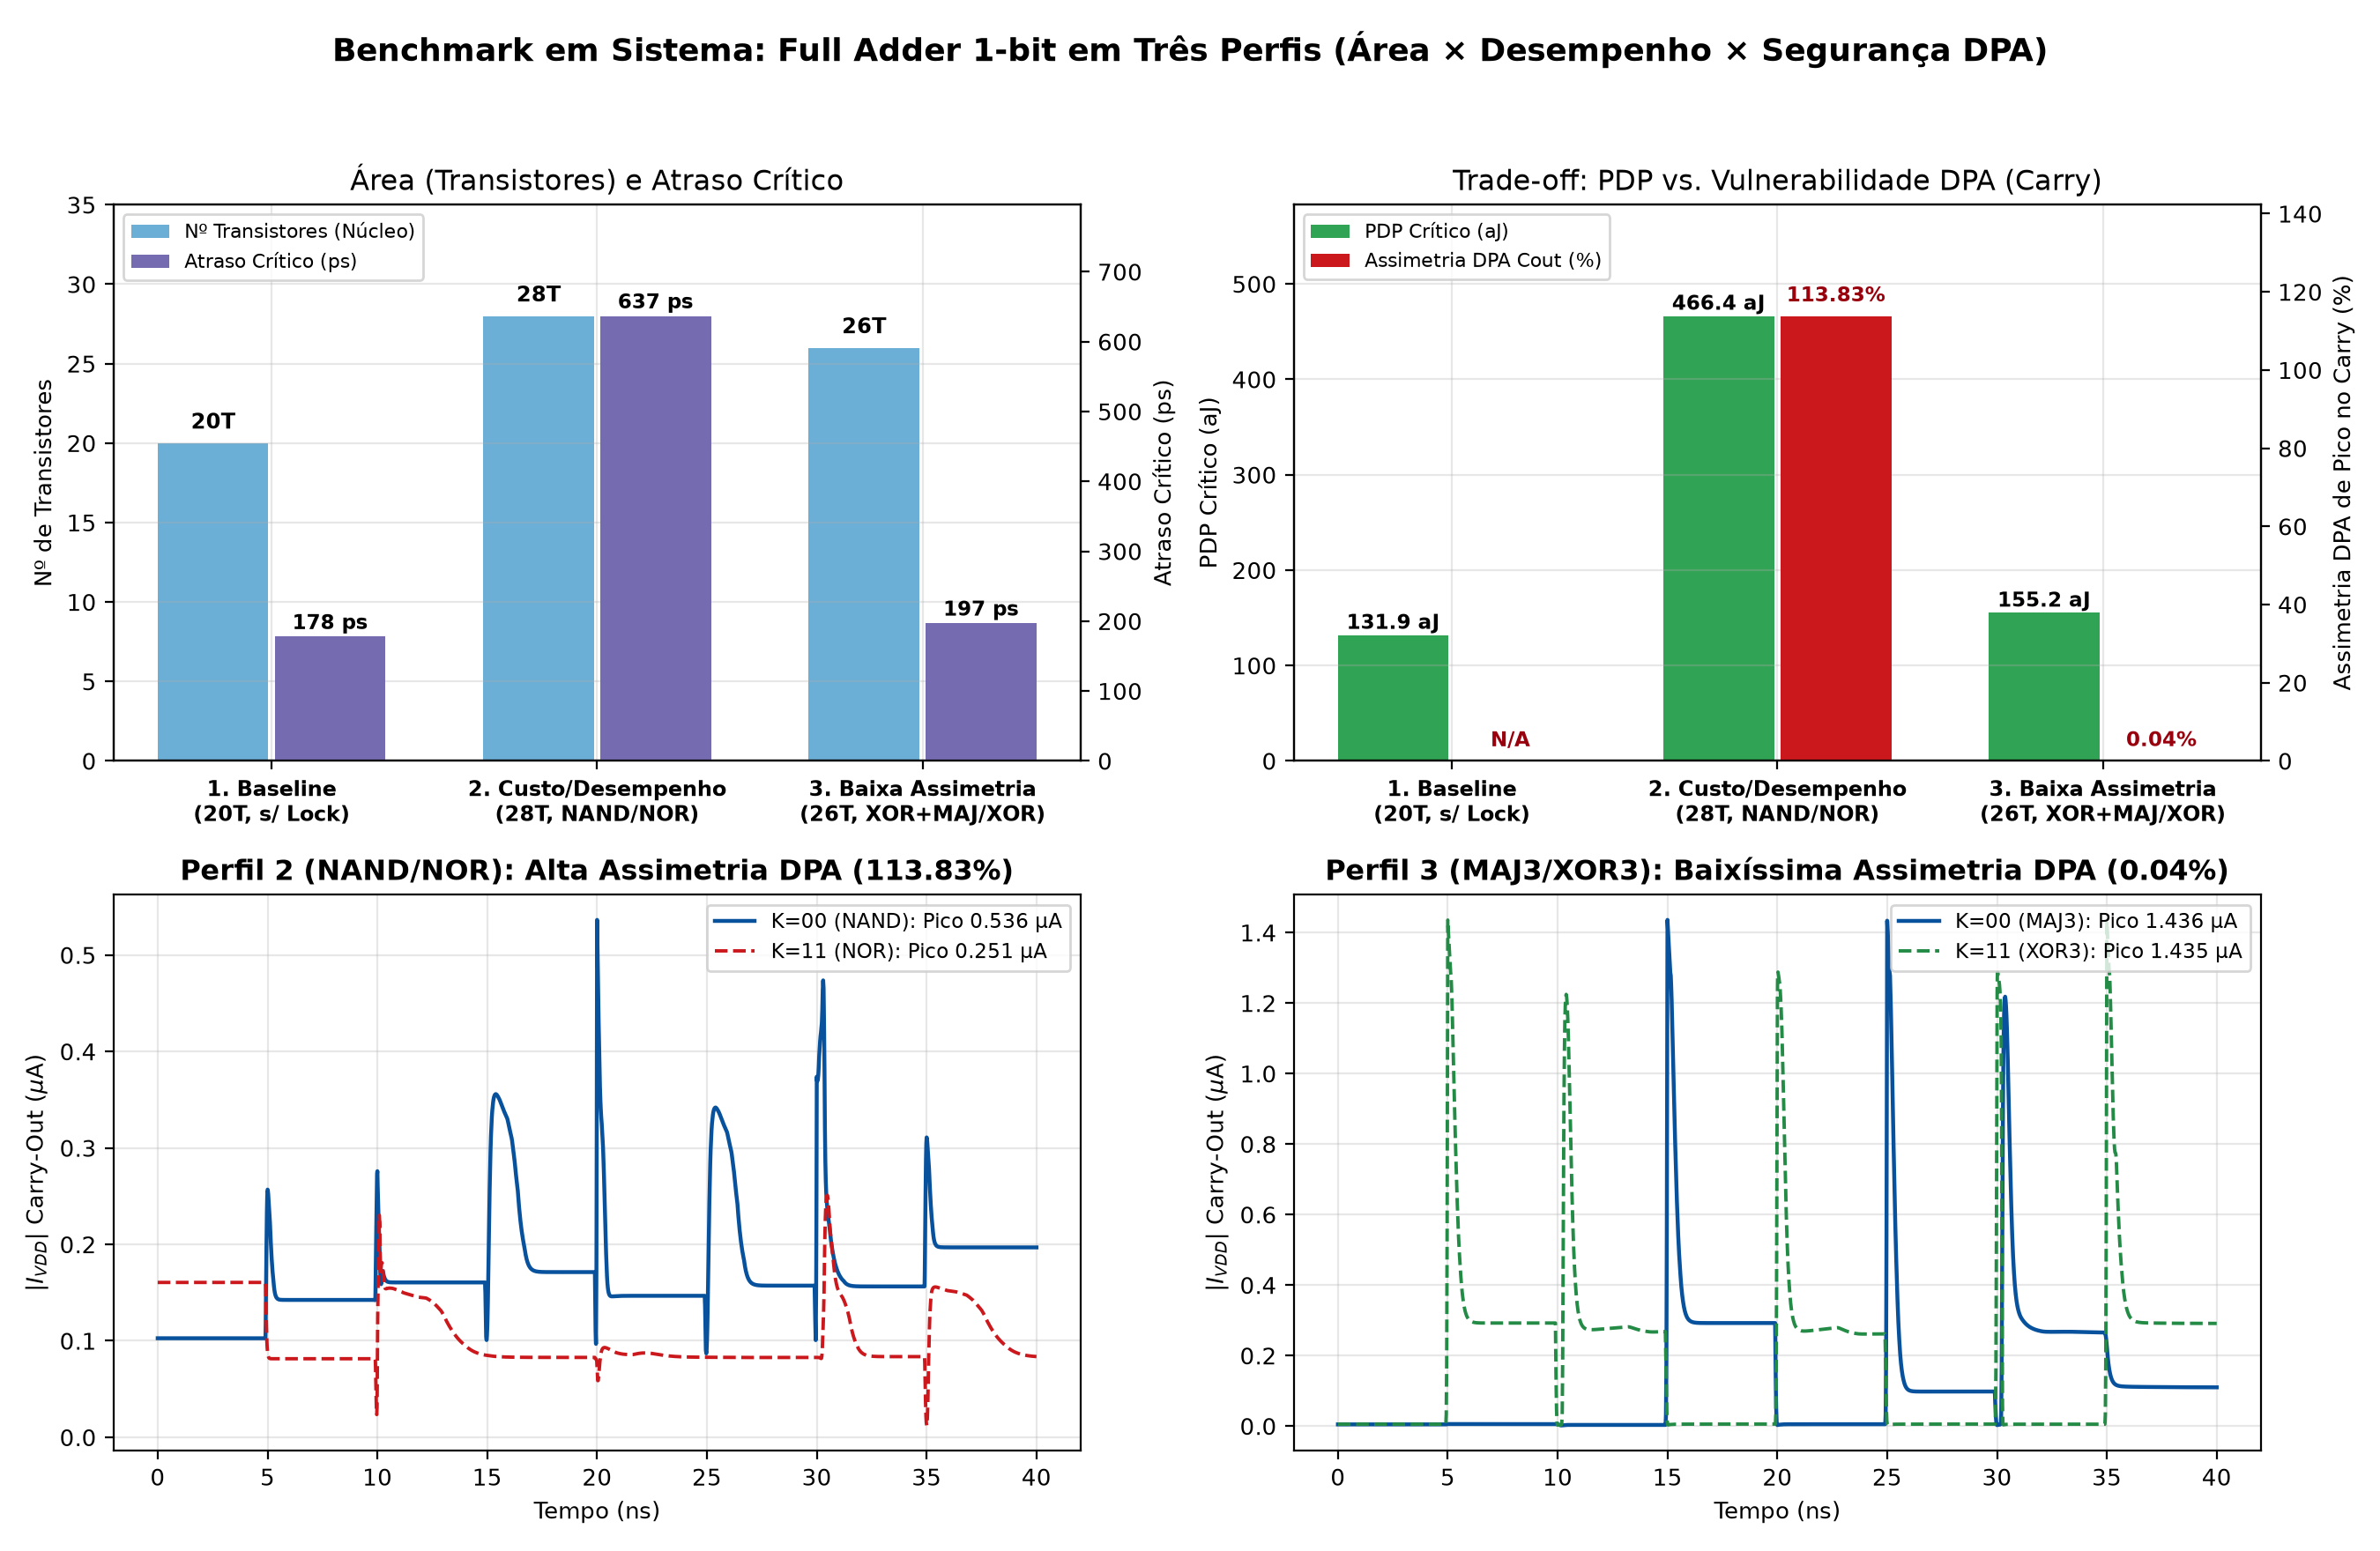
\includegraphics[width=0.92\textwidth]{m07_benchmark_full_adder_perfis.png}
\caption{Comparison of the three 1-bit Full Adder architectural profiles across transistor count, critical delay, PDP, wrong-key obfuscation (HD), and carry DPA asymmetry.}
\label{fig:m07_fa}
\end{figure}

\subsection{End-to-End Validation of the Interactive Visual Simulator (\textit{BP-FET Studio})}\label{sec:res_web}

The automated test suite \texttt{simulador\_web/test\_simulator.py} fully validated graph compilation, batch \texttt{ngspice-47} execution, and the REST backend of \textit{BP-FET Studio}:
\begin{enumerate}
    \item \textbf{Seven polymorphic tuples and \texttt{INV} at high level:} every truth-table row and \textit{X-Ray} transistor mapping passed with $100\%$ accuracy, reproducing the Module~\texttt{07} peak DPA asymmetry metrics (\texttt{NAND\_NOR}: $163.91\%$; \texttt{XOR\_XNOR}: $0.00\%$; \texttt{AND\_OR}: $6.05\%$; \texttt{NAND\_XNOR}: $27.36\%$; \texttt{NOR\_XOR}: $1.16\%$; \texttt{AOI21\_OAI21}: $58.44\%$; \texttt{MAJ3\_XOR3}: $0.04\%$; \texttt{INV}: $0.00\%$) in execution times from $234\ \text{ms}$ (\texttt{INV}) to $7.04\ \text{s}$ (\texttt{MAJ3\_XOR3}).
    \item \textbf{Eight catalog templates:} all high- and low-level circuits passed ($0.65\ \text{s}$ to $14.31\ \text{s}$), verifying both Full Adder Profiles 2 and 3 at $K=0$, physical polarity flipping (\textit{p-FET} $\leftrightarrow$ \textit{n-FET}) in the 4T \texttt{NAND}/\texttt{NOR} cell, and retention ($\Delta V > 0.7\ \text{V}$ at $12\ \text{ns}$, \texttt{XPU1} as \textit{p-FET}) followed by collapse ($\Delta V < 0.25\ \text{V}$ at $28\ \text{ns}$, \texttt{XPU1} as \textit{n-FET}) in the 6T SRAM.
    \item \textbf{Mixed multi-domain cascade and HTTP API:} an arbitrary mixed-voltage chain $0.8\ \text{V} \to 1.5\ \text{V} \to 0.8\ \text{V}$ (\texttt{NAND\_\allowbreak NOR} $\to$ \texttt{XOR\_\allowbreak XNOR} $\to$ \texttt{AND\_\allowbreak OR}) with automatic level conditioning compiled and passed in $5.87\ \text{s}$ ($100\%$ exact for $\text{Key}=0$ and $\text{Key}=1$), and all HTTP/JSON endpoints (\texttt{/}, \texttt{/api/\allowbreak tuples}, \texttt{/api/\allowbreak templates}, \texttt{/api/\allowbreak simulate}) returned HTTP $200$.
\end{enumerate}

\section{Conclusion}\label{sec:conclusion}

This work established and validated a complete, open-source computational ecosystem in \texttt{ngspice-47} and Python for behavioral modeling, physical characterization, hardware security evaluation, and visual prototyping of digital circuits based on two-dimensional BP SB-FET devices. Translating the 4D experimental surfaces with bilateral source referencing and gate-specific saturation curves (\texttt{bp\_ari\_ngspice.lib} \texttt{v2}) eliminated the proprietary dependency on Synopsys HSPICE/Verilog-A with mean error below $0.0621\%$ against the source tables, achieved $R^2 \ge 0.99977$ across \texttt{N\_transfer}, \texttt{P\_transfer}, and \texttt{P\_output}, and reduced \textit{p-FET} output RMSE by $196\times$ by explicitly capturing the measured $V_{g2} = -1.5\ \text{V}$ regime.

At the circuit and security levels, electrostatic $V_{fb}$ compensation preserved differential voltage gain above unity ($|A_v| = 2.71$) and $89.75\%$ output swing down to $V_{DD} = 0.2\ \text{V}$ in the complementary inverter. The 4-transistor \texttt{NAND}/\texttt{NOR} and \texttt{XOR}/\texttt{XNOR} polymorphic primitives attained $100\%$ dynamic truth-table accuracy with $0\%$ transistor overhead and $100.0\%$ yield across $250$ Monte Carlo supply-rail noise samples. In the 6T SRAM cell, Mechanism B was validated under fixed power rails: tuning $V_{g2,\mathrm{PU}} = -0.2\ \text{V}$ achieved $\Delta V_{\mathrm{Key0}} = 0.9747\ \text{V}$ and $\mathrm{SNM}_{\mathrm{Hold}} = 167.12\ \text{mV}$ under the authorized key, whereas $\text{Key}=1$ collapsed retention to $\mathrm{SNM} = 0.00\ \text{mV}$ ($\Delta V_{\mathrm{Key1}} = 0.0762\ \text{V}$), with \textit{Read Disturb} mitigated via \textit{Wordline Underdrive Read-Assist} ($\mathrm{SNM}_{\mathrm{Read,Assist}} = 66.23\ \text{mV}$ at $\mathrm{WL}=0.30\ \text{V}$).

Probing operating boundaries outside nominal biases within the measured LUT domain confirmed three distinct physical regimes: alongside robust nominal windows and stuck-at degeneration (\texttt{CONST\_0} at under-voltage and \texttt{CONST\_1} under asymmetric overdrive in \texttt{XOR}/\texttt{XNOR}), a spontaneous key-less \texttt{NAND} $\to$ \texttt{NOR} conversion was demonstrated at $V_{DD}=0.65\ \text{V}$ ($+0.4/-1.1\ \text{V}$), demarcating voltage margins relevant to fault-injection resilience. Across the seven-tuple DPA Pareto frontier, \texttt{(XOR, XNOR)} ($0.00\%$), \texttt{(MAJ3, XOR3)} ($0.04\%$), and \texttt{(NOR, XOR)} ($1.16\%$) stood out against the $163.91\%$ peak exposure of \texttt{(NAND, NOR)}. At the system level on a 1-bit Full Adder, replacing the 3-gate \texttt{NAND}/\texttt{NOR} carry tree with a single symmetric \texttt{(MAJ3, XOR3)} cell reduced carry-stage peak DPA asymmetry from $113.83\%$ to $0.04\%$, saved 2 transistors, increased wrong-key corruption to $87.50\%$, and lowered critical PDP by $3.01\times$, capabilities also exposed interactively through \textit{BP-FET Studio}.

With respect to methodological limitations inherited from the experimental lookup tables, the library \texttt{bp\_\allowbreak ari\_\allowbreak ngspice.lib} preserves the quasi-static formulation of \texttt{bp\_\allowbreak ari.va} without intrinsic parasitic capacitances ($C_{gs}$, $C_{gd}$, $C_{g2s}$), temperature dependence, or process variability ($\sigma_{V_{fb}}, \sigma_W$); consequently, propagation delays, switching energies, and absolute PDP values depend directly on the explicit testbench capacitances ($0.05\text{--}1.0\ \text{fF}$), while the unmeasured interval $V(g2,s) \in (-0.90,\allowbreak\ +0.20)\ \text{V}$ remained excluded to avoid ungrounded extrapolation. Future work includes embedding parasitic capacitive networks and statistical process parameters into the \texttt{ARI} subcircuit, scaling the 6T SRAM into $2 \times 2$ and $4 \times 4$ arrays with \textit{Write Margin} and sneak-path analysis, and extending the low-DPA polymorphic adder to multi-bit arithmetic datapaths and cryptographic primitives evaluated against SAT and correlation power analysis (CPA) attacks.


\bibliographystyle{ieeetr}
\bibliography{references}

\end{document}
